\documentclass[twoside]{book}

% Packages required by doxygen
\usepackage{calc}
\usepackage{doxygen}
\usepackage{graphicx}
\usepackage[utf8]{inputenc}
\usepackage{makeidx}
\usepackage{multicol}
\usepackage{multirow}
\usepackage{textcomp}
\usepackage[table]{xcolor}

% Font selection
\usepackage[T1]{fontenc}
\usepackage{mathptmx}
\usepackage[scaled=.90]{helvet}
\usepackage{courier}
\usepackage{amssymb}
\usepackage{sectsty}
\renewcommand{\familydefault}{\sfdefault}
\allsectionsfont{%
  \fontseries{bc}\selectfont%
  \color{darkgray}%
}
\renewcommand{\DoxyLabelFont}{%
  \fontseries{bc}\selectfont%
  \color{darkgray}%
}

% Page & text layout
\usepackage{geometry}
\geometry{%
  a4paper,%
  top=2.5cm,%
  bottom=2.5cm,%
  left=2.5cm,%
  right=2.5cm%
}
\tolerance=750
\hfuzz=15pt
\hbadness=750
\setlength{\emergencystretch}{15pt}
\setlength{\parindent}{0cm}
\setlength{\parskip}{0.2cm}
\makeatletter
\renewcommand{\paragraph}{%
  \@startsection{paragraph}{4}{0ex}{-1.0ex}{1.0ex}{%
    \normalfont\normalsize\bfseries\SS@parafont%
  }%
}
\renewcommand{\subparagraph}{%
  \@startsection{subparagraph}{5}{0ex}{-1.0ex}{1.0ex}{%
    \normalfont\normalsize\bfseries\SS@subparafont%
  }%
}
\makeatother

% Headers & footers
\usepackage{fancyhdr}
\pagestyle{fancyplain}
\fancyhead[LE]{\fancyplain{}{\bfseries\thepage}}
\fancyhead[CE]{\fancyplain{}{}}
\fancyhead[RE]{\fancyplain{}{\bfseries\leftmark}}
\fancyhead[LO]{\fancyplain{}{\bfseries\rightmark}}
\fancyhead[CO]{\fancyplain{}{}}
\fancyhead[RO]{\fancyplain{}{\bfseries\thepage}}
\fancyfoot[LE]{\fancyplain{}{}}
\fancyfoot[CE]{\fancyplain{}{}}
\fancyfoot[RE]{\fancyplain{}{\bfseries\scriptsize Generated on Sun Feb 16 2014 21\-:23\-:09 for S\-D\-L2\-Me by Doxygen }}
\fancyfoot[LO]{\fancyplain{}{\bfseries\scriptsize Generated on Sun Feb 16 2014 21\-:23\-:09 for S\-D\-L2\-Me by Doxygen }}
\fancyfoot[CO]{\fancyplain{}{}}
\fancyfoot[RO]{\fancyplain{}{}}
\renewcommand{\footrulewidth}{0.4pt}
\renewcommand{\chaptermark}[1]{%
  \markboth{#1}{}%
}
\renewcommand{\sectionmark}[1]{%
  \markright{\thesection\ #1}%
}

% Indices & bibliography
\usepackage{natbib}
\usepackage[titles]{tocloft}
\setcounter{tocdepth}{3}
\setcounter{secnumdepth}{5}
\makeindex

% Hyperlinks (required, but should be loaded last)
\usepackage{ifpdf}
\ifpdf
  \usepackage[pdftex,pagebackref=true]{hyperref}
\else
  \usepackage[ps2pdf,pagebackref=true]{hyperref}
\fi
\hypersetup{%
  colorlinks=true,%
  linkcolor=blue,%
  citecolor=blue,%
  unicode%
}

% Custom commands
\newcommand{\clearemptydoublepage}{%
  \newpage{\pagestyle{empty}\cleardoublepage}%
}


%===== C O N T E N T S =====

\begin{document}

% Titlepage & ToC
\hypersetup{pageanchor=false}
\pagenumbering{roman}
\begin{titlepage}
\vspace*{7cm}
\begin{center}%
{\Large S\-D\-L2\-Me }\\
\vspace*{1cm}
{\large Generated by Doxygen 1.8.5}\\
\vspace*{0.5cm}
{\small Sun Feb 16 2014 21:23:09}\\
\end{center}
\end{titlepage}
\clearemptydoublepage
\tableofcontents
\clearemptydoublepage
\pagenumbering{arabic}
\hypersetup{pageanchor=true}

%--- Begin generated contents ---
\chapter{S\-D\-L2\-Me Tutorial}
\label{index}\hypertarget{index}{}\hypertarget{index_intro_sec}{}\section{Introduction}\label{index_intro_sec}
S\-D\-L2\-Me, or S2\-M for short, is a library that uses S\-D\-L2 in order to bring a more familiar game development environment, implementing concepts such as Sprites, Cameras, Rooms, etc. It is inspired in the way Game Maker software (by Yo\-Yo\-Games) handles game programming.\hypertarget{index_actual_use_sec}{}\section{Actual use example}\label{index_actual_use_sec}
This is an example of how to initialise the libraries and draw a simple \hyperlink{class_sprite}{Sprite} on the screen\-: 
\begin{DoxyCode}
\textcolor{preprocessor}{#include "\hyperlink{_s2_m_8h}{S2M.h}"}

\textcolor{comment}{// Create an Options instance by checking the config file specified.}
\textcolor{comment}{// This will load all configurations into memory.}
\hyperlink{class_options}{Options} gOptions = \hyperlink{class_options}{Options}(\textcolor{stringliteral}{"config.cfg"});

\textcolor{comment}{// Create the Graphics instance based on the game screen size specified and the Options instance.}
\hyperlink{class_graphics}{Graphics} gGraphics = \hyperlink{class_graphics}{Graphics}(320,240,\textcolor{stringliteral}{"S2M Test"},&\hyperlink{class_options}{Options});

\textcolor{comment}{// Create a Room and make it current.}
\hyperlink{class_room}{Room} gRoom = \hyperlink{class_room}{Room}(); \textcolor{comment}{// Default black Room}
gGraphics.setCurrentRoom(gRoom);

\textcolor{comment}{// Create a first and only Sprite.}
\hyperlink{class_sprite}{Sprite} *test = gGraphics.createSprite(\textcolor{stringliteral}{"test.bmp"},16,16,0);
test->x = 0;
test->y = 0;

\textcolor{comment}{// Game Loop}
\textcolor{keywordflow}{while} (\textcolor{keyword}{true}) \{

    \textcolor{comment}{// Update the graphics}
    gGraphics.\hyperlink{class_graphics_a5a5297a160c22f73300dcf72ac0be7c2}{update}()
\}
\end{DoxyCode}
 \hypertarget{index_ideal_use_sec}{}\section{I\-D\-E\-A\-L use example}\label{index_ideal_use_sec}
This is an example of how to initialise the libraries and draw a simple \hyperlink{class_sprite}{Sprite} on the screen, following the desired patterns and main goals to accomplish of these libraries. 
\begin{DoxyCode}
\textcolor{preprocessor}{#include "\hyperlink{_s2_m_8h}{S2M.h}"}

\textcolor{comment}{// Create an Options instance by checking the config file specified.}
\textcolor{comment}{// This will load all configurations into memory.}
\hyperlink{class_options}{Options} gOptions = \hyperlink{class_options}{Options}(\textcolor{stringliteral}{"config.cfg"});

\textcolor{comment}{// Create the Graphics instance based on the game screen size specified and the Options instance.}
\hyperlink{class_graphics}{Graphics} gGraphics = \hyperlink{class_graphics}{Graphics}(320,240,\textcolor{stringliteral}{"S2M Test"},&\hyperlink{class_options}{Options});

\textcolor{comment}{// Create a Room and make it current.}
\hyperlink{class_room}{Room} gRoom = \hyperlink{class_room}{Room}(); \textcolor{comment}{// Default black Room}
S2M\_MakeCurrentRoom(gRoom);

\textcolor{comment}{// Create a first and only Sprite.}
\hyperlink{class_sprite}{Sprite} *testSprite = gGraphics.createSprite(\textcolor{stringliteral}{"test.bmp"},16,16,0); \textcolor{comment}{// After this it still won't show in
       the screen.}

\textcolor{comment}{// Create an object bound to that Sprite.}
\hyperlink{class_object}{Object} *testObject = gRoom.\hyperlink{class_room_a0c09098560d165c23287969c77c702cc}{createObject}(testSprite);

\textcolor{comment}{// Game Loop}
\textcolor{keywordflow}{while} (\textcolor{keyword}{true}) \{

    \textcolor{comment}{// Update the room}
    \hyperlink{room_8cpp_a7e17b634091c660ba4b52f5a0940d7e4}{S2M\_UpdateRoom}();   \textcolor{comment}{// Will call the current Room's update method}
                        \textcolor{comment}{// The current Room's update method will call each object's update method.}
                        \textcolor{comment}{// Each object's update method will update its associated sprite's position.}
                        \textcolor{comment}{// The Graphics instance handles the Sprites update method, so no need for those
       calls here...}

    \textcolor{comment}{// Update the graphics}
    gGraphics.\hyperlink{class_graphics_a5a5297a160c22f73300dcf72ac0be7c2}{update}()
\}
\end{DoxyCode}
\hypertarget{index_step1}{}\subsection{Step 1\-: Opening the box}\label{index_step1}
etc... 
\chapter{Functions}
\label{_functions}
\hypertarget{_functions}{}
\input{_functions}
\chapter{Namespace Index}
\section{Namespace List}
Here is a list of all namespaces with brief descriptions\-:\begin{DoxyCompactList}
\item\contentsline{section}{\hyperlink{namespace_s2_m___room}{S2\-M\-\_\-\-Room} \\*Every \hyperlink{class_room}{Room} operation is included here }{\pageref{namespace_s2_m___room}}{}
\item\contentsline{section}{\hyperlink{namespace_s2_m___script}{S2\-M\-\_\-\-Script} \\*Scripting operations are included here }{\pageref{namespace_s2_m___script}}{}
\end{DoxyCompactList}

\chapter{Hierarchical Index}
\section{Class Hierarchy}
This inheritance list is sorted roughly, but not completely, alphabetically\-:\begin{DoxyCompactList}
\item \contentsline{section}{Background}{\pageref{class_background}}{}
\item \contentsline{section}{Camera}{\pageref{class_camera}}{}
\item \contentsline{section}{Graphics}{\pageref{class_graphics}}{}
\item \contentsline{section}{G\-U\-I\-Element}{\pageref{class_g_u_i_element}}{}
\item \contentsline{section}{Joystick}{\pageref{class_joystick}}{}
\begin{DoxyCompactList}
\item \contentsline{section}{Virtual\-Joystick}{\pageref{class_virtual_joystick}}{}
\end{DoxyCompactList}
\item \contentsline{section}{Object}{\pageref{class_object}}{}
\begin{DoxyCompactList}
\item \contentsline{section}{Entity}{\pageref{class_entity}}{}
\begin{DoxyCompactList}
\item \contentsline{section}{Hero}{\pageref{class_hero}}{}
\item \contentsline{section}{N\-P\-C}{\pageref{class_n_p_c}}{}
\end{DoxyCompactList}
\item \contentsline{section}{Warp}{\pageref{class_warp}}{}
\end{DoxyCompactList}
\item \contentsline{section}{Options}{\pageref{class_options}}{}
\item \contentsline{section}{Room}{\pageref{class_room}}{}
\begin{DoxyCompactList}
\item \contentsline{section}{T\-Room}{\pageref{class_t_room}}{}
\begin{DoxyCompactList}
\item \contentsline{section}{Td\-Room}{\pageref{class_td_room}}{}
\end{DoxyCompactList}
\end{DoxyCompactList}
\item \contentsline{section}{Sound}{\pageref{class_sound}}{}
\item \contentsline{section}{Sprite}{\pageref{class_sprite}}{}
\item \contentsline{section}{Transition}{\pageref{class_transition}}{}
\end{DoxyCompactList}

\chapter{Class Index}
\section{Class List}
Here are the classes, structs, unions and interfaces with brief descriptions\-:\begin{DoxyCompactList}
\item\contentsline{section}{\hyperlink{class_background}{Background} \\*A \hyperlink{class_room}{Room}'s background }{\pageref{class_background}}{}
\item\contentsline{section}{\hyperlink{class_camera}{Camera} \\*Manages the Screen's viewport on a \hyperlink{class_room}{Room} }{\pageref{class_camera}}{}
\item\contentsline{section}{\hyperlink{class_entity}{Entity} \\*Any \hyperlink{class_object}{Object} that is affected by gravity or capable of random motion }{\pageref{class_entity}}{}
\item\contentsline{section}{\hyperlink{class_graphics}{Graphics} \\*Controlls everything graphics-\/related }{\pageref{class_graphics}}{}
\item\contentsline{section}{\hyperlink{class_g_u_i_element}{G\-U\-I\-Element} \\*A separate element of the G\-U\-I that stays on top of the game }{\pageref{class_g_u_i_element}}{}
\item\contentsline{section}{\hyperlink{class_hero}{Hero} \\*An \hyperlink{class_entity}{Entity} that can be controlled directly with user input }{\pageref{class_hero}}{}
\item\contentsline{section}{\hyperlink{class_joystick}{Joystick} \\*Representation of game buttons/keys }{\pageref{class_joystick}}{}
\item\contentsline{section}{\hyperlink{class_n_p_c}{N\-P\-C} \\*An \hyperlink{class_entity}{Entity} that can't be directly controlled with user input }{\pageref{class_n_p_c}}{}
\item\contentsline{section}{\hyperlink{class_object}{Object} \\*Anything that can be positioned within a \hyperlink{class_room}{Room} }{\pageref{class_object}}{}
\item\contentsline{section}{\hyperlink{class_options}{Options} \\*Serves as a deposit for all the game parameters }{\pageref{class_options}}{}
\item\contentsline{section}{\hyperlink{class_room}{Room} \\*An abstraction of a certain space within a game }{\pageref{class_room}}{}
\item\contentsline{section}{\hyperlink{class_sprite}{Sprite} \\*A simple abstraction of a set of images and animations }{\pageref{class_sprite}}{}
\item\contentsline{section}{\hyperlink{class_virtual_joystick}{Virtual\-Joystick} \\*Virtual representation of game buttons/keys }{\pageref{class_virtual_joystick}}{}
\end{DoxyCompactList}

\chapter{File Index}
\section{File List}
Here is a list of all files with brief descriptions\-:\begin{DoxyCompactList}
\item\contentsline{section}{src/\hyperlink{defines_8h}{defines.\-h} }{\pageref{defines_8h}}{}
\item\contentsline{section}{src/\hyperlink{graphics_8cpp}{graphics.\-cpp} }{\pageref{graphics_8cpp}}{}
\item\contentsline{section}{src/\hyperlink{graphics_8h}{graphics.\-h} }{\pageref{graphics_8h}}{}
\item\contentsline{section}{src/\hyperlink{gui_8cpp}{gui.\-cpp} }{\pageref{gui_8cpp}}{}
\item\contentsline{section}{src/\hyperlink{gui_8h}{gui.\-h} }{\pageref{gui_8h}}{}
\item\contentsline{section}{src/\hyperlink{joystick_8cpp}{joystick.\-cpp} }{\pageref{joystick_8cpp}}{}
\item\contentsline{section}{src/\hyperlink{joystick_8h}{joystick.\-h} }{\pageref{joystick_8h}}{}
\item\contentsline{section}{src/\hyperlink{object_8cpp}{object.\-cpp} }{\pageref{object_8cpp}}{}
\item\contentsline{section}{src/\hyperlink{object_8h}{object.\-h} }{\pageref{object_8h}}{}
\item\contentsline{section}{src/\hyperlink{options_8cpp}{options.\-cpp} }{\pageref{options_8cpp}}{}
\item\contentsline{section}{src/\hyperlink{options_8h}{options.\-h} }{\pageref{options_8h}}{}
\item\contentsline{section}{src/\hyperlink{pause_8cpp}{pause.\-cpp} }{\pageref{pause_8cpp}}{}
\item\contentsline{section}{src/\hyperlink{pause_8h}{pause.\-h} }{\pageref{pause_8h}}{}
\item\contentsline{section}{src/\hyperlink{room_8cpp}{room.\-cpp} }{\pageref{room_8cpp}}{}
\item\contentsline{section}{src/\hyperlink{room_8h}{room.\-h} }{\pageref{room_8h}}{}
\item\contentsline{section}{src/\hyperlink{_s2_m_8h}{S2\-M.\-h} }{\pageref{_s2_m_8h}}{}
\item\contentsline{section}{src/\hyperlink{_s2_m___platformer_8h}{S2\-M\-\_\-\-Platformer.\-h} }{\pageref{_s2_m___platformer_8h}}{}
\item\contentsline{section}{src/\hyperlink{script_8cpp}{script.\-cpp} }{\pageref{script_8cpp}}{}
\item\contentsline{section}{src/\hyperlink{script_8h}{script.\-h} }{\pageref{script_8h}}{}
\item\contentsline{section}{src/\hyperlink{sound_8h}{sound.\-h} }{\pageref{sound_8h}}{}
\item\contentsline{section}{src/platformer/\hyperlink{entity_8cpp}{entity.\-cpp} }{\pageref{entity_8cpp}}{}
\item\contentsline{section}{src/platformer/\hyperlink{entity_8h}{entity.\-h} }{\pageref{entity_8h}}{}
\item\contentsline{section}{src/platformer/\hyperlink{hero_8h}{hero.\-h} }{\pageref{hero_8h}}{}
\end{DoxyCompactList}

\chapter{Namespace Documentation}
\hypertarget{namespace_s2_m___room}{\section{S2\-M\-\_\-\-Room Namespace Reference}
\label{namespace_s2_m___room}\index{S2\-M\-\_\-\-Room@{S2\-M\-\_\-\-Room}}
}


Every \hyperlink{class_room}{Room} operation is included here.  


\subsection*{Functions}
\begin{DoxyCompactItemize}
\item 
void \hyperlink{namespace_s2_m___room_a5b5e317e2a0d106c7697d8aa670f6877}{Add\-Background} (\hyperlink{class_background}{Background} $\ast$background)
\begin{DoxyCompactList}\small\item\em Adds a \hyperlink{class_background}{Background} to the current \hyperlink{class_room}{Room}'s background vector. \end{DoxyCompactList}\item 
void \hyperlink{namespace_s2_m___room_a3b936fba8d98180f0c9fef406e251492}{Load\-Script} (string filename)
\begin{DoxyCompactList}\small\item\em Loads a script from a file and to the current \hyperlink{class_room}{Room}. \end{DoxyCompactList}\item 
void \hyperlink{namespace_s2_m___room_a3c79e699afea76fc1140b197ca90688c}{Load\-Script} ()
\begin{DoxyCompactList}\small\item\em Loads the default script of the current \hyperlink{class_room}{Room}. \end{DoxyCompactList}\end{DoxyCompactItemize}


\subsection{Detailed Description}
Every \hyperlink{class_room}{Room} operation is included here. 

\subsection{Function Documentation}
\hypertarget{namespace_s2_m___room_a5b5e317e2a0d106c7697d8aa670f6877}{\index{S2\-M\-\_\-\-Room@{S2\-M\-\_\-\-Room}!Add\-Background@{Add\-Background}}
\index{Add\-Background@{Add\-Background}!S2M_Room@{S2\-M\-\_\-\-Room}}
\subsubsection[{Add\-Background}]{\setlength{\rightskip}{0pt plus 5cm}void S2\-M\-\_\-\-Room\-::\-Add\-Background (
\begin{DoxyParamCaption}
\item[{{\bf Background} $\ast$}]{background}
\end{DoxyParamCaption}
)}}\label{namespace_s2_m___room_a5b5e317e2a0d106c7697d8aa670f6877}


Adds a \hyperlink{class_background}{Background} to the current \hyperlink{class_room}{Room}'s background vector. 

\hypertarget{namespace_s2_m___room_a3b936fba8d98180f0c9fef406e251492}{\index{S2\-M\-\_\-\-Room@{S2\-M\-\_\-\-Room}!Load\-Script@{Load\-Script}}
\index{Load\-Script@{Load\-Script}!S2M_Room@{S2\-M\-\_\-\-Room}}
\subsubsection[{Load\-Script}]{\setlength{\rightskip}{0pt plus 5cm}void S2\-M\-\_\-\-Room\-::\-Load\-Script (
\begin{DoxyParamCaption}
\item[{string}]{filename}
\end{DoxyParamCaption}
)}}\label{namespace_s2_m___room_a3b936fba8d98180f0c9fef406e251492}


Loads a script from a file and to the current \hyperlink{class_room}{Room}. 

\hypertarget{namespace_s2_m___room_a3c79e699afea76fc1140b197ca90688c}{\index{S2\-M\-\_\-\-Room@{S2\-M\-\_\-\-Room}!Load\-Script@{Load\-Script}}
\index{Load\-Script@{Load\-Script}!S2M_Room@{S2\-M\-\_\-\-Room}}
\subsubsection[{Load\-Script}]{\setlength{\rightskip}{0pt plus 5cm}void S2\-M\-\_\-\-Room\-::\-Load\-Script (
\begin{DoxyParamCaption}
{}
\end{DoxyParamCaption}
)}}\label{namespace_s2_m___room_a3c79e699afea76fc1140b197ca90688c}


Loads the default script of the current \hyperlink{class_room}{Room}. 


\hypertarget{namespace_s2_m___script}{\section{S2\-M\-\_\-\-Script Namespace Reference}
\label{namespace_s2_m___script}\index{S2\-M\-\_\-\-Script@{S2\-M\-\_\-\-Script}}
}


Scripting operations are included here.  


\subsection*{Functions}
\begin{DoxyCompactItemize}
\item 
vector$<$ string $>$ \& \hyperlink{namespace_s2_m___script_a82cb25f8c733c45f409944f43b33395c}{Split\-String} (const string \&s, char delim, vector$<$ string $>$ \&elems)
\item 
vector$<$ string $>$ \hyperlink{namespace_s2_m___script_acad41aa1929d33e361136857b5fcea9d}{Split\-String} (const string \&s, char delim)
\item 
string \hyperlink{namespace_s2_m___script_afb8beccf6c1911fa009e53d6d17a1169}{Read\-File} (const char $\ast$filename)
\item 
vector$<$ string $>$ \hyperlink{namespace_s2_m___script_a84cd920d794f9507e7a3dedc10f74824}{Find\-All\-Strings} (string line)
\item 
command \hyperlink{namespace_s2_m___script_abb271a3779c39ef9f640075753bbe9a1}{Parse\-Command} (string line)
\item 
vector$<$ event $>$ \hyperlink{namespace_s2_m___script_a38a3fadde1e0a2adc53f13e29324aaf9}{Parse\-File} (string filename)
\end{DoxyCompactItemize}


\subsection{Detailed Description}
Scripting operations are included here. 

\subsection{Function Documentation}
\hypertarget{namespace_s2_m___script_a84cd920d794f9507e7a3dedc10f74824}{\index{S2\-M\-\_\-\-Script@{S2\-M\-\_\-\-Script}!Find\-All\-Strings@{Find\-All\-Strings}}
\index{Find\-All\-Strings@{Find\-All\-Strings}!S2M_Script@{S2\-M\-\_\-\-Script}}
\subsubsection[{Find\-All\-Strings}]{\setlength{\rightskip}{0pt plus 5cm}vector$<$ string $>$ S2\-M\-\_\-\-Script\-::\-Find\-All\-Strings (
\begin{DoxyParamCaption}
\item[{string}]{line}
\end{DoxyParamCaption}
)}}\label{namespace_s2_m___script_a84cd920d794f9507e7a3dedc10f74824}
\hypertarget{namespace_s2_m___script_abb271a3779c39ef9f640075753bbe9a1}{\index{S2\-M\-\_\-\-Script@{S2\-M\-\_\-\-Script}!Parse\-Command@{Parse\-Command}}
\index{Parse\-Command@{Parse\-Command}!S2M_Script@{S2\-M\-\_\-\-Script}}
\subsubsection[{Parse\-Command}]{\setlength{\rightskip}{0pt plus 5cm}command S2\-M\-\_\-\-Script\-::\-Parse\-Command (
\begin{DoxyParamCaption}
\item[{string}]{line}
\end{DoxyParamCaption}
)}}\label{namespace_s2_m___script_abb271a3779c39ef9f640075753bbe9a1}
\hypertarget{namespace_s2_m___script_a38a3fadde1e0a2adc53f13e29324aaf9}{\index{S2\-M\-\_\-\-Script@{S2\-M\-\_\-\-Script}!Parse\-File@{Parse\-File}}
\index{Parse\-File@{Parse\-File}!S2M_Script@{S2\-M\-\_\-\-Script}}
\subsubsection[{Parse\-File}]{\setlength{\rightskip}{0pt plus 5cm}vector$<$ event $>$ S2\-M\-\_\-\-Script\-::\-Parse\-File (
\begin{DoxyParamCaption}
\item[{string}]{filename}
\end{DoxyParamCaption}
)}}\label{namespace_s2_m___script_a38a3fadde1e0a2adc53f13e29324aaf9}
\hypertarget{namespace_s2_m___script_afb8beccf6c1911fa009e53d6d17a1169}{\index{S2\-M\-\_\-\-Script@{S2\-M\-\_\-\-Script}!Read\-File@{Read\-File}}
\index{Read\-File@{Read\-File}!S2M_Script@{S2\-M\-\_\-\-Script}}
\subsubsection[{Read\-File}]{\setlength{\rightskip}{0pt plus 5cm}string S2\-M\-\_\-\-Script\-::\-Read\-File (
\begin{DoxyParamCaption}
\item[{const char $\ast$}]{filename}
\end{DoxyParamCaption}
)}}\label{namespace_s2_m___script_afb8beccf6c1911fa009e53d6d17a1169}
\hypertarget{namespace_s2_m___script_a82cb25f8c733c45f409944f43b33395c}{\index{S2\-M\-\_\-\-Script@{S2\-M\-\_\-\-Script}!Split\-String@{Split\-String}}
\index{Split\-String@{Split\-String}!S2M_Script@{S2\-M\-\_\-\-Script}}
\subsubsection[{Split\-String}]{\setlength{\rightskip}{0pt plus 5cm}vector$<$ string $>$ \& S2\-M\-\_\-\-Script\-::\-Split\-String (
\begin{DoxyParamCaption}
\item[{const string \&}]{s, }
\item[{char}]{delim, }
\item[{vector$<$ string $>$ \&}]{elems}
\end{DoxyParamCaption}
)}}\label{namespace_s2_m___script_a82cb25f8c733c45f409944f43b33395c}
\hypertarget{namespace_s2_m___script_acad41aa1929d33e361136857b5fcea9d}{\index{S2\-M\-\_\-\-Script@{S2\-M\-\_\-\-Script}!Split\-String@{Split\-String}}
\index{Split\-String@{Split\-String}!S2M_Script@{S2\-M\-\_\-\-Script}}
\subsubsection[{Split\-String}]{\setlength{\rightskip}{0pt plus 5cm}vector$<$ string $>$ S2\-M\-\_\-\-Script\-::\-Split\-String (
\begin{DoxyParamCaption}
\item[{const string \&}]{s, }
\item[{char}]{delim}
\end{DoxyParamCaption}
)}}\label{namespace_s2_m___script_acad41aa1929d33e361136857b5fcea9d}

\chapter{Class Documentation}
\hypertarget{class_background}{\section{Background Class Reference}
\label{class_background}\index{Background@{Background}}
}


A \hyperlink{class_room}{Room}'s background.  




{\ttfamily \#include $<$room.\-h$>$}

\subsection*{Public Member Functions}
\begin{DoxyCompactItemize}
\item 
\hyperlink{class_background_a929e270a8ddd85e11ed2ad3047bb950e}{Background} (string filename, char s)
\begin{DoxyCompactList}\small\item\em The constructor. \end{DoxyCompactList}\item 
\hyperlink{class_background_a753b5718d40416da2762ae25aa18d6e8}{Background} (string filename, char s, float xspe, float yspe, float d)
\begin{DoxyCompactList}\small\item\em Another constructor. \end{DoxyCompactList}\item 
\hyperlink{class_background_a36754df1deb720393217ade59da41557}{$\sim$\-Background} ()
\begin{DoxyCompactList}\small\item\em The destructor. \end{DoxyCompactList}\item 
int \hyperlink{class_background_a5b52f684a9a71e4604df4e3cc2ac4cc1}{get\-Width} ()
\item 
int \hyperlink{class_background_a4f05317c68fcdfd675f40d043eb89f4c}{get\-Height} ()
\item 
float \hyperlink{class_background_a07f47ff11dea75b93db524f1ac8bcef2}{get\-Depth} ()
\item 
void \hyperlink{class_background_acab58b65d4299d4bd51b8376e8c3e3d3}{update} ()
\end{DoxyCompactItemize}
\subsection*{Public Attributes}
\begin{DoxyCompactItemize}
\item 
float \hyperlink{class_background_af6650023418d2982420370f87eeff2de}{x}
\item 
float \hyperlink{class_background_adb462ce7dc04d3b09698f1baa3d173e6}{y}
\item 
float \hyperlink{class_background_a9519d783cf9640d9889a79424bab2f4e}{xspeed}
\item 
float \hyperlink{class_background_a7335929df2f4e7fbd31014d8f14a4b81}{yspeed}
\item 
float \hyperlink{class_background_a5df71997c2d1628f4e2d6d9c1cd08e08}{depth}
\end{DoxyCompactItemize}
\subsection*{Friends}
\begin{DoxyCompactItemize}
\item 
class \hyperlink{class_background_ae5cfe0c0e0b06d536d5814bd1ff4818f}{Graphics}
\end{DoxyCompactItemize}


\subsection{Detailed Description}
A \hyperlink{class_room}{Room}'s background. 

\subsection{Constructor \& Destructor Documentation}
\hypertarget{class_background_a929e270a8ddd85e11ed2ad3047bb950e}{\index{Background@{Background}!Background@{Background}}
\index{Background@{Background}!Background@{Background}}
\subsubsection[{Background}]{\setlength{\rightskip}{0pt plus 5cm}Background\-::\-Background (
\begin{DoxyParamCaption}
\item[{string}]{filename, }
\item[{char}]{s}
\end{DoxyParamCaption}
)}}\label{class_background_a929e270a8ddd85e11ed2ad3047bb950e}


The constructor. 


\begin{DoxyParams}{Parameters}
{\em filename} & the image to load \\
\hline
{\em style} & \\
\hline
\end{DoxyParams}
\hypertarget{class_background_a753b5718d40416da2762ae25aa18d6e8}{\index{Background@{Background}!Background@{Background}}
\index{Background@{Background}!Background@{Background}}
\subsubsection[{Background}]{\setlength{\rightskip}{0pt plus 5cm}Background\-::\-Background (
\begin{DoxyParamCaption}
\item[{string}]{filename, }
\item[{char}]{s, }
\item[{float}]{xspe, }
\item[{float}]{yspe, }
\item[{float}]{d}
\end{DoxyParamCaption}
)}}\label{class_background_a753b5718d40416da2762ae25aa18d6e8}


Another constructor. 

\hypertarget{class_background_a36754df1deb720393217ade59da41557}{\index{Background@{Background}!$\sim$\-Background@{$\sim$\-Background}}
\index{$\sim$\-Background@{$\sim$\-Background}!Background@{Background}}
\subsubsection[{$\sim$\-Background}]{\setlength{\rightskip}{0pt plus 5cm}Background\-::$\sim$\-Background (
\begin{DoxyParamCaption}
{}
\end{DoxyParamCaption}
)}}\label{class_background_a36754df1deb720393217ade59da41557}


The destructor. 

Frees the texture and destroys the \hyperlink{class_background}{Background}. 

\subsection{Member Function Documentation}
\hypertarget{class_background_a07f47ff11dea75b93db524f1ac8bcef2}{\index{Background@{Background}!get\-Depth@{get\-Depth}}
\index{get\-Depth@{get\-Depth}!Background@{Background}}
\subsubsection[{get\-Depth}]{\setlength{\rightskip}{0pt plus 5cm}float Background\-::get\-Depth (
\begin{DoxyParamCaption}
{}
\end{DoxyParamCaption}
)}}\label{class_background_a07f47ff11dea75b93db524f1ac8bcef2}
\hypertarget{class_background_a4f05317c68fcdfd675f40d043eb89f4c}{\index{Background@{Background}!get\-Height@{get\-Height}}
\index{get\-Height@{get\-Height}!Background@{Background}}
\subsubsection[{get\-Height}]{\setlength{\rightskip}{0pt plus 5cm}int Background\-::get\-Height (
\begin{DoxyParamCaption}
{}
\end{DoxyParamCaption}
)}}\label{class_background_a4f05317c68fcdfd675f40d043eb89f4c}
\hypertarget{class_background_a5b52f684a9a71e4604df4e3cc2ac4cc1}{\index{Background@{Background}!get\-Width@{get\-Width}}
\index{get\-Width@{get\-Width}!Background@{Background}}
\subsubsection[{get\-Width}]{\setlength{\rightskip}{0pt plus 5cm}int Background\-::get\-Width (
\begin{DoxyParamCaption}
{}
\end{DoxyParamCaption}
)}}\label{class_background_a5b52f684a9a71e4604df4e3cc2ac4cc1}
\hypertarget{class_background_acab58b65d4299d4bd51b8376e8c3e3d3}{\index{Background@{Background}!update@{update}}
\index{update@{update}!Background@{Background}}
\subsubsection[{update}]{\setlength{\rightskip}{0pt plus 5cm}void Background\-::update (
\begin{DoxyParamCaption}
{}
\end{DoxyParamCaption}
)}}\label{class_background_acab58b65d4299d4bd51b8376e8c3e3d3}


\subsection{Friends And Related Function Documentation}
\hypertarget{class_background_ae5cfe0c0e0b06d536d5814bd1ff4818f}{\index{Background@{Background}!Graphics@{Graphics}}
\index{Graphics@{Graphics}!Background@{Background}}
\subsubsection[{Graphics}]{\setlength{\rightskip}{0pt plus 5cm}friend class {\bf Graphics}\hspace{0.3cm}{\ttfamily [friend]}}}\label{class_background_ae5cfe0c0e0b06d536d5814bd1ff4818f}


\subsection{Member Data Documentation}
\hypertarget{class_background_a5df71997c2d1628f4e2d6d9c1cd08e08}{\index{Background@{Background}!depth@{depth}}
\index{depth@{depth}!Background@{Background}}
\subsubsection[{depth}]{\setlength{\rightskip}{0pt plus 5cm}float Background\-::depth}}\label{class_background_a5df71997c2d1628f4e2d6d9c1cd08e08}
\hypertarget{class_background_af6650023418d2982420370f87eeff2de}{\index{Background@{Background}!x@{x}}
\index{x@{x}!Background@{Background}}
\subsubsection[{x}]{\setlength{\rightskip}{0pt plus 5cm}float Background\-::x}}\label{class_background_af6650023418d2982420370f87eeff2de}
\hypertarget{class_background_a9519d783cf9640d9889a79424bab2f4e}{\index{Background@{Background}!xspeed@{xspeed}}
\index{xspeed@{xspeed}!Background@{Background}}
\subsubsection[{xspeed}]{\setlength{\rightskip}{0pt plus 5cm}float Background\-::xspeed}}\label{class_background_a9519d783cf9640d9889a79424bab2f4e}
\hypertarget{class_background_adb462ce7dc04d3b09698f1baa3d173e6}{\index{Background@{Background}!y@{y}}
\index{y@{y}!Background@{Background}}
\subsubsection[{y}]{\setlength{\rightskip}{0pt plus 5cm}float Background\-::y}}\label{class_background_adb462ce7dc04d3b09698f1baa3d173e6}
\hypertarget{class_background_a7335929df2f4e7fbd31014d8f14a4b81}{\index{Background@{Background}!yspeed@{yspeed}}
\index{yspeed@{yspeed}!Background@{Background}}
\subsubsection[{yspeed}]{\setlength{\rightskip}{0pt plus 5cm}float Background\-::yspeed}}\label{class_background_a7335929df2f4e7fbd31014d8f14a4b81}


The documentation for this class was generated from the following files\-:\begin{DoxyCompactItemize}
\item 
src/\hyperlink{room_8h}{room.\-h}\item 
src/\hyperlink{room_8cpp}{room.\-cpp}\end{DoxyCompactItemize}

\hypertarget{class_camera}{\section{Camera Class Reference}
\label{class_camera}\index{Camera@{Camera}}
}


Manages the Screen's viewport on a \hyperlink{class_room}{Room}.  




{\ttfamily \#include $<$room.\-h$>$}

\subsection*{Public Member Functions}
\begin{DoxyCompactItemize}
\item 
\hyperlink{class_camera_adb0f46e5040f63b7a8451fa5ae5f9804}{Camera} (\hyperlink{class_object}{Object} $\ast$\hyperlink{class_camera_ad836de76be258c26164908b9a5caf770}{object})
\begin{DoxyCompactList}\small\item\em The constructor. \end{DoxyCompactList}\item 
\hyperlink{class_camera_a5ff2de9f0242f1284b559fe2704fdb6d}{Camera} (int \hyperlink{class_camera_ae270fbd3b09b36f240a2d55b3b5b9cec}{x}, int \hyperlink{class_camera_ab0522c72fc25c7fa9ad6d0b91e0a3270}{y})
\begin{DoxyCompactList}\small\item\em Another constructor. \end{DoxyCompactList}\item 
\hyperlink{class_camera_ad1897942d0ccf91052386388a497349f}{$\sim$\-Camera} ()
\begin{DoxyCompactList}\small\item\em The destructor. \end{DoxyCompactList}\item 
void \hyperlink{class_camera_afd0d3e5987d40ab95269281e3849f4f5}{set\-Speed} (int xspe, int yspe)
\begin{DoxyCompactList}\small\item\em Sets the \hyperlink{class_camera}{Camera} speed. \end{DoxyCompactList}\item 
void \hyperlink{class_camera_ae00cfccd0a6af0209baa5a815e5576d0}{go\-To} (\hyperlink{class_object}{Object} $\ast$\hyperlink{class_camera_ad836de76be258c26164908b9a5caf770}{object}, bool smooth)
\begin{DoxyCompactList}\small\item\em Takes the camera on a smooth ride or instant leap towards the given object. \end{DoxyCompactList}\item 
void \hyperlink{class_camera_ae2a9b21471f91f559f99023fab5d8601}{go\-To} (int \hyperlink{class_camera_ae270fbd3b09b36f240a2d55b3b5b9cec}{x}, int \hyperlink{class_camera_ab0522c72fc25c7fa9ad6d0b91e0a3270}{y}, bool smooth)
\begin{DoxyCompactList}\small\item\em Locks the \hyperlink{class_camera}{Camera} and takes it on a smooth ride or an instant leap towards the destination point. \end{DoxyCompactList}\item 
void \hyperlink{class_camera_ae03c5b5d99889b54a8014129228d59e7}{lock} ()
\begin{DoxyCompactList}\small\item\em Locks the \hyperlink{class_camera}{Camera}'s position so that it won't follow the object it's supposed to. \end{DoxyCompactList}\item 
void \hyperlink{class_camera_ab26419a3af317221e08061e3106f8693}{release} ()
\begin{DoxyCompactList}\small\item\em Releases the \hyperlink{class_camera}{Camera} from a previous lock. \end{DoxyCompactList}\item 
void \hyperlink{class_camera_ad8f06bc68acea4df03ec87a23c888af8}{move} (int dx, int dy)
\begin{DoxyCompactList}\small\item\em D\-E\-B\-U\-G F\-U\-N\-C\-T\-I\-O\-N. \end{DoxyCompactList}\item 
void \hyperlink{class_camera_a42cda7239981a5618660d04bd5893556}{update} ()
\begin{DoxyCompactList}\small\item\em The default update method. \end{DoxyCompactList}\end{DoxyCompactItemize}
\subsection*{Public Attributes}
\begin{DoxyCompactItemize}
\item 
float \hyperlink{class_camera_ae270fbd3b09b36f240a2d55b3b5b9cec}{x}
\begin{DoxyCompactList}\small\item\em \hyperlink{class_camera}{Camera} position variables. \end{DoxyCompactList}\item 
float \hyperlink{class_camera_ab0522c72fc25c7fa9ad6d0b91e0a3270}{y}
\item 
float \hyperlink{class_camera_adfb4a7dd79bcb182a6266a0a66a267ac}{xspeed}
\item 
float \hyperlink{class_camera_ad504953b5800588a269fc29ca5521523}{yspeed}
\item 
float \hyperlink{class_camera_a316ec47e1e935729d49821ab4aad930e}{xtarget}
\item 
float \hyperlink{class_camera_a1265c77bac9fc73e043bc359793b2e61}{ytarget}
\item 
bool \hyperlink{class_camera_ac1b290d582f215ce1b0d13aa4dbb5f5a}{mode}
\item 
bool \hyperlink{class_camera_aca4707f8b35c7376b736ff825522eb37}{returning} = false
\item 
float \hyperlink{class_camera_a283eb5bb21146d7b8b12763c731c9b38}{defaultspeed} = 16
\item 
\hyperlink{class_object}{Object} $\ast$ \hyperlink{class_camera_ad836de76be258c26164908b9a5caf770}{object}
\end{DoxyCompactItemize}
\subsection*{Friends}
\begin{DoxyCompactItemize}
\item 
class \hyperlink{class_camera_ae5cfe0c0e0b06d536d5814bd1ff4818f}{Graphics}
\item 
class \hyperlink{class_camera_ad70dac188b152e81b4323bb274bee959}{Background}
\end{DoxyCompactItemize}


\subsection{Detailed Description}
Manages the Screen's viewport on a \hyperlink{class_room}{Room}. 

\subsection{Constructor \& Destructor Documentation}
\hypertarget{class_camera_adb0f46e5040f63b7a8451fa5ae5f9804}{\index{Camera@{Camera}!Camera@{Camera}}
\index{Camera@{Camera}!Camera@{Camera}}
\subsubsection[{Camera}]{\setlength{\rightskip}{0pt plus 5cm}Camera\-::\-Camera (
\begin{DoxyParamCaption}
\item[{{\bf Object} $\ast$}]{object}
\end{DoxyParamCaption}
)}}\label{class_camera_adb0f46e5040f63b7a8451fa5ae5f9804}


The constructor. 

The constructor takes the \hyperlink{class_object}{Object} to follow as a parameter and follows it around. 
\begin{DoxyParams}{Parameters}
{\em object} & the \hyperlink{class_object}{Object} to follow around \\
\hline
\end{DoxyParams}
\hypertarget{class_camera_a5ff2de9f0242f1284b559fe2704fdb6d}{\index{Camera@{Camera}!Camera@{Camera}}
\index{Camera@{Camera}!Camera@{Camera}}
\subsubsection[{Camera}]{\setlength{\rightskip}{0pt plus 5cm}Camera\-::\-Camera (
\begin{DoxyParamCaption}
\item[{int}]{x, }
\item[{int}]{y}
\end{DoxyParamCaption}
)}}\label{class_camera_a5ff2de9f0242f1284b559fe2704fdb6d}


Another constructor. 

This constructor makes the \hyperlink{class_camera}{Camera} stay static on the given coordinates (top-\/left side of the screen). Useful when a sudden change in the viewport is needed. 
\begin{DoxyParams}{Parameters}
{\em x} & the horizontal position on \hyperlink{class_room}{Room} of the \hyperlink{class_camera}{Camera} \\
\hline
{\em y} & the vertical position on \hyperlink{class_room}{Room} of the \hyperlink{class_camera}{Camera} \\
\hline
{\em graphics} & a pointer to a \hyperlink{class_graphics}{Graphics} instance from where to get the game width and height \\
\hline
\end{DoxyParams}
\hypertarget{class_camera_ad1897942d0ccf91052386388a497349f}{\index{Camera@{Camera}!$\sim$\-Camera@{$\sim$\-Camera}}
\index{$\sim$\-Camera@{$\sim$\-Camera}!Camera@{Camera}}
\subsubsection[{$\sim$\-Camera}]{\setlength{\rightskip}{0pt plus 5cm}Camera\-::$\sim$\-Camera (
\begin{DoxyParamCaption}
{}
\end{DoxyParamCaption}
)}}\label{class_camera_ad1897942d0ccf91052386388a497349f}


The destructor. 



\subsection{Member Function Documentation}
\hypertarget{class_camera_ae00cfccd0a6af0209baa5a815e5576d0}{\index{Camera@{Camera}!go\-To@{go\-To}}
\index{go\-To@{go\-To}!Camera@{Camera}}
\subsubsection[{go\-To}]{\setlength{\rightskip}{0pt plus 5cm}void Camera\-::go\-To (
\begin{DoxyParamCaption}
\item[{{\bf Object} $\ast$}]{object, }
\item[{bool}]{smooth}
\end{DoxyParamCaption}
)}}\label{class_camera_ae00cfccd0a6af0209baa5a815e5576d0}


Takes the camera on a smooth ride or instant leap towards the given object. 

Won't stop until the object is centered on the screen. 
\begin{DoxyParams}{Parameters}
{\em object} & the object to go to. \\
\hline
{\em smooth} & whether you want a smooth travel to the given object or not (instant leap) \\
\hline
\end{DoxyParams}
\hypertarget{class_camera_ae2a9b21471f91f559f99023fab5d8601}{\index{Camera@{Camera}!go\-To@{go\-To}}
\index{go\-To@{go\-To}!Camera@{Camera}}
\subsubsection[{go\-To}]{\setlength{\rightskip}{0pt plus 5cm}void Camera\-::go\-To (
\begin{DoxyParamCaption}
\item[{int}]{x, }
\item[{int}]{y, }
\item[{bool}]{smooth}
\end{DoxyParamCaption}
)}}\label{class_camera_ae2a9b21471f91f559f99023fab5d8601}


Locks the \hyperlink{class_camera}{Camera} and takes it on a smooth ride or an instant leap towards the destination point. 

Won't stop until the destination point is on the top-\/left side of the screen. 
\begin{DoxyParams}{Parameters}
{\em x} & the horizontal coordinate of the destination point \\
\hline
{\em y} & the vertical coordinate of the destination point \\
\hline
{\em smooth} & whether you want a smooth travel to the destination point or not (instant leap) \\
\hline
\end{DoxyParams}
\hypertarget{class_camera_ae03c5b5d99889b54a8014129228d59e7}{\index{Camera@{Camera}!lock@{lock}}
\index{lock@{lock}!Camera@{Camera}}
\subsubsection[{lock}]{\setlength{\rightskip}{0pt plus 5cm}void Camera\-::lock (
\begin{DoxyParamCaption}
{}
\end{DoxyParamCaption}
)}}\label{class_camera_ae03c5b5d99889b54a8014129228d59e7}


Locks the \hyperlink{class_camera}{Camera}'s position so that it won't follow the object it's supposed to. 

\hypertarget{class_camera_ad8f06bc68acea4df03ec87a23c888af8}{\index{Camera@{Camera}!move@{move}}
\index{move@{move}!Camera@{Camera}}
\subsubsection[{move}]{\setlength{\rightskip}{0pt plus 5cm}void Camera\-::move (
\begin{DoxyParamCaption}
\item[{int}]{dx, }
\item[{int}]{dy}
\end{DoxyParamCaption}
)}}\label{class_camera_ad8f06bc68acea4df03ec87a23c888af8}


D\-E\-B\-U\-G F\-U\-N\-C\-T\-I\-O\-N. 

\hypertarget{class_camera_ab26419a3af317221e08061e3106f8693}{\index{Camera@{Camera}!release@{release}}
\index{release@{release}!Camera@{Camera}}
\subsubsection[{release}]{\setlength{\rightskip}{0pt plus 5cm}void Camera\-::release (
\begin{DoxyParamCaption}
{}
\end{DoxyParamCaption}
)}}\label{class_camera_ab26419a3af317221e08061e3106f8693}


Releases the \hyperlink{class_camera}{Camera} from a previous lock. 

\hypertarget{class_camera_afd0d3e5987d40ab95269281e3849f4f5}{\index{Camera@{Camera}!set\-Speed@{set\-Speed}}
\index{set\-Speed@{set\-Speed}!Camera@{Camera}}
\subsubsection[{set\-Speed}]{\setlength{\rightskip}{0pt plus 5cm}void Camera\-::set\-Speed (
\begin{DoxyParamCaption}
\item[{int}]{xspe, }
\item[{int}]{yspe}
\end{DoxyParamCaption}
)}}\label{class_camera_afd0d3e5987d40ab95269281e3849f4f5}


Sets the \hyperlink{class_camera}{Camera} speed. 


\begin{DoxyParams}{Parameters}
{\em xspe} & horizontal speed \\
\hline
{\em yspe} & vertical speed \\
\hline
\end{DoxyParams}
\hypertarget{class_camera_a42cda7239981a5618660d04bd5893556}{\index{Camera@{Camera}!update@{update}}
\index{update@{update}!Camera@{Camera}}
\subsubsection[{update}]{\setlength{\rightskip}{0pt plus 5cm}void Camera\-::update (
\begin{DoxyParamCaption}
{}
\end{DoxyParamCaption}
)}}\label{class_camera_a42cda7239981a5618660d04bd5893556}


The default update method. 

Overridable method. You can implement any path you would like your camera to follow as long as you modify the x and y coordinates whithin this method. 

\subsection{Friends And Related Function Documentation}
\hypertarget{class_camera_ad70dac188b152e81b4323bb274bee959}{\index{Camera@{Camera}!Background@{Background}}
\index{Background@{Background}!Camera@{Camera}}
\subsubsection[{Background}]{\setlength{\rightskip}{0pt plus 5cm}friend class {\bf Background}\hspace{0.3cm}{\ttfamily [friend]}}}\label{class_camera_ad70dac188b152e81b4323bb274bee959}
\hypertarget{class_camera_ae5cfe0c0e0b06d536d5814bd1ff4818f}{\index{Camera@{Camera}!Graphics@{Graphics}}
\index{Graphics@{Graphics}!Camera@{Camera}}
\subsubsection[{Graphics}]{\setlength{\rightskip}{0pt plus 5cm}friend class {\bf Graphics}\hspace{0.3cm}{\ttfamily [friend]}}}\label{class_camera_ae5cfe0c0e0b06d536d5814bd1ff4818f}


\subsection{Member Data Documentation}
\hypertarget{class_camera_a283eb5bb21146d7b8b12763c731c9b38}{\index{Camera@{Camera}!defaultspeed@{defaultspeed}}
\index{defaultspeed@{defaultspeed}!Camera@{Camera}}
\subsubsection[{defaultspeed}]{\setlength{\rightskip}{0pt plus 5cm}float Camera\-::defaultspeed = 16}}\label{class_camera_a283eb5bb21146d7b8b12763c731c9b38}
\hypertarget{class_camera_ac1b290d582f215ce1b0d13aa4dbb5f5a}{\index{Camera@{Camera}!mode@{mode}}
\index{mode@{mode}!Camera@{Camera}}
\subsubsection[{mode}]{\setlength{\rightskip}{0pt plus 5cm}bool Camera\-::mode}}\label{class_camera_ac1b290d582f215ce1b0d13aa4dbb5f5a}
\hypertarget{class_camera_ad836de76be258c26164908b9a5caf770}{\index{Camera@{Camera}!object@{object}}
\index{object@{object}!Camera@{Camera}}
\subsubsection[{object}]{\setlength{\rightskip}{0pt plus 5cm}{\bf Object}$\ast$ Camera\-::object}}\label{class_camera_ad836de76be258c26164908b9a5caf770}
\hypertarget{class_camera_aca4707f8b35c7376b736ff825522eb37}{\index{Camera@{Camera}!returning@{returning}}
\index{returning@{returning}!Camera@{Camera}}
\subsubsection[{returning}]{\setlength{\rightskip}{0pt plus 5cm}bool Camera\-::returning = false}}\label{class_camera_aca4707f8b35c7376b736ff825522eb37}
\hypertarget{class_camera_ae270fbd3b09b36f240a2d55b3b5b9cec}{\index{Camera@{Camera}!x@{x}}
\index{x@{x}!Camera@{Camera}}
\subsubsection[{x}]{\setlength{\rightskip}{0pt plus 5cm}float Camera\-::x}}\label{class_camera_ae270fbd3b09b36f240a2d55b3b5b9cec}


\hyperlink{class_camera}{Camera} position variables. 

\hypertarget{class_camera_adfb4a7dd79bcb182a6266a0a66a267ac}{\index{Camera@{Camera}!xspeed@{xspeed}}
\index{xspeed@{xspeed}!Camera@{Camera}}
\subsubsection[{xspeed}]{\setlength{\rightskip}{0pt plus 5cm}float Camera\-::xspeed}}\label{class_camera_adfb4a7dd79bcb182a6266a0a66a267ac}
\hypertarget{class_camera_a316ec47e1e935729d49821ab4aad930e}{\index{Camera@{Camera}!xtarget@{xtarget}}
\index{xtarget@{xtarget}!Camera@{Camera}}
\subsubsection[{xtarget}]{\setlength{\rightskip}{0pt plus 5cm}float Camera\-::xtarget}}\label{class_camera_a316ec47e1e935729d49821ab4aad930e}
\hypertarget{class_camera_ab0522c72fc25c7fa9ad6d0b91e0a3270}{\index{Camera@{Camera}!y@{y}}
\index{y@{y}!Camera@{Camera}}
\subsubsection[{y}]{\setlength{\rightskip}{0pt plus 5cm}float Camera\-::y}}\label{class_camera_ab0522c72fc25c7fa9ad6d0b91e0a3270}
\hypertarget{class_camera_ad504953b5800588a269fc29ca5521523}{\index{Camera@{Camera}!yspeed@{yspeed}}
\index{yspeed@{yspeed}!Camera@{Camera}}
\subsubsection[{yspeed}]{\setlength{\rightskip}{0pt plus 5cm}float Camera\-::yspeed}}\label{class_camera_ad504953b5800588a269fc29ca5521523}
\hypertarget{class_camera_a1265c77bac9fc73e043bc359793b2e61}{\index{Camera@{Camera}!ytarget@{ytarget}}
\index{ytarget@{ytarget}!Camera@{Camera}}
\subsubsection[{ytarget}]{\setlength{\rightskip}{0pt plus 5cm}float Camera\-::ytarget}}\label{class_camera_a1265c77bac9fc73e043bc359793b2e61}


The documentation for this class was generated from the following files\-:\begin{DoxyCompactItemize}
\item 
src/\hyperlink{room_8h}{room.\-h}\item 
src/\hyperlink{room_8cpp}{room.\-cpp}\end{DoxyCompactItemize}

\hypertarget{class_entity}{\section{Entity Class Reference}
\label{class_entity}\index{Entity@{Entity}}
}


Any \hyperlink{class_object}{Object} that is affected by gravity or capable of random motion.  




{\ttfamily \#include $<$entity.\-h$>$}

Inheritance diagram for Entity\-:\begin{figure}[H]
\begin{center}
\leavevmode
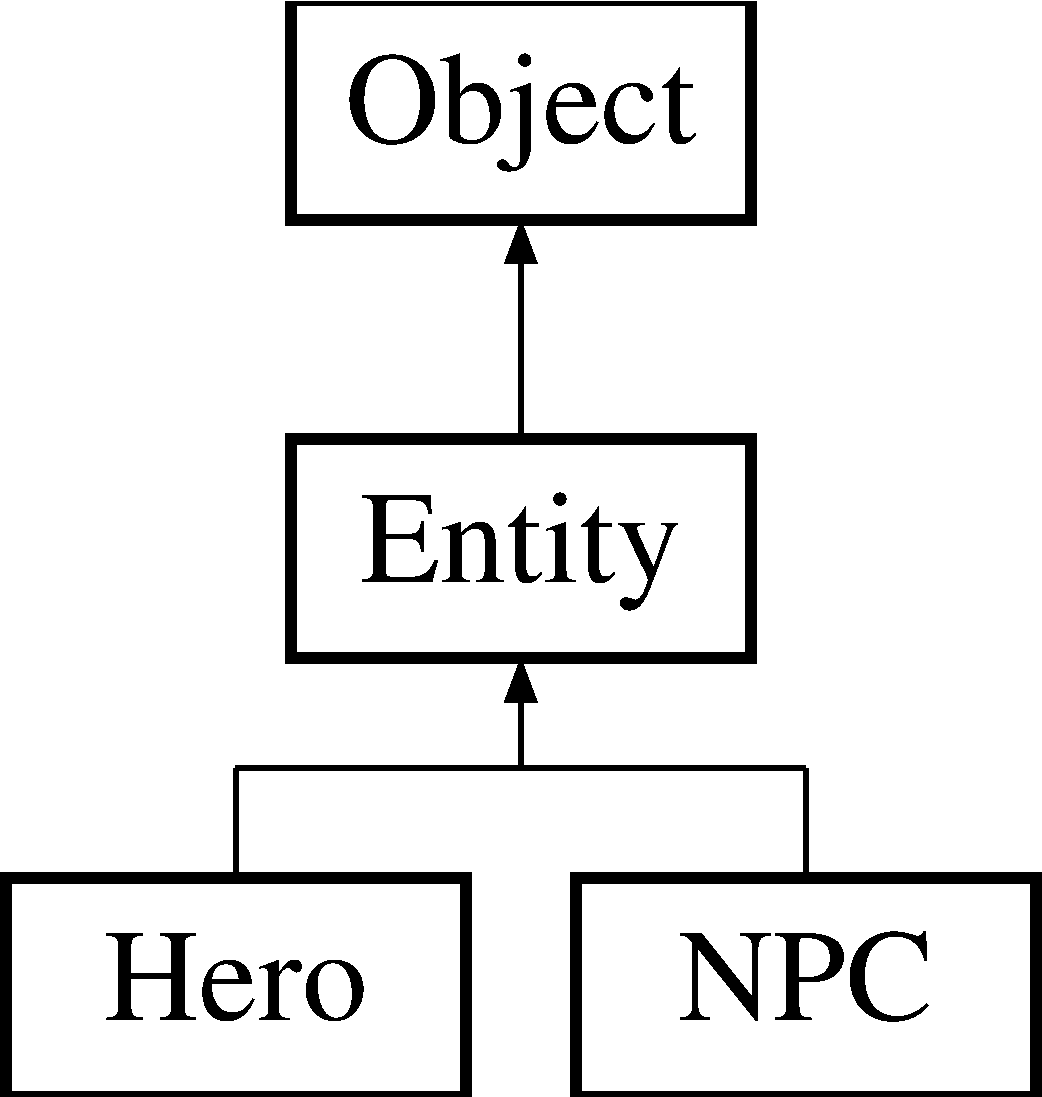
\includegraphics[height=3.000000cm]{class_entity}
\end{center}
\end{figure}
\subsection*{Public Member Functions}
\begin{DoxyCompactItemize}
\item 
\hyperlink{class_entity_adb44f34990023b1802bb95c280d62de0}{Entity} (\hyperlink{class_sprite}{Sprite} $\ast$\hyperlink{class_object_ad936466f3f6b6e8fa401842c573b44e6}{sprite}, float \hyperlink{class_object_a99addca3b5d96c214fa8f90474224699}{x}, float \hyperlink{class_object_a2870044ec214e97550ee28db89c6382a}{y}, char d)
\begin{DoxyCompactList}\small\item\em Deafult constructor. Works just like it would work with an \hyperlink{class_object}{Object}. \end{DoxyCompactList}\item 
\hyperlink{class_entity_adf6d3f7cb1b2ba029b6b048a395cc8ae}{$\sim$\-Entity} ()
\begin{DoxyCompactList}\small\item\em Default destructor. Works just like it would work with an \hyperlink{class_object}{Object}. \end{DoxyCompactList}\item 
bool \hyperlink{class_entity_aac771d739c55a8bf04a40a7d65d849e4}{collides\-On} (char dir)
\begin{DoxyCompactList}\small\item\em Check if a collision is ocurring in any direction. \end{DoxyCompactList}\item 
void \hyperlink{class_entity_a97bff8e950182981a271e548f63fb6c6}{bind\-Joystick} (\hyperlink{class_joystick}{Joystick} $\ast$j)
\begin{DoxyCompactList}\small\item\em Binds a new \hyperlink{class_joystick}{Joystick} instance to the \hyperlink{class_entity}{Entity}. \end{DoxyCompactList}\item 
virtual void \hyperlink{class_entity_a00b6eeaf99b35c8f8b10b5fbfc1baf4f}{update} ()
\begin{DoxyCompactList}\small\item\em Overridable update method. \end{DoxyCompactList}\end{DoxyCompactItemize}
\subsection*{Additional Inherited Members}


\subsection{Detailed Description}
Any \hyperlink{class_object}{Object} that is affected by gravity or capable of random motion. 

Contrary to popular definition, an \hyperlink{class_entity}{Entity} is defined in S2\-M as any type of object (living, mechanic, inanimated) that is capable of being affected by gravity and having random motion at any given time of the game. 

\subsection{Constructor \& Destructor Documentation}
\hypertarget{class_entity_adb44f34990023b1802bb95c280d62de0}{\index{Entity@{Entity}!Entity@{Entity}}
\index{Entity@{Entity}!Entity@{Entity}}
\subsubsection[{Entity}]{\setlength{\rightskip}{0pt plus 5cm}Entity\-::\-Entity (
\begin{DoxyParamCaption}
\item[{{\bf Sprite} $\ast$}]{sprite, }
\item[{float}]{x, }
\item[{float}]{y, }
\item[{char}]{d}
\end{DoxyParamCaption}
)}}\label{class_entity_adb44f34990023b1802bb95c280d62de0}


Deafult constructor. Works just like it would work with an \hyperlink{class_object}{Object}. 

\hypertarget{class_entity_adf6d3f7cb1b2ba029b6b048a395cc8ae}{\index{Entity@{Entity}!$\sim$\-Entity@{$\sim$\-Entity}}
\index{$\sim$\-Entity@{$\sim$\-Entity}!Entity@{Entity}}
\subsubsection[{$\sim$\-Entity}]{\setlength{\rightskip}{0pt plus 5cm}Entity\-::$\sim$\-Entity (
\begin{DoxyParamCaption}
{}
\end{DoxyParamCaption}
)}}\label{class_entity_adf6d3f7cb1b2ba029b6b048a395cc8ae}


Default destructor. Works just like it would work with an \hyperlink{class_object}{Object}. 



\subsection{Member Function Documentation}
\hypertarget{class_entity_a97bff8e950182981a271e548f63fb6c6}{\index{Entity@{Entity}!bind\-Joystick@{bind\-Joystick}}
\index{bind\-Joystick@{bind\-Joystick}!Entity@{Entity}}
\subsubsection[{bind\-Joystick}]{\setlength{\rightskip}{0pt plus 5cm}void Entity\-::bind\-Joystick (
\begin{DoxyParamCaption}
\item[{{\bf Joystick} $\ast$}]{j}
\end{DoxyParamCaption}
)}}\label{class_entity_a97bff8e950182981a271e548f63fb6c6}


Binds a new \hyperlink{class_joystick}{Joystick} instance to the \hyperlink{class_entity}{Entity}. 

\hypertarget{class_entity_aac771d739c55a8bf04a40a7d65d849e4}{\index{Entity@{Entity}!collides\-On@{collides\-On}}
\index{collides\-On@{collides\-On}!Entity@{Entity}}
\subsubsection[{collides\-On}]{\setlength{\rightskip}{0pt plus 5cm}bool Entity\-::collides\-On (
\begin{DoxyParamCaption}
\item[{char}]{dir}
\end{DoxyParamCaption}
)}}\label{class_entity_aac771d739c55a8bf04a40a7d65d849e4}


Check if a collision is ocurring in any direction. 


\begin{DoxyParams}{Parameters}
{\em dir} & the direction to check the collision at. \\
\hline
\end{DoxyParams}
\begin{DoxyReturn}{Returns}
Whether it is ocurring or not 
\end{DoxyReturn}
\hypertarget{class_entity_a00b6eeaf99b35c8f8b10b5fbfc1baf4f}{\index{Entity@{Entity}!update@{update}}
\index{update@{update}!Entity@{Entity}}
\subsubsection[{update}]{\setlength{\rightskip}{0pt plus 5cm}void Entity\-::update (
\begin{DoxyParamCaption}
{}
\end{DoxyParamCaption}
)\hspace{0.3cm}{\ttfamily [virtual]}}}\label{class_entity_a00b6eeaf99b35c8f8b10b5fbfc1baf4f}


Overridable update method. 

If you derive the \hyperlink{class_entity}{Entity} class be sure to place 
\begin{DoxyCode}
\hyperlink{class_entity_a00b6eeaf99b35c8f8b10b5fbfc1baf4f}{Entity::update}();
\end{DoxyCode}
 on the E\-N\-D of the new class' update method so it can implement the \hyperlink{class_entity}{Entity} default update method, which implements \hyperlink{class_object}{Object}'s as well. Default \hyperlink{class_sprite}{Sprite} facing is left, so change this is it's not your case.

When facing left, \hyperlink{}{facing} is equal to false. 

Reimplemented from \hyperlink{class_object_a4abd48bacb1b004c8ac891597c831f77}{Object}.



The documentation for this class was generated from the following files\-:\begin{DoxyCompactItemize}
\item 
src/platformer/\hyperlink{entity_8h}{entity.\-h}\item 
src/platformer/\hyperlink{entity_8cpp}{entity.\-cpp}\end{DoxyCompactItemize}

\hypertarget{class_graphics}{\section{Graphics Class Reference}
\label{class_graphics}\index{Graphics@{Graphics}}
}


Controlls everything graphics-\/related.  




{\ttfamily \#include $<$graphics.\-h$>$}

\subsection*{Public Member Functions}
\begin{DoxyCompactItemize}
\item 
\hyperlink{class_graphics_a6a0d98b9552ff541d543ff5f56759410}{Graphics} (int log\-Width, int log\-Height, string win\-Caption, \hyperlink{class_options}{Options} $\ast$options)
\begin{DoxyCompactList}\small\item\em The constructor. \end{DoxyCompactList}\item 
\hyperlink{class_graphics_a7841c9a961ac9bca33bd30ddf8066cdb}{$\sim$\-Graphics} ()
\begin{DoxyCompactList}\small\item\em The destructor. \end{DoxyCompactList}\item 
S\-D\-L\-\_\-\-Texture $\ast$ \hyperlink{class_graphics_ae584d38c352d13cf792d91bd3b1f2804}{load\-Texture} (string filename, bool drawable)
\begin{DoxyCompactList}\small\item\em Loads a bitmap file and makes it an S\-D\-L\-\_\-\-Texture. \end{DoxyCompactList}\item 
void \hyperlink{class_graphics_abd63e855ce736b83c931a40257741145}{draw\-Texture} (S\-D\-L\-\_\-\-Texture $\ast$source, int x, int y, int w, int h)
\begin{DoxyCompactList}\small\item\em Draws a texture directly on the screen. \end{DoxyCompactList}\item 
void \hyperlink{class_graphics_a84c6ec14161fd77ab529f3f985067df2}{blit\-Texture} (S\-D\-L\-\_\-\-Texture $\ast$tsrc, S\-D\-L\-\_\-\-Texture $\ast$tdest, int x, int y, bool clear)
\begin{DoxyCompactList}\small\item\em Blits a source texture into a destination texture. \end{DoxyCompactList}\item 
void \hyperlink{class_graphics_a2b8441851d9c70e6ae7b3c103f46162d}{blit\-Texture} (S\-D\-L\-\_\-\-Texture $\ast$tsrc, S\-D\-L\-\_\-\-Texture $\ast$tdest, int x, int y, int w, int h, bool clear)
\begin{DoxyCompactList}\small\item\em Blits a source texture into a destination texture. \end{DoxyCompactList}\item 
void \hyperlink{class_graphics_ab3ba379c5c196820b59dcda8fda24db9}{blit\-Texture} (S\-D\-L\-\_\-\-Texture $\ast$tsrc, S\-D\-L\-\_\-\-Texture $\ast$tdest, S\-D\-L\-\_\-\-Rect $\ast$src, S\-D\-L\-\_\-\-Rect $\ast$dest, bool clear)
\begin{DoxyCompactList}\small\item\em Blits a source texture into a destination texture. \end{DoxyCompactList}\item 
void \hyperlink{class_graphics_a5a5297a160c22f73300dcf72ac0be7c2}{update} ()
\begin{DoxyCompactList}\small\item\em Flips the game screen and updates all instantiated Sprites. \end{DoxyCompactList}\item 
void \hyperlink{class_graphics_a398c8e6d13eda586fcfb50952ba25eac}{add\-Sprite} (\hyperlink{class_sprite}{Sprite} $\ast$sprite)
\begin{DoxyCompactList}\small\item\em Adds a \hyperlink{class_sprite}{Sprite} to the \hyperlink{class_graphics_ad01e5a24a1ce34c64f6dd7de4f85fc8b}{sprites} vector. \end{DoxyCompactList}\item 
void \hyperlink{class_graphics_ad06e41bffceda0186291e520fb37fa67}{add\-G\-U\-I\-Element} (\hyperlink{class_g_u_i_element}{G\-U\-I\-Element} $\ast$g)
\begin{DoxyCompactList}\small\item\em Adds a \hyperlink{class_g_u_i_element}{G\-U\-I\-Element} to the \hyperlink{class_graphics_ac4ea71ee39d3cbc7b3fc14bf89fa400f}{guielements} vector. \end{DoxyCompactList}\item 
int \hyperlink{class_graphics_a6364aacb31a2f59c0ad7b423d10a6e3a}{get\-Game\-Width} ()
\begin{DoxyCompactList}\small\item\em Gets the game width. \end{DoxyCompactList}\item 
int \hyperlink{class_graphics_a714496ad1b9244d6f9dafe665b35860d}{get\-Game\-Height} ()
\begin{DoxyCompactList}\small\item\em Gets the game height. \end{DoxyCompactList}\end{DoxyCompactItemize}
\subsection*{Public Attributes}
\begin{DoxyCompactItemize}
\item 
S\-D\-L\-\_\-\-Window $\ast$ \hyperlink{class_graphics_af397f61e26b41302b0b66ee4ab408952}{window}
\begin{DoxyCompactList}\small\item\em The game window S\-D\-L\-\_\-\-Window instance pointer. \end{DoxyCompactList}\item 
S\-D\-L\-\_\-\-Renderer $\ast$ \hyperlink{class_graphics_afee9119ae93eafc5707a9e868b539a2e}{renderer}
\begin{DoxyCompactList}\small\item\em The game renderer S\-D\-L\-\_\-\-Renderer instance pointer. \end{DoxyCompactList}\end{DoxyCompactItemize}
\subsection*{Protected Attributes}
\begin{DoxyCompactItemize}
\item 
int \hyperlink{class_graphics_adf4a36eb3049ba3d07d79af2b4ac6399}{gamewidth}
\begin{DoxyCompactList}\small\item\em The game width. \end{DoxyCompactList}\item 
int \hyperlink{class_graphics_ac176bce8a1a8b73f6ed05e68410d9a14}{gameheight}
\begin{DoxyCompactList}\small\item\em The game height. \end{DoxyCompactList}\item 
S\-D\-L\-\_\-\-Texture $\ast$ \hyperlink{class_graphics_aa3ea5fd0f0a672850bb1352d5ca302f1}{buffer}
\begin{DoxyCompactList}\small\item\em D\-E\-P\-R\-E\-C\-A\-T\-E\-D\-: A buffer to hold the whole screen. \end{DoxyCompactList}\item 
\hyperlink{class_options}{Options} $\ast$ \hyperlink{class_graphics_aafe6ff08323ccbe6478472e3ec30715c}{g\-Options}
\begin{DoxyCompactList}\small\item\em Pointer to the \hyperlink{class_options}{Options} instance. \end{DoxyCompactList}\item 
vector$<$ \hyperlink{class_sprite}{Sprite} $\ast$ $>$ \hyperlink{class_graphics_ad01e5a24a1ce34c64f6dd7de4f85fc8b}{sprites}
\begin{DoxyCompactList}\small\item\em Vector containing every single \hyperlink{class_sprite}{Sprite} that is being used. \end{DoxyCompactList}\item 
vector$<$ \hyperlink{class_g_u_i_element}{G\-U\-I\-Element} $\ast$ $>$ \hyperlink{class_graphics_ac4ea71ee39d3cbc7b3fc14bf89fa400f}{guielements}
\begin{DoxyCompactList}\small\item\em Vector containing every single \hyperlink{class_g_u_i_element}{G\-U\-I\-Element}. \end{DoxyCompactList}\end{DoxyCompactItemize}


\subsection{Detailed Description}
Controlls everything graphics-\/related. 

The \hyperlink{class_graphics}{Graphics} class is an abstraction of everything graphic-\/based in the game. Every operation that involves graphics should need a pointer to this class. 

\subsection{Constructor \& Destructor Documentation}
\hypertarget{class_graphics_a6a0d98b9552ff541d543ff5f56759410}{\index{Graphics@{Graphics}!Graphics@{Graphics}}
\index{Graphics@{Graphics}!Graphics@{Graphics}}
\subsubsection[{Graphics}]{\setlength{\rightskip}{0pt plus 5cm}Graphics\-::\-Graphics (
\begin{DoxyParamCaption}
\item[{int}]{log\-Width, }
\item[{int}]{log\-Height, }
\item[{string}]{win\-Caption, }
\item[{{\bf Options} $\ast$}]{options}
\end{DoxyParamCaption}
)}}\label{class_graphics_a6a0d98b9552ff541d543ff5f56759410}


The constructor. 

Creates a new window and gives it a caption. Uses logical size instead of window size. What this means is that it will create a window based on the size you input times the scaling integer that the \hyperlink{class_options}{Options} instance has, based on what you have specified in the config file. 
\begin{DoxyParams}{Parameters}
{\em win\-Width} & the game width \\
\hline
{\em win\-Height} & the game height \\
\hline
{\em win\-Caption} & the window caption \\
\hline
{\em options} & a pointer to an \hyperlink{class_options}{Options} instance \\
\hline
\end{DoxyParams}
\begin{DoxySeeAlso}{See Also}
\hyperlink{class_graphics_a7841c9a961ac9bca33bd30ddf8066cdb}{$\sim$\-Graphics} 
\end{DoxySeeAlso}
\hypertarget{class_graphics_a7841c9a961ac9bca33bd30ddf8066cdb}{\index{Graphics@{Graphics}!$\sim$\-Graphics@{$\sim$\-Graphics}}
\index{$\sim$\-Graphics@{$\sim$\-Graphics}!Graphics@{Graphics}}
\subsubsection[{$\sim$\-Graphics}]{\setlength{\rightskip}{0pt plus 5cm}Graphics\-::$\sim$\-Graphics (
\begin{DoxyParamCaption}
{}
\end{DoxyParamCaption}
)}}\label{class_graphics_a7841c9a961ac9bca33bd30ddf8066cdb}


The destructor. 

Destroys the current window, frees all existing textures and by all means finishes the game. \begin{DoxySeeAlso}{See Also}
\hyperlink{class_graphics}{Graphics} 
\end{DoxySeeAlso}


\subsection{Member Function Documentation}
\hypertarget{class_graphics_ad06e41bffceda0186291e520fb37fa67}{\index{Graphics@{Graphics}!add\-G\-U\-I\-Element@{add\-G\-U\-I\-Element}}
\index{add\-G\-U\-I\-Element@{add\-G\-U\-I\-Element}!Graphics@{Graphics}}
\subsubsection[{add\-G\-U\-I\-Element}]{\setlength{\rightskip}{0pt plus 5cm}void Graphics\-::add\-G\-U\-I\-Element (
\begin{DoxyParamCaption}
\item[{{\bf G\-U\-I\-Element} $\ast$}]{g}
\end{DoxyParamCaption}
)}}\label{class_graphics_ad06e41bffceda0186291e520fb37fa67}


Adds a \hyperlink{class_g_u_i_element}{G\-U\-I\-Element} to the \hyperlink{class_graphics_ac4ea71ee39d3cbc7b3fc14bf89fa400f}{guielements} vector. 


\begin{DoxyParams}{Parameters}
{\em g} & the \hyperlink{class_g_u_i_element}{G\-U\-I\-Element} to add \\
\hline
\end{DoxyParams}
\hypertarget{class_graphics_a398c8e6d13eda586fcfb50952ba25eac}{\index{Graphics@{Graphics}!add\-Sprite@{add\-Sprite}}
\index{add\-Sprite@{add\-Sprite}!Graphics@{Graphics}}
\subsubsection[{add\-Sprite}]{\setlength{\rightskip}{0pt plus 5cm}void Graphics\-::add\-Sprite (
\begin{DoxyParamCaption}
\item[{{\bf Sprite} $\ast$}]{sprite}
\end{DoxyParamCaption}
)}}\label{class_graphics_a398c8e6d13eda586fcfb50952ba25eac}


Adds a \hyperlink{class_sprite}{Sprite} to the \hyperlink{class_graphics_ad01e5a24a1ce34c64f6dd7de4f85fc8b}{sprites} vector. 


\begin{DoxyParams}{Parameters}
{\em sprite} & the sprite pointer to add \\
\hline
\end{DoxyParams}
\hypertarget{class_graphics_a84c6ec14161fd77ab529f3f985067df2}{\index{Graphics@{Graphics}!blit\-Texture@{blit\-Texture}}
\index{blit\-Texture@{blit\-Texture}!Graphics@{Graphics}}
\subsubsection[{blit\-Texture}]{\setlength{\rightskip}{0pt plus 5cm}void Graphics\-::blit\-Texture (
\begin{DoxyParamCaption}
\item[{S\-D\-L\-\_\-\-Texture $\ast$}]{tsrc, }
\item[{S\-D\-L\-\_\-\-Texture $\ast$}]{tdest, }
\item[{int}]{x, }
\item[{int}]{y, }
\item[{bool}]{clear}
\end{DoxyParamCaption}
)}}\label{class_graphics_a84c6ec14161fd77ab529f3f985067df2}


Blits a source texture into a destination texture. 


\begin{DoxyParams}{Parameters}
{\em tsrc} & the source texture \\
\hline
{\em tdest} & the destination texture \\
\hline
{\em x} & destination horizontal position \\
\hline
{\em y} & destination vertical position \\
\hline
{\em clear} & whether to clear or not the destination texture before blitting \\
\hline
\end{DoxyParams}
\hypertarget{class_graphics_a2b8441851d9c70e6ae7b3c103f46162d}{\index{Graphics@{Graphics}!blit\-Texture@{blit\-Texture}}
\index{blit\-Texture@{blit\-Texture}!Graphics@{Graphics}}
\subsubsection[{blit\-Texture}]{\setlength{\rightskip}{0pt plus 5cm}void Graphics\-::blit\-Texture (
\begin{DoxyParamCaption}
\item[{S\-D\-L\-\_\-\-Texture $\ast$}]{tsrc, }
\item[{S\-D\-L\-\_\-\-Texture $\ast$}]{tdest, }
\item[{int}]{x, }
\item[{int}]{y, }
\item[{int}]{w, }
\item[{int}]{h, }
\item[{bool}]{clear}
\end{DoxyParamCaption}
)}}\label{class_graphics_a2b8441851d9c70e6ae7b3c103f46162d}


Blits a source texture into a destination texture. 

This method lets you scale your texture. 
\begin{DoxyParams}{Parameters}
{\em tsrc} & the source texture \\
\hline
{\em tdest} & the destination texture \\
\hline
{\em x} & destination horizontal position \\
\hline
{\em y} & destination vertical position \\
\hline
{\em w} & width to scale the given texture to \\
\hline
{\em h} & height to scale the given texture to \\
\hline
{\em clear} & whether to clear or not the destination texture before blitting \\
\hline
\end{DoxyParams}
\hypertarget{class_graphics_ab3ba379c5c196820b59dcda8fda24db9}{\index{Graphics@{Graphics}!blit\-Texture@{blit\-Texture}}
\index{blit\-Texture@{blit\-Texture}!Graphics@{Graphics}}
\subsubsection[{blit\-Texture}]{\setlength{\rightskip}{0pt plus 5cm}void Graphics\-::blit\-Texture (
\begin{DoxyParamCaption}
\item[{S\-D\-L\-\_\-\-Texture $\ast$}]{tsrc, }
\item[{S\-D\-L\-\_\-\-Texture $\ast$}]{tdest, }
\item[{S\-D\-L\-\_\-\-Rect $\ast$}]{src, }
\item[{S\-D\-L\-\_\-\-Rect $\ast$}]{dest, }
\item[{bool}]{clear}
\end{DoxyParamCaption}
)}}\label{class_graphics_ab3ba379c5c196820b59dcda8fda24db9}


Blits a source texture into a destination texture. 

This method is a bit more complex but gives you access to cropping and scaling your textures. 
\begin{DoxyParams}{Parameters}
{\em tsrc} & the source texture \\
\hline
{\em tdest} & the destination texture \\
\hline
{\em src} & S\-D\-L\-\_\-\-Rect of the source texture \\
\hline
{\em dest} & S\-D\-L\-\_\-\-Rect of the destination texture \\
\hline
{\em clear} & whether to clear or not the destination texture before blitting \\
\hline
\end{DoxyParams}
\hypertarget{class_graphics_abd63e855ce736b83c931a40257741145}{\index{Graphics@{Graphics}!draw\-Texture@{draw\-Texture}}
\index{draw\-Texture@{draw\-Texture}!Graphics@{Graphics}}
\subsubsection[{draw\-Texture}]{\setlength{\rightskip}{0pt plus 5cm}void Graphics\-::draw\-Texture (
\begin{DoxyParamCaption}
\item[{S\-D\-L\-\_\-\-Texture $\ast$}]{source, }
\item[{int}]{x, }
\item[{int}]{y, }
\item[{int}]{w, }
\item[{int}]{h}
\end{DoxyParamCaption}
)}}\label{class_graphics_abd63e855ce736b83c931a40257741145}


Draws a texture directly on the screen. 

This function draws a texture onscreen, bypassing viewports. 
\begin{DoxyParams}{Parameters}
{\em source} & the texture to blit \\
\hline
{\em x} & horizontal position on screen \\
\hline
{\em y} & vertical position on screen \\
\hline
{\em w} & width to scale the given texture to \\
\hline
{\em h} & height to scale the given texture to \\
\hline
\end{DoxyParams}
\hypertarget{class_graphics_a714496ad1b9244d6f9dafe665b35860d}{\index{Graphics@{Graphics}!get\-Game\-Height@{get\-Game\-Height}}
\index{get\-Game\-Height@{get\-Game\-Height}!Graphics@{Graphics}}
\subsubsection[{get\-Game\-Height}]{\setlength{\rightskip}{0pt plus 5cm}int Graphics\-::get\-Game\-Height (
\begin{DoxyParamCaption}
{}
\end{DoxyParamCaption}
)}}\label{class_graphics_a714496ad1b9244d6f9dafe665b35860d}


Gets the game height. 

\begin{DoxyReturn}{Returns}
The game height. 
\end{DoxyReturn}
\hypertarget{class_graphics_a6364aacb31a2f59c0ad7b423d10a6e3a}{\index{Graphics@{Graphics}!get\-Game\-Width@{get\-Game\-Width}}
\index{get\-Game\-Width@{get\-Game\-Width}!Graphics@{Graphics}}
\subsubsection[{get\-Game\-Width}]{\setlength{\rightskip}{0pt plus 5cm}int Graphics\-::get\-Game\-Width (
\begin{DoxyParamCaption}
{}
\end{DoxyParamCaption}
)}}\label{class_graphics_a6364aacb31a2f59c0ad7b423d10a6e3a}


Gets the game width. 

\begin{DoxyReturn}{Returns}
The game width. 
\end{DoxyReturn}
\hypertarget{class_graphics_ae584d38c352d13cf792d91bd3b1f2804}{\index{Graphics@{Graphics}!load\-Texture@{load\-Texture}}
\index{load\-Texture@{load\-Texture}!Graphics@{Graphics}}
\subsubsection[{load\-Texture}]{\setlength{\rightskip}{0pt plus 5cm}S\-D\-L\-\_\-\-Texture $\ast$ Graphics\-::load\-Texture (
\begin{DoxyParamCaption}
\item[{string}]{filename, }
\item[{bool}]{drawable}
\end{DoxyParamCaption}
)}}\label{class_graphics_ae584d38c352d13cf792d91bd3b1f2804}


Loads a bitmap file and makes it an S\-D\-L\-\_\-\-Texture. 


\begin{DoxyParams}{Parameters}
{\em filename} & the bitmap to load (extension included) \\
\hline
{\em drawable} & indicates if the texture can or cannot be altered over time \\
\hline
\end{DoxyParams}
\begin{DoxyReturn}{Returns}
Pointer to S\-D\-L\-\_\-\-Texture representing the loaded bitmap 
\end{DoxyReturn}
\hypertarget{class_graphics_a5a5297a160c22f73300dcf72ac0be7c2}{\index{Graphics@{Graphics}!update@{update}}
\index{update@{update}!Graphics@{Graphics}}
\subsubsection[{update}]{\setlength{\rightskip}{0pt plus 5cm}void Graphics\-::update (
\begin{DoxyParamCaption}
{}
\end{DoxyParamCaption}
)}}\label{class_graphics_a5a5297a160c22f73300dcf72ac0be7c2}


Flips the game screen and updates all instantiated Sprites. 



\subsection{Member Data Documentation}
\hypertarget{class_graphics_aa3ea5fd0f0a672850bb1352d5ca302f1}{\index{Graphics@{Graphics}!buffer@{buffer}}
\index{buffer@{buffer}!Graphics@{Graphics}}
\subsubsection[{buffer}]{\setlength{\rightskip}{0pt plus 5cm}S\-D\-L\-\_\-\-Texture$\ast$ Graphics\-::buffer\hspace{0.3cm}{\ttfamily [protected]}}}\label{class_graphics_aa3ea5fd0f0a672850bb1352d5ca302f1}


D\-E\-P\-R\-E\-C\-A\-T\-E\-D\-: A buffer to hold the whole screen. 

\hypertarget{class_graphics_ac176bce8a1a8b73f6ed05e68410d9a14}{\index{Graphics@{Graphics}!gameheight@{gameheight}}
\index{gameheight@{gameheight}!Graphics@{Graphics}}
\subsubsection[{gameheight}]{\setlength{\rightskip}{0pt plus 5cm}int Graphics\-::gameheight\hspace{0.3cm}{\ttfamily [protected]}}}\label{class_graphics_ac176bce8a1a8b73f6ed05e68410d9a14}


The game height. 

\hypertarget{class_graphics_adf4a36eb3049ba3d07d79af2b4ac6399}{\index{Graphics@{Graphics}!gamewidth@{gamewidth}}
\index{gamewidth@{gamewidth}!Graphics@{Graphics}}
\subsubsection[{gamewidth}]{\setlength{\rightskip}{0pt plus 5cm}int Graphics\-::gamewidth\hspace{0.3cm}{\ttfamily [protected]}}}\label{class_graphics_adf4a36eb3049ba3d07d79af2b4ac6399}


The game width. 

\hypertarget{class_graphics_aafe6ff08323ccbe6478472e3ec30715c}{\index{Graphics@{Graphics}!g\-Options@{g\-Options}}
\index{g\-Options@{g\-Options}!Graphics@{Graphics}}
\subsubsection[{g\-Options}]{\setlength{\rightskip}{0pt plus 5cm}{\bf Options}$\ast$ Graphics\-::g\-Options\hspace{0.3cm}{\ttfamily [protected]}}}\label{class_graphics_aafe6ff08323ccbe6478472e3ec30715c}


Pointer to the \hyperlink{class_options}{Options} instance. 

\hypertarget{class_graphics_ac4ea71ee39d3cbc7b3fc14bf89fa400f}{\index{Graphics@{Graphics}!guielements@{guielements}}
\index{guielements@{guielements}!Graphics@{Graphics}}
\subsubsection[{guielements}]{\setlength{\rightskip}{0pt plus 5cm}vector$<${\bf G\-U\-I\-Element} $\ast$$>$ Graphics\-::guielements\hspace{0.3cm}{\ttfamily [protected]}}}\label{class_graphics_ac4ea71ee39d3cbc7b3fc14bf89fa400f}


Vector containing every single \hyperlink{class_g_u_i_element}{G\-U\-I\-Element}. 

\hypertarget{class_graphics_afee9119ae93eafc5707a9e868b539a2e}{\index{Graphics@{Graphics}!renderer@{renderer}}
\index{renderer@{renderer}!Graphics@{Graphics}}
\subsubsection[{renderer}]{\setlength{\rightskip}{0pt plus 5cm}S\-D\-L\-\_\-\-Renderer$\ast$ Graphics\-::renderer}}\label{class_graphics_afee9119ae93eafc5707a9e868b539a2e}


The game renderer S\-D\-L\-\_\-\-Renderer instance pointer. 

\hypertarget{class_graphics_ad01e5a24a1ce34c64f6dd7de4f85fc8b}{\index{Graphics@{Graphics}!sprites@{sprites}}
\index{sprites@{sprites}!Graphics@{Graphics}}
\subsubsection[{sprites}]{\setlength{\rightskip}{0pt plus 5cm}vector$<${\bf Sprite} $\ast$$>$ Graphics\-::sprites\hspace{0.3cm}{\ttfamily [protected]}}}\label{class_graphics_ad01e5a24a1ce34c64f6dd7de4f85fc8b}


Vector containing every single \hyperlink{class_sprite}{Sprite} that is being used. 

\hypertarget{class_graphics_af397f61e26b41302b0b66ee4ab408952}{\index{Graphics@{Graphics}!window@{window}}
\index{window@{window}!Graphics@{Graphics}}
\subsubsection[{window}]{\setlength{\rightskip}{0pt plus 5cm}S\-D\-L\-\_\-\-Window$\ast$ Graphics\-::window}}\label{class_graphics_af397f61e26b41302b0b66ee4ab408952}


The game window S\-D\-L\-\_\-\-Window instance pointer. 



The documentation for this class was generated from the following files\-:\begin{DoxyCompactItemize}
\item 
src/\hyperlink{graphics_8h}{graphics.\-h}\item 
src/\hyperlink{graphics_8cpp}{graphics.\-cpp}\end{DoxyCompactItemize}

\hypertarget{class_g_u_i_element}{\section{G\-U\-I\-Element Class Reference}
\label{class_g_u_i_element}\index{G\-U\-I\-Element@{G\-U\-I\-Element}}
}


A separate element of the G\-U\-I that stays on top of the game.  




{\ttfamily \#include $<$gui.\-h$>$}

\subsection*{Public Member Functions}
\begin{DoxyCompactItemize}
\item 
\hyperlink{class_g_u_i_element_afef4e7a36240156f714dcbadd5d0d825}{G\-U\-I\-Element} ()
\item 
\hyperlink{class_g_u_i_element_a96d6728fa2a9e92a5a0fe6481dfcae15}{$\sim$\-G\-U\-I\-Element} ()
\item 
virtual void \hyperlink{class_g_u_i_element_a2a7207926c6b55dfd0336d86899d8f92}{draw} ()
\end{DoxyCompactItemize}
\subsection*{Protected Attributes}
\begin{DoxyCompactItemize}
\item 
float \hyperlink{class_g_u_i_element_a7d5e8a612605a3ed7cfd11895a91e6ef}{x}
\begin{DoxyCompactList}\small\item\em Position in the window. \end{DoxyCompactList}\item 
float \hyperlink{class_g_u_i_element_a9415b77e6e60981d2be4a39fdd873cf7}{y}
\item 
bool \hyperlink{class_g_u_i_element_a9385814f8643bdb096013a3846c2516b}{visible} = true
\begin{DoxyCompactList}\small\item\em Determines wether this \hyperlink{class_g_u_i_element}{G\-U\-I\-Element} is currently visible onscreen. \end{DoxyCompactList}\end{DoxyCompactItemize}


\subsection{Detailed Description}
A separate element of the G\-U\-I that stays on top of the game. 

May be a health bar, or the score meter, or some text, whatever. 

\subsection{Constructor \& Destructor Documentation}
\hypertarget{class_g_u_i_element_afef4e7a36240156f714dcbadd5d0d825}{\index{G\-U\-I\-Element@{G\-U\-I\-Element}!G\-U\-I\-Element@{G\-U\-I\-Element}}
\index{G\-U\-I\-Element@{G\-U\-I\-Element}!GUIElement@{G\-U\-I\-Element}}
\subsubsection[{G\-U\-I\-Element}]{\setlength{\rightskip}{0pt plus 5cm}G\-U\-I\-Element\-::\-G\-U\-I\-Element (
\begin{DoxyParamCaption}
{}
\end{DoxyParamCaption}
)}}\label{class_g_u_i_element_afef4e7a36240156f714dcbadd5d0d825}
\hypertarget{class_g_u_i_element_a96d6728fa2a9e92a5a0fe6481dfcae15}{\index{G\-U\-I\-Element@{G\-U\-I\-Element}!$\sim$\-G\-U\-I\-Element@{$\sim$\-G\-U\-I\-Element}}
\index{$\sim$\-G\-U\-I\-Element@{$\sim$\-G\-U\-I\-Element}!GUIElement@{G\-U\-I\-Element}}
\subsubsection[{$\sim$\-G\-U\-I\-Element}]{\setlength{\rightskip}{0pt plus 5cm}G\-U\-I\-Element\-::$\sim$\-G\-U\-I\-Element (
\begin{DoxyParamCaption}
{}
\end{DoxyParamCaption}
)}}\label{class_g_u_i_element_a96d6728fa2a9e92a5a0fe6481dfcae15}


\subsection{Member Function Documentation}
\hypertarget{class_g_u_i_element_a2a7207926c6b55dfd0336d86899d8f92}{\index{G\-U\-I\-Element@{G\-U\-I\-Element}!draw@{draw}}
\index{draw@{draw}!GUIElement@{G\-U\-I\-Element}}
\subsubsection[{draw}]{\setlength{\rightskip}{0pt plus 5cm}void G\-U\-I\-Element\-::draw (
\begin{DoxyParamCaption}
{}
\end{DoxyParamCaption}
)\hspace{0.3cm}{\ttfamily [virtual]}}}\label{class_g_u_i_element_a2a7207926c6b55dfd0336d86899d8f92}


\subsection{Member Data Documentation}
\hypertarget{class_g_u_i_element_a9385814f8643bdb096013a3846c2516b}{\index{G\-U\-I\-Element@{G\-U\-I\-Element}!visible@{visible}}
\index{visible@{visible}!GUIElement@{G\-U\-I\-Element}}
\subsubsection[{visible}]{\setlength{\rightskip}{0pt plus 5cm}bool G\-U\-I\-Element\-::visible = true\hspace{0.3cm}{\ttfamily [protected]}}}\label{class_g_u_i_element_a9385814f8643bdb096013a3846c2516b}


Determines wether this \hyperlink{class_g_u_i_element}{G\-U\-I\-Element} is currently visible onscreen. 

\hypertarget{class_g_u_i_element_a7d5e8a612605a3ed7cfd11895a91e6ef}{\index{G\-U\-I\-Element@{G\-U\-I\-Element}!x@{x}}
\index{x@{x}!GUIElement@{G\-U\-I\-Element}}
\subsubsection[{x}]{\setlength{\rightskip}{0pt plus 5cm}float G\-U\-I\-Element\-::x\hspace{0.3cm}{\ttfamily [protected]}}}\label{class_g_u_i_element_a7d5e8a612605a3ed7cfd11895a91e6ef}


Position in the window. 

\hypertarget{class_g_u_i_element_a9415b77e6e60981d2be4a39fdd873cf7}{\index{G\-U\-I\-Element@{G\-U\-I\-Element}!y@{y}}
\index{y@{y}!GUIElement@{G\-U\-I\-Element}}
\subsubsection[{y}]{\setlength{\rightskip}{0pt plus 5cm}float G\-U\-I\-Element\-::y\hspace{0.3cm}{\ttfamily [protected]}}}\label{class_g_u_i_element_a9415b77e6e60981d2be4a39fdd873cf7}


The documentation for this class was generated from the following files\-:\begin{DoxyCompactItemize}
\item 
src/\hyperlink{gui_8h}{gui.\-h}\item 
src/\hyperlink{gui_8cpp}{gui.\-cpp}\end{DoxyCompactItemize}

\hypertarget{class_hero}{\section{Hero Class Reference}
\label{class_hero}\index{Hero@{Hero}}
}


An \hyperlink{class_entity}{Entity} that can be controlled directly with user input.  




{\ttfamily \#include $<$entity.\-h$>$}

Inheritance diagram for Hero\-:\begin{figure}[H]
\begin{center}
\leavevmode
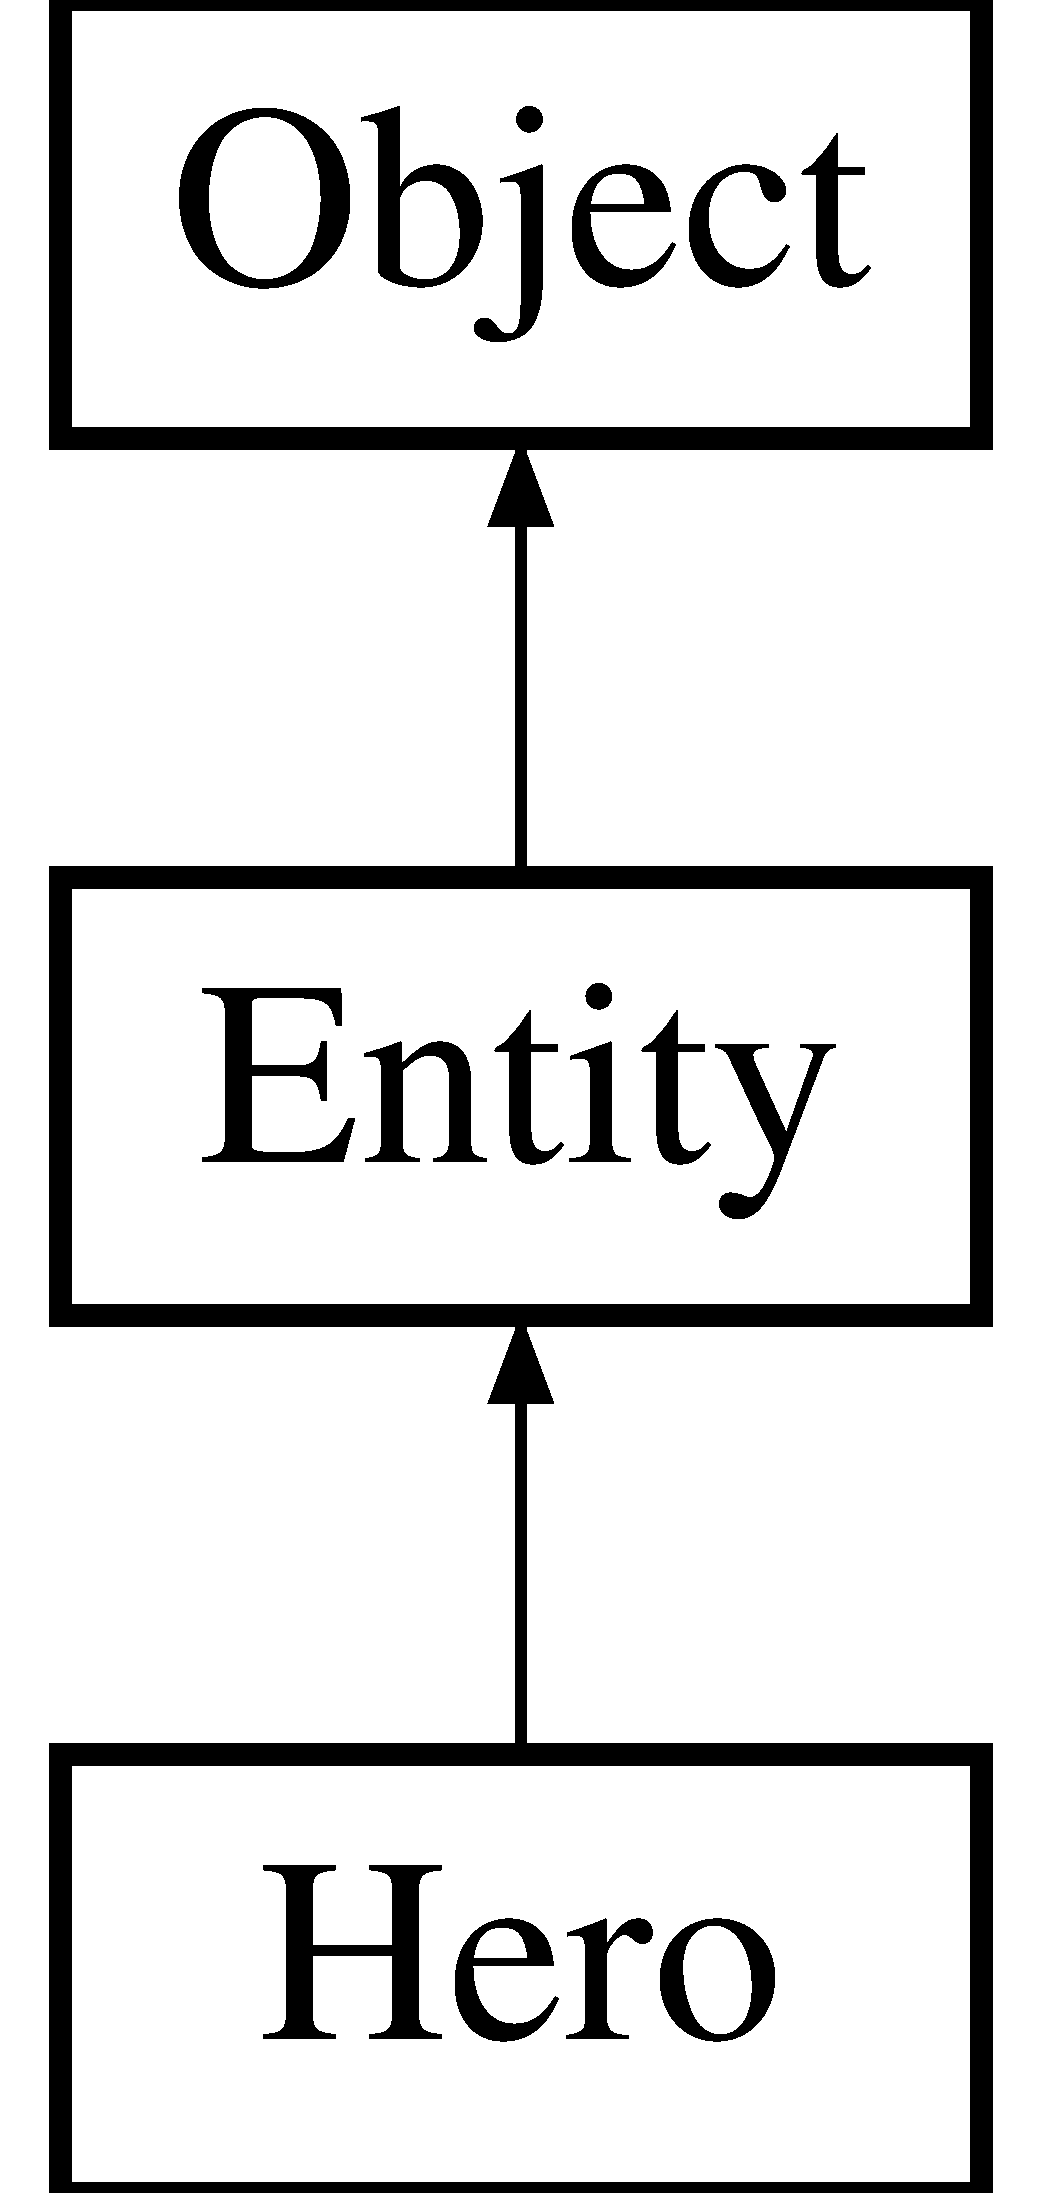
\includegraphics[height=3.000000cm]{class_hero}
\end{center}
\end{figure}
\subsection*{Additional Inherited Members}


\subsection{Detailed Description}
An \hyperlink{class_entity}{Entity} that can be controlled directly with user input. 

A \hyperlink{class_hero}{Hero} is a type of \hyperlink{class_entity}{Entity} that can be controlled with an assigned \hyperlink{class_joystick}{Joystick}. The default assigned \hyperlink{class_joystick}{Joystick} is \hyperlink{joystick_8h_af086526cf25607f16a7940bc163126b1}{g\-Joystick}, but you can assign any other \hyperlink{class_virtual_joystick}{Virtual\-Joystick} if you want your \hyperlink{class_hero}{Hero}'s movement to be script/code-\/determined. 

The documentation for this class was generated from the following file\-:\begin{DoxyCompactItemize}
\item 
src/platformer/\hyperlink{entity_8h}{entity.\-h}\end{DoxyCompactItemize}

\hypertarget{class_joystick}{\section{Joystick Class Reference}
\label{class_joystick}\index{Joystick@{Joystick}}
}


Representation of game buttons/keys.  




{\ttfamily \#include $<$joystick.\-h$>$}

Inheritance diagram for Joystick\-:\begin{figure}[H]
\begin{center}
\leavevmode
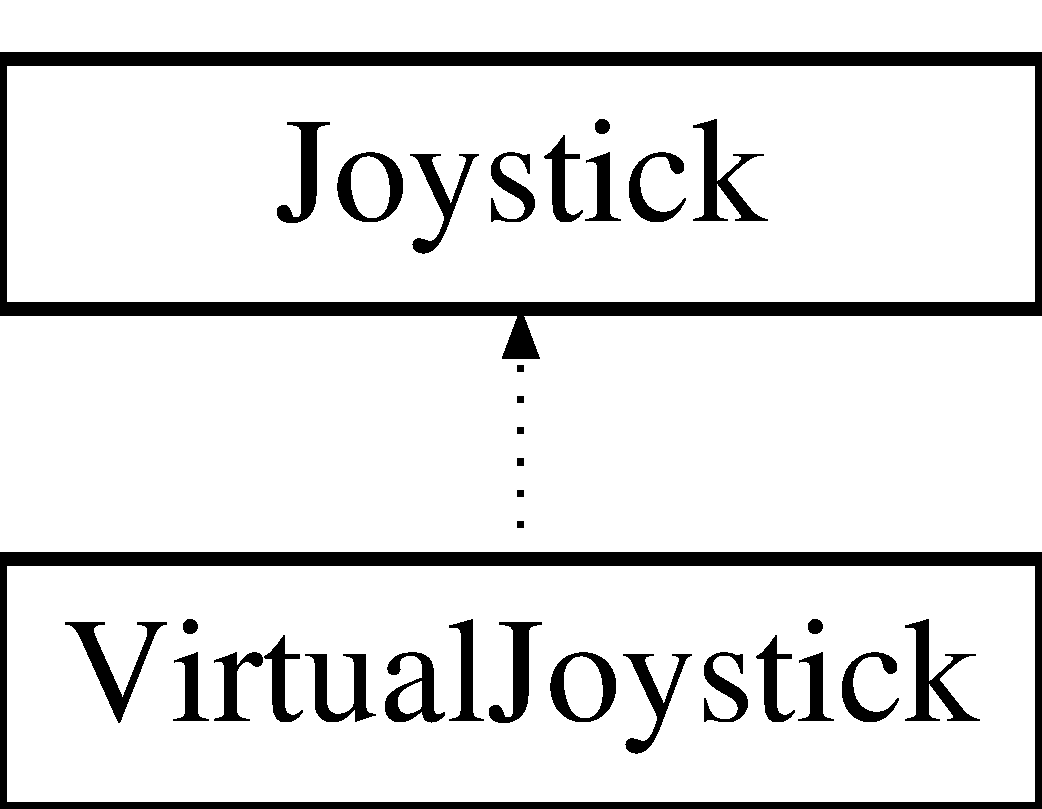
\includegraphics[height=2.000000cm]{class_joystick}
\end{center}
\end{figure}
\subsection*{Public Member Functions}
\begin{DoxyCompactItemize}
\item 
\hyperlink{class_joystick_a158b1f77b78717efbf1b8fac43b1fcef}{Joystick} ()
\item 
bool \hyperlink{class_joystick_aceddfa0d39a5a6f7041c2951cb628060}{get\-Dir} (int i)
\item 
bool \hyperlink{class_joystick_a3a2c6a02979cd631a28f8ab7a5724fdb}{get\-Btn} (int i)
\item 
bool \hyperlink{class_joystick_a726d84c93e26cea55c8e4b2235a13e7e}{get\-Dir\-Pressed} (int i)
\item 
bool \hyperlink{class_joystick_a79399f1438c2ef54e5d8dd0ca59a2433}{get\-Btn\-Pressed} (int i)
\item 
void \hyperlink{class_joystick_a3c3fc5aa1a5482c172fa20f9661a9149}{update} ()
\end{DoxyCompactItemize}


\subsection{Detailed Description}
Representation of game buttons/keys. 

A \hyperlink{class_joystick}{Joystick} is a representation of the game buttons. It is useful if we bond it to a \hyperlink{class_hero}{Hero} instance\-: then it will follow the user's input. When we bond a \hyperlink{class_virtual_joystick}{Virtual\-Joystick} to a \hyperlink{class_hero}{Hero} it will stop following our input and start following game compiled (or scripted) directives. 

\subsection{Constructor \& Destructor Documentation}
\hypertarget{class_joystick_a158b1f77b78717efbf1b8fac43b1fcef}{\index{Joystick@{Joystick}!Joystick@{Joystick}}
\index{Joystick@{Joystick}!Joystick@{Joystick}}
\subsubsection[{Joystick}]{\setlength{\rightskip}{0pt plus 5cm}Joystick\-::\-Joystick (
\begin{DoxyParamCaption}
{}
\end{DoxyParamCaption}
)}}\label{class_joystick_a158b1f77b78717efbf1b8fac43b1fcef}


\subsection{Member Function Documentation}
\hypertarget{class_joystick_a3a2c6a02979cd631a28f8ab7a5724fdb}{\index{Joystick@{Joystick}!get\-Btn@{get\-Btn}}
\index{get\-Btn@{get\-Btn}!Joystick@{Joystick}}
\subsubsection[{get\-Btn}]{\setlength{\rightskip}{0pt plus 5cm}bool Joystick\-::get\-Btn (
\begin{DoxyParamCaption}
\item[{int}]{i}
\end{DoxyParamCaption}
)}}\label{class_joystick_a3a2c6a02979cd631a28f8ab7a5724fdb}
\hypertarget{class_joystick_a79399f1438c2ef54e5d8dd0ca59a2433}{\index{Joystick@{Joystick}!get\-Btn\-Pressed@{get\-Btn\-Pressed}}
\index{get\-Btn\-Pressed@{get\-Btn\-Pressed}!Joystick@{Joystick}}
\subsubsection[{get\-Btn\-Pressed}]{\setlength{\rightskip}{0pt plus 5cm}bool Joystick\-::get\-Btn\-Pressed (
\begin{DoxyParamCaption}
\item[{int}]{i}
\end{DoxyParamCaption}
)}}\label{class_joystick_a79399f1438c2ef54e5d8dd0ca59a2433}
\hypertarget{class_joystick_aceddfa0d39a5a6f7041c2951cb628060}{\index{Joystick@{Joystick}!get\-Dir@{get\-Dir}}
\index{get\-Dir@{get\-Dir}!Joystick@{Joystick}}
\subsubsection[{get\-Dir}]{\setlength{\rightskip}{0pt plus 5cm}bool Joystick\-::get\-Dir (
\begin{DoxyParamCaption}
\item[{int}]{i}
\end{DoxyParamCaption}
)}}\label{class_joystick_aceddfa0d39a5a6f7041c2951cb628060}
\hypertarget{class_joystick_a726d84c93e26cea55c8e4b2235a13e7e}{\index{Joystick@{Joystick}!get\-Dir\-Pressed@{get\-Dir\-Pressed}}
\index{get\-Dir\-Pressed@{get\-Dir\-Pressed}!Joystick@{Joystick}}
\subsubsection[{get\-Dir\-Pressed}]{\setlength{\rightskip}{0pt plus 5cm}bool Joystick\-::get\-Dir\-Pressed (
\begin{DoxyParamCaption}
\item[{int}]{i}
\end{DoxyParamCaption}
)}}\label{class_joystick_a726d84c93e26cea55c8e4b2235a13e7e}
\hypertarget{class_joystick_a3c3fc5aa1a5482c172fa20f9661a9149}{\index{Joystick@{Joystick}!update@{update}}
\index{update@{update}!Joystick@{Joystick}}
\subsubsection[{update}]{\setlength{\rightskip}{0pt plus 5cm}void Joystick\-::update (
\begin{DoxyParamCaption}
{}
\end{DoxyParamCaption}
)}}\label{class_joystick_a3c3fc5aa1a5482c172fa20f9661a9149}


The documentation for this class was generated from the following files\-:\begin{DoxyCompactItemize}
\item 
src/\hyperlink{joystick_8h}{joystick.\-h}\item 
src/\hyperlink{joystick_8cpp}{joystick.\-cpp}\end{DoxyCompactItemize}

\hypertarget{class_n_p_c}{\section{N\-P\-C Class Reference}
\label{class_n_p_c}\index{N\-P\-C@{N\-P\-C}}
}


An \hyperlink{class_entity}{Entity} that can't be directly controlled with user input.  




{\ttfamily \#include $<$entity.\-h$>$}

Inheritance diagram for N\-P\-C\-:\begin{figure}[H]
\begin{center}
\leavevmode
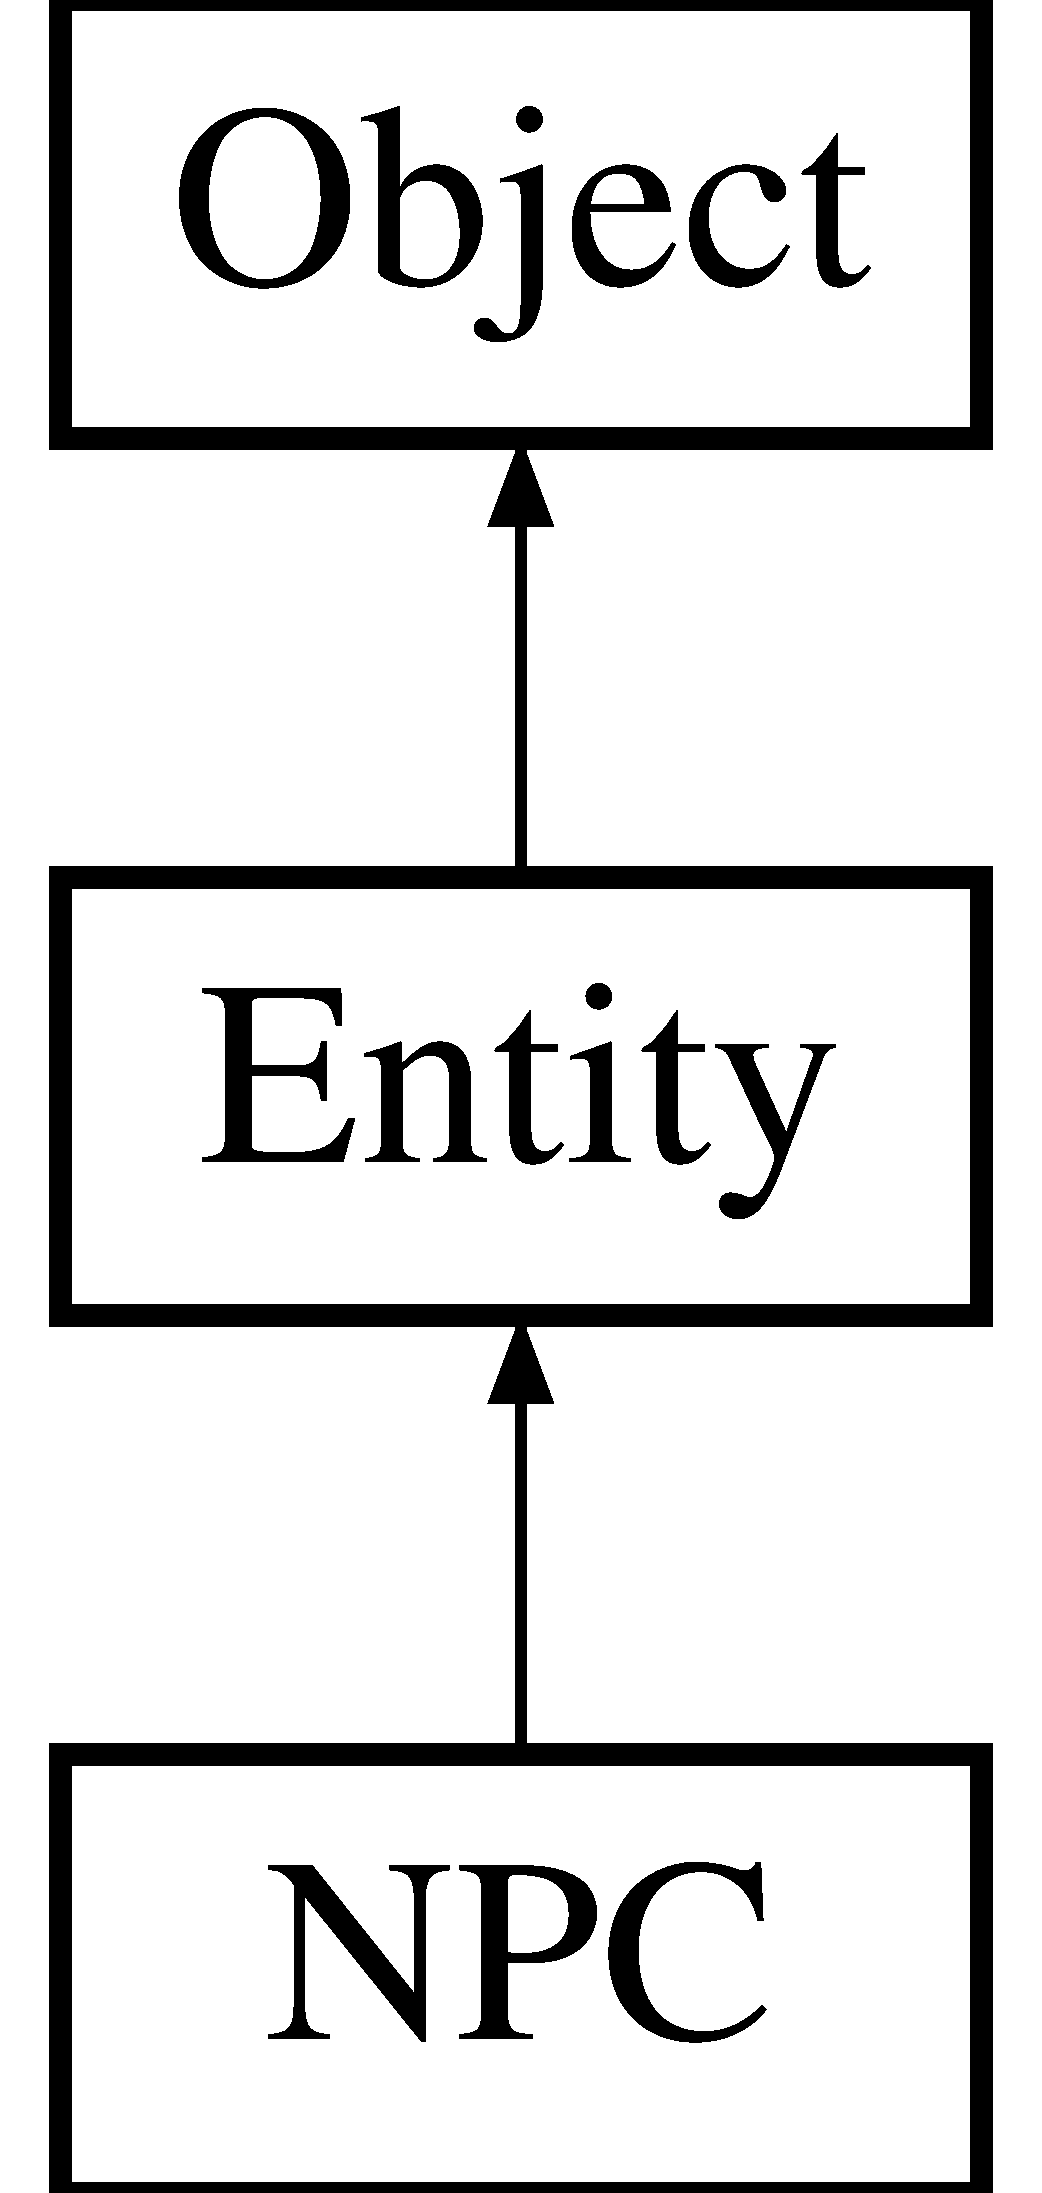
\includegraphics[height=3.000000cm]{class_n_p_c}
\end{center}
\end{figure}
\subsection*{Additional Inherited Members}


\subsection{Detailed Description}
An \hyperlink{class_entity}{Entity} that can't be directly controlled with user input. 

The documentation for this class was generated from the following file\-:\begin{DoxyCompactItemize}
\item 
src/platformer/\hyperlink{entity_8h}{entity.\-h}\end{DoxyCompactItemize}

\hypertarget{class_object}{\section{Object Class Reference}
\label{class_object}\index{Object@{Object}}
}


Anything that can be positioned within a \hyperlink{class_room}{Room}.  




{\ttfamily \#include $<$object.\-h$>$}

Inheritance diagram for Object\-:\begin{figure}[H]
\begin{center}
\leavevmode
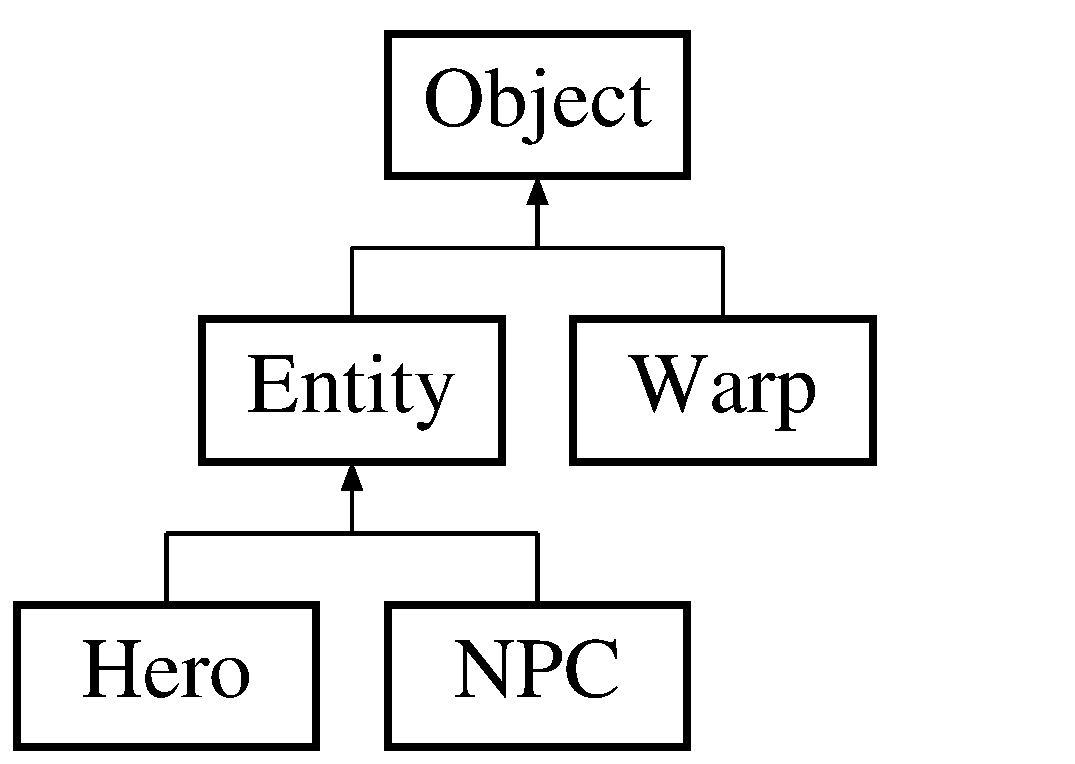
\includegraphics[height=3.000000cm]{class_object}
\end{center}
\end{figure}
\subsection*{Public Member Functions}
\begin{DoxyCompactItemize}
\item 
\hyperlink{class_object_a9e5569564089c40dbfa85703035ddaf2}{Object} (\hyperlink{class_sprite}{Sprite} $\ast$\hyperlink{class_object_ad936466f3f6b6e8fa401842c573b44e6}{sprite}, float \hyperlink{class_object_a99addca3b5d96c214fa8f90474224699}{x}, float \hyperlink{class_object_a2870044ec214e97550ee28db89c6382a}{y}, char d)
\begin{DoxyCompactList}\small\item\em Default constructor. \end{DoxyCompactList}\item 
\hyperlink{class_object_ae8f5483f459e46687bd01e6f9977afd3}{$\sim$\-Object} ()
\begin{DoxyCompactList}\small\item\em Default destructor. \end{DoxyCompactList}\item 
void \hyperlink{class_object_a182782f2325980f649409507c2970af8}{set\-Animation} (int i)
\begin{DoxyCompactList}\small\item\em Sets the current animation. \end{DoxyCompactList}\item 
int \hyperlink{class_object_ab58cde576bd8ae773fa742f147a792f2}{get\-Animation} ()
\begin{DoxyCompactList}\small\item\em Gets the current animation number. \end{DoxyCompactList}\item 
void \hyperlink{class_object_a21d5b472e193c2665cd06be4a9cc270d}{set\-Frame} (int i)
\begin{DoxyCompactList}\small\item\em Sets the current sprite's frame and stops the current animation. \end{DoxyCompactList}\item 
int \hyperlink{class_object_a2a1724269f3d7ebf7007d079312cb850}{get\-Frame} ()
\begin{DoxyCompactList}\small\item\em Gets the current frame number of the \hyperlink{class_sprite}{Sprite}. \end{DoxyCompactList}\item 
void \hyperlink{class_object_a7d97667046ee84c23f4f362892bf4e33}{set\-Depth} (char d)
\begin{DoxyCompactList}\small\item\em Sets the \hyperlink{class_object}{Object}'s depth on the \hyperlink{class_room}{Room}. \end{DoxyCompactList}\item 
char \hyperlink{class_object_aad6045382d08dc0bf4fc8a35915560ea}{get\-Depth} ()
\begin{DoxyCompactList}\small\item\em Gets the \hyperlink{class_object}{Object}'s depth on the \hyperlink{class_room}{Room}. \end{DoxyCompactList}\item 
float \hyperlink{class_object_a9397ff68bd3fdba963dfb054ea5e62c1}{get\-Next\-X} ()
\begin{DoxyCompactList}\small\item\em Get the object's horizontal position on the next frame. \end{DoxyCompactList}\item 
float \hyperlink{class_object_afda996a7119562f31a67e85029567ba7}{get\-Next\-Y} ()
\begin{DoxyCompactList}\small\item\em Get the object's vertical position on the next frame. \end{DoxyCompactList}\item 
virtual void \hyperlink{class_object_a4abd48bacb1b004c8ac891597c831f77}{update} ()
\begin{DoxyCompactList}\small\item\em Overridable update method. You'll need it. \end{DoxyCompactList}\end{DoxyCompactItemize}
\subsection*{Public Attributes}
\begin{DoxyCompactItemize}
\item 
float \hyperlink{class_object_a99addca3b5d96c214fa8f90474224699}{x}
\begin{DoxyCompactList}\small\item\em Horizontal position on the \hyperlink{class_room}{Room}. \end{DoxyCompactList}\item 
float \hyperlink{class_object_a2870044ec214e97550ee28db89c6382a}{y}
\begin{DoxyCompactList}\small\item\em Vertical position on the \hyperlink{class_room}{Room}. \end{DoxyCompactList}\item 
\hyperlink{class_sprite}{Sprite} $\ast$ \hyperlink{class_object_ad936466f3f6b6e8fa401842c573b44e6}{sprite}
\begin{DoxyCompactList}\small\item\em Current \hyperlink{class_sprite}{Sprite} pointer. \end{DoxyCompactList}\end{DoxyCompactItemize}
\subsection*{Protected Attributes}
\begin{DoxyCompactItemize}
\item 
float \hyperlink{class_object_adf988f967e46c4fd5d3276778d83b51c}{xnext}
\begin{DoxyCompactList}\small\item\em Next frame's horizontal position on the \hyperlink{class_room}{Room}. \end{DoxyCompactList}\item 
float \hyperlink{class_object_a23acb9460963396dc0bda8d9dc0c6771}{ynext}
\begin{DoxyCompactList}\small\item\em Next frame's vertical position on the \hyperlink{class_room}{Room}. \end{DoxyCompactList}\item 
int \hyperlink{class_object_afc05c8f84fe3feb003332413f1e5ef75}{spr\-Default\-Frame} = 0
\item 
int \hyperlink{class_object_a671da7bcaade0763ea158d70137017a0}{animation\-Frame} = 0
\item 
int \hyperlink{class_object_ad61c7c0c72c28dd4abbc5f14cfdf3f18}{spr\-Frame} = 0
\item 
int \hyperlink{class_object_a72bd9c2d466c47f6cd8df5e38185d432}{spr\-Animation} = -\/1
\item 
int \hyperlink{class_object_ab66e9611429a7f5a0f0889332514e607}{spr\-Speed}
\item 
int \hyperlink{class_object_aa16902b53e4e950380464c71f0b9554b}{spr\-Speed\-Counter} = 0
\item 
double \hyperlink{class_object_a5e5f645424be8ec1ce1cf9dd858e939a}{spr\-Angle} = 0
\begin{DoxyCompactList}\small\item\em Defines a rotation for the \hyperlink{class_object}{Object}'s \hyperlink{class_sprite}{Sprite}. \end{DoxyCompactList}\item 
S\-D\-L\-\_\-\-Point \hyperlink{class_object_ab5d3b1e8dbb35e139a3fd3a3b28b8610}{spr\-Center}
\begin{DoxyCompactList}\small\item\em Rotating center point. By default it is the \hyperlink{class_sprite}{Sprite}'s center. \end{DoxyCompactList}\item 
S\-D\-L\-\_\-\-Renderer\-Flip \hyperlink{class_object_a1b77d0f13f96d477047be48ae41fb3ea}{spr\-Flip} = S\-D\-L\-\_\-\-F\-L\-I\-P\-\_\-\-N\-O\-N\-E
\begin{DoxyCompactList}\small\item\em Flipping flags for the \hyperlink{class_object}{Object}'s \hyperlink{class_sprite}{Sprite}. \end{DoxyCompactList}\item 
char \hyperlink{class_object_ac02426a63de0baa3b1761925793ea1cf}{depth}
\begin{DoxyCompactList}\small\item\em Default object's depth on screen. \end{DoxyCompactList}\item 
S\-D\-L\-\_\-\-Rect \hyperlink{class_object_ac2bf39eb033cf8c8fc9220d607842dbe}{rect}
\begin{DoxyCompactList}\small\item\em Default S\-D\-L\-\_\-\-Rect. \end{DoxyCompactList}\end{DoxyCompactItemize}
\subsection*{Friends}
\begin{DoxyCompactItemize}
\item 
class \hyperlink{class_object_ae5cfe0c0e0b06d536d5814bd1ff4818f}{Graphics}
\item 
void \hyperlink{class_object_aafd680b61e1b56b735697937b05bf5c7}{Room\-::update} ()
\end{DoxyCompactItemize}


\subsection{Detailed Description}
Anything that can be positioned within a \hyperlink{class_room}{Room}. 

As long as it has x and y coordinates it can be considered an object. 

\subsection{Constructor \& Destructor Documentation}
\hypertarget{class_object_a9e5569564089c40dbfa85703035ddaf2}{\index{Object@{Object}!Object@{Object}}
\index{Object@{Object}!Object@{Object}}
\subsubsection[{Object}]{\setlength{\rightskip}{0pt plus 5cm}Object\-::\-Object (
\begin{DoxyParamCaption}
\item[{{\bf Sprite} $\ast$}]{sprite, }
\item[{float}]{x, }
\item[{float}]{y, }
\item[{char}]{d}
\end{DoxyParamCaption}
)}}\label{class_object_a9e5569564089c40dbfa85703035ddaf2}


Default constructor. 


\begin{DoxyParams}{Parameters}
{\em sprite} & the \hyperlink{class_sprite}{Sprite} the \hyperlink{class_object}{Object}'s gonna use \\
\hline
{\em x} & horizontal position on the \hyperlink{class_room}{Room} \\
\hline
{\em y} & vertical position on the \hyperlink{class_room}{Room} \\
\hline
{\em d} & depth on the \hyperlink{class_room}{Room}, the higher the furthest away \\
\hline
\end{DoxyParams}
\hypertarget{class_object_ae8f5483f459e46687bd01e6f9977afd3}{\index{Object@{Object}!$\sim$\-Object@{$\sim$\-Object}}
\index{$\sim$\-Object@{$\sim$\-Object}!Object@{Object}}
\subsubsection[{$\sim$\-Object}]{\setlength{\rightskip}{0pt plus 5cm}Object\-::$\sim$\-Object (
\begin{DoxyParamCaption}
{}
\end{DoxyParamCaption}
)}}\label{class_object_ae8f5483f459e46687bd01e6f9977afd3}


Default destructor. 



\subsection{Member Function Documentation}
\hypertarget{class_object_ab58cde576bd8ae773fa742f147a792f2}{\index{Object@{Object}!get\-Animation@{get\-Animation}}
\index{get\-Animation@{get\-Animation}!Object@{Object}}
\subsubsection[{get\-Animation}]{\setlength{\rightskip}{0pt plus 5cm}int Object\-::get\-Animation (
\begin{DoxyParamCaption}
{}
\end{DoxyParamCaption}
)}}\label{class_object_ab58cde576bd8ae773fa742f147a792f2}


Gets the current animation number. 

\begin{DoxyReturn}{Returns}
The current animation number. 
\end{DoxyReturn}
\hypertarget{class_object_aad6045382d08dc0bf4fc8a35915560ea}{\index{Object@{Object}!get\-Depth@{get\-Depth}}
\index{get\-Depth@{get\-Depth}!Object@{Object}}
\subsubsection[{get\-Depth}]{\setlength{\rightskip}{0pt plus 5cm}char Object\-::get\-Depth (
\begin{DoxyParamCaption}
{}
\end{DoxyParamCaption}
)}}\label{class_object_aad6045382d08dc0bf4fc8a35915560ea}


Gets the \hyperlink{class_object}{Object}'s depth on the \hyperlink{class_room}{Room}. 

\begin{DoxyReturn}{Returns}
The \hyperlink{class_object}{Object}'s depth on the \hyperlink{class_room}{Room}. 
\end{DoxyReturn}
\hypertarget{class_object_a2a1724269f3d7ebf7007d079312cb850}{\index{Object@{Object}!get\-Frame@{get\-Frame}}
\index{get\-Frame@{get\-Frame}!Object@{Object}}
\subsubsection[{get\-Frame}]{\setlength{\rightskip}{0pt plus 5cm}int Object\-::get\-Frame (
\begin{DoxyParamCaption}
{}
\end{DoxyParamCaption}
)}}\label{class_object_a2a1724269f3d7ebf7007d079312cb850}


Gets the current frame number of the \hyperlink{class_sprite}{Sprite}. 

\begin{DoxyReturn}{Returns}
The current image number. 
\end{DoxyReturn}
\hypertarget{class_object_a9397ff68bd3fdba963dfb054ea5e62c1}{\index{Object@{Object}!get\-Next\-X@{get\-Next\-X}}
\index{get\-Next\-X@{get\-Next\-X}!Object@{Object}}
\subsubsection[{get\-Next\-X}]{\setlength{\rightskip}{0pt plus 5cm}float Object\-::get\-Next\-X (
\begin{DoxyParamCaption}
{}
\end{DoxyParamCaption}
)}}\label{class_object_a9397ff68bd3fdba963dfb054ea5e62c1}


Get the object's horizontal position on the next frame. 

\begin{DoxyReturn}{Returns}
The object's horizontal position on the next frame. 
\end{DoxyReturn}
\hypertarget{class_object_afda996a7119562f31a67e85029567ba7}{\index{Object@{Object}!get\-Next\-Y@{get\-Next\-Y}}
\index{get\-Next\-Y@{get\-Next\-Y}!Object@{Object}}
\subsubsection[{get\-Next\-Y}]{\setlength{\rightskip}{0pt plus 5cm}float Object\-::get\-Next\-Y (
\begin{DoxyParamCaption}
{}
\end{DoxyParamCaption}
)}}\label{class_object_afda996a7119562f31a67e85029567ba7}


Get the object's vertical position on the next frame. 

\begin{DoxyReturn}{Returns}
The object's vertical position on the next frame. 
\end{DoxyReturn}
\hypertarget{class_object_a182782f2325980f649409507c2970af8}{\index{Object@{Object}!set\-Animation@{set\-Animation}}
\index{set\-Animation@{set\-Animation}!Object@{Object}}
\subsubsection[{set\-Animation}]{\setlength{\rightskip}{0pt plus 5cm}void Object\-::set\-Animation (
\begin{DoxyParamCaption}
\item[{int}]{i}
\end{DoxyParamCaption}
)}}\label{class_object_a182782f2325980f649409507c2970af8}


Sets the current animation. 


\begin{DoxyParams}{Parameters}
{\em i} & the animation number \\
\hline
\end{DoxyParams}
\hypertarget{class_object_a7d97667046ee84c23f4f362892bf4e33}{\index{Object@{Object}!set\-Depth@{set\-Depth}}
\index{set\-Depth@{set\-Depth}!Object@{Object}}
\subsubsection[{set\-Depth}]{\setlength{\rightskip}{0pt plus 5cm}void Object\-::set\-Depth (
\begin{DoxyParamCaption}
\item[{char}]{d}
\end{DoxyParamCaption}
)}}\label{class_object_a7d97667046ee84c23f4f362892bf4e33}


Sets the \hyperlink{class_object}{Object}'s depth on the \hyperlink{class_room}{Room}. 


\begin{DoxyParams}{Parameters}
{\em d} & the depth to be set to \\
\hline
\end{DoxyParams}
\hypertarget{class_object_a21d5b472e193c2665cd06be4a9cc270d}{\index{Object@{Object}!set\-Frame@{set\-Frame}}
\index{set\-Frame@{set\-Frame}!Object@{Object}}
\subsubsection[{set\-Frame}]{\setlength{\rightskip}{0pt plus 5cm}void Object\-::set\-Frame (
\begin{DoxyParamCaption}
\item[{int}]{i}
\end{DoxyParamCaption}
)}}\label{class_object_a21d5b472e193c2665cd06be4a9cc270d}


Sets the current sprite's frame and stops the current animation. 


\begin{DoxyParams}{Parameters}
{\em i} & the frame number \\
\hline
\end{DoxyParams}
\hypertarget{class_object_a4abd48bacb1b004c8ac891597c831f77}{\index{Object@{Object}!update@{update}}
\index{update@{update}!Object@{Object}}
\subsubsection[{update}]{\setlength{\rightskip}{0pt plus 5cm}void Object\-::update (
\begin{DoxyParamCaption}
{}
\end{DoxyParamCaption}
)\hspace{0.3cm}{\ttfamily [virtual]}}}\label{class_object_a4abd48bacb1b004c8ac891597c831f77}


Overridable update method. You'll need it. 



Reimplemented in \hyperlink{class_entity_a00b6eeaf99b35c8f8b10b5fbfc1baf4f}{Entity}.



\subsection{Friends And Related Function Documentation}
\hypertarget{class_object_ae5cfe0c0e0b06d536d5814bd1ff4818f}{\index{Object@{Object}!Graphics@{Graphics}}
\index{Graphics@{Graphics}!Object@{Object}}
\subsubsection[{Graphics}]{\setlength{\rightskip}{0pt plus 5cm}friend class {\bf Graphics}\hspace{0.3cm}{\ttfamily [friend]}}}\label{class_object_ae5cfe0c0e0b06d536d5814bd1ff4818f}
\hypertarget{class_object_aafd680b61e1b56b735697937b05bf5c7}{\index{Object@{Object}!Room\-::update@{Room\-::update}}
\index{Room\-::update@{Room\-::update}!Object@{Object}}
\subsubsection[{Room\-::update}]{\setlength{\rightskip}{0pt plus 5cm}void {\bf Room\-::update} (
\begin{DoxyParamCaption}
{}
\end{DoxyParamCaption}
)\hspace{0.3cm}{\ttfamily [friend]}}}\label{class_object_aafd680b61e1b56b735697937b05bf5c7}


\subsection{Member Data Documentation}
\hypertarget{class_object_a671da7bcaade0763ea158d70137017a0}{\index{Object@{Object}!animation\-Frame@{animation\-Frame}}
\index{animation\-Frame@{animation\-Frame}!Object@{Object}}
\subsubsection[{animation\-Frame}]{\setlength{\rightskip}{0pt plus 5cm}int Object\-::animation\-Frame = 0\hspace{0.3cm}{\ttfamily [protected]}}}\label{class_object_a671da7bcaade0763ea158d70137017a0}
\hypertarget{class_object_ac02426a63de0baa3b1761925793ea1cf}{\index{Object@{Object}!depth@{depth}}
\index{depth@{depth}!Object@{Object}}
\subsubsection[{depth}]{\setlength{\rightskip}{0pt plus 5cm}char Object\-::depth\hspace{0.3cm}{\ttfamily [protected]}}}\label{class_object_ac02426a63de0baa3b1761925793ea1cf}


Default object's depth on screen. 

\hypertarget{class_object_ac2bf39eb033cf8c8fc9220d607842dbe}{\index{Object@{Object}!rect@{rect}}
\index{rect@{rect}!Object@{Object}}
\subsubsection[{rect}]{\setlength{\rightskip}{0pt plus 5cm}S\-D\-L\-\_\-\-Rect Object\-::rect\hspace{0.3cm}{\ttfamily [protected]}}}\label{class_object_ac2bf39eb033cf8c8fc9220d607842dbe}


Default S\-D\-L\-\_\-\-Rect. 

\hypertarget{class_object_a5e5f645424be8ec1ce1cf9dd858e939a}{\index{Object@{Object}!spr\-Angle@{spr\-Angle}}
\index{spr\-Angle@{spr\-Angle}!Object@{Object}}
\subsubsection[{spr\-Angle}]{\setlength{\rightskip}{0pt plus 5cm}double Object\-::spr\-Angle = 0\hspace{0.3cm}{\ttfamily [protected]}}}\label{class_object_a5e5f645424be8ec1ce1cf9dd858e939a}


Defines a rotation for the \hyperlink{class_object}{Object}'s \hyperlink{class_sprite}{Sprite}. 

If you're not gonna use this variable, delete it from source files \hypertarget{class_object_a72bd9c2d466c47f6cd8df5e38185d432}{\index{Object@{Object}!spr\-Animation@{spr\-Animation}}
\index{spr\-Animation@{spr\-Animation}!Object@{Object}}
\subsubsection[{spr\-Animation}]{\setlength{\rightskip}{0pt plus 5cm}int Object\-::spr\-Animation = -\/1\hspace{0.3cm}{\ttfamily [protected]}}}\label{class_object_a72bd9c2d466c47f6cd8df5e38185d432}
\hypertarget{class_object_ab5d3b1e8dbb35e139a3fd3a3b28b8610}{\index{Object@{Object}!spr\-Center@{spr\-Center}}
\index{spr\-Center@{spr\-Center}!Object@{Object}}
\subsubsection[{spr\-Center}]{\setlength{\rightskip}{0pt plus 5cm}S\-D\-L\-\_\-\-Point Object\-::spr\-Center\hspace{0.3cm}{\ttfamily [protected]}}}\label{class_object_ab5d3b1e8dbb35e139a3fd3a3b28b8610}


Rotating center point. By default it is the \hyperlink{class_sprite}{Sprite}'s center. 

Same as before\-: if not gonna use it, delete \hypertarget{class_object_afc05c8f84fe3feb003332413f1e5ef75}{\index{Object@{Object}!spr\-Default\-Frame@{spr\-Default\-Frame}}
\index{spr\-Default\-Frame@{spr\-Default\-Frame}!Object@{Object}}
\subsubsection[{spr\-Default\-Frame}]{\setlength{\rightskip}{0pt plus 5cm}int Object\-::spr\-Default\-Frame = 0\hspace{0.3cm}{\ttfamily [protected]}}}\label{class_object_afc05c8f84fe3feb003332413f1e5ef75}
\hypertarget{class_object_a1b77d0f13f96d477047be48ae41fb3ea}{\index{Object@{Object}!spr\-Flip@{spr\-Flip}}
\index{spr\-Flip@{spr\-Flip}!Object@{Object}}
\subsubsection[{spr\-Flip}]{\setlength{\rightskip}{0pt plus 5cm}S\-D\-L\-\_\-\-Renderer\-Flip Object\-::spr\-Flip = S\-D\-L\-\_\-\-F\-L\-I\-P\-\_\-\-N\-O\-N\-E\hspace{0.3cm}{\ttfamily [protected]}}}\label{class_object_a1b77d0f13f96d477047be48ae41fb3ea}


Flipping flags for the \hyperlink{class_object}{Object}'s \hyperlink{class_sprite}{Sprite}. 

\hypertarget{class_object_ad61c7c0c72c28dd4abbc5f14cfdf3f18}{\index{Object@{Object}!spr\-Frame@{spr\-Frame}}
\index{spr\-Frame@{spr\-Frame}!Object@{Object}}
\subsubsection[{spr\-Frame}]{\setlength{\rightskip}{0pt plus 5cm}int Object\-::spr\-Frame = 0\hspace{0.3cm}{\ttfamily [protected]}}}\label{class_object_ad61c7c0c72c28dd4abbc5f14cfdf3f18}
\hypertarget{class_object_ad936466f3f6b6e8fa401842c573b44e6}{\index{Object@{Object}!sprite@{sprite}}
\index{sprite@{sprite}!Object@{Object}}
\subsubsection[{sprite}]{\setlength{\rightskip}{0pt plus 5cm}{\bf Sprite}$\ast$ Object\-::sprite}}\label{class_object_ad936466f3f6b6e8fa401842c573b44e6}


Current \hyperlink{class_sprite}{Sprite} pointer. 

\hypertarget{class_object_ab66e9611429a7f5a0f0889332514e607}{\index{Object@{Object}!spr\-Speed@{spr\-Speed}}
\index{spr\-Speed@{spr\-Speed}!Object@{Object}}
\subsubsection[{spr\-Speed}]{\setlength{\rightskip}{0pt plus 5cm}int Object\-::spr\-Speed\hspace{0.3cm}{\ttfamily [protected]}}}\label{class_object_ab66e9611429a7f5a0f0889332514e607}
\hypertarget{class_object_aa16902b53e4e950380464c71f0b9554b}{\index{Object@{Object}!spr\-Speed\-Counter@{spr\-Speed\-Counter}}
\index{spr\-Speed\-Counter@{spr\-Speed\-Counter}!Object@{Object}}
\subsubsection[{spr\-Speed\-Counter}]{\setlength{\rightskip}{0pt plus 5cm}int Object\-::spr\-Speed\-Counter = 0\hspace{0.3cm}{\ttfamily [protected]}}}\label{class_object_aa16902b53e4e950380464c71f0b9554b}
\hypertarget{class_object_a99addca3b5d96c214fa8f90474224699}{\index{Object@{Object}!x@{x}}
\index{x@{x}!Object@{Object}}
\subsubsection[{x}]{\setlength{\rightskip}{0pt plus 5cm}float Object\-::x}}\label{class_object_a99addca3b5d96c214fa8f90474224699}


Horizontal position on the \hyperlink{class_room}{Room}. 

\hypertarget{class_object_adf988f967e46c4fd5d3276778d83b51c}{\index{Object@{Object}!xnext@{xnext}}
\index{xnext@{xnext}!Object@{Object}}
\subsubsection[{xnext}]{\setlength{\rightskip}{0pt plus 5cm}float Object\-::xnext\hspace{0.3cm}{\ttfamily [protected]}}}\label{class_object_adf988f967e46c4fd5d3276778d83b51c}


Next frame's horizontal position on the \hyperlink{class_room}{Room}. 

\hypertarget{class_object_a2870044ec214e97550ee28db89c6382a}{\index{Object@{Object}!y@{y}}
\index{y@{y}!Object@{Object}}
\subsubsection[{y}]{\setlength{\rightskip}{0pt plus 5cm}float Object\-::y}}\label{class_object_a2870044ec214e97550ee28db89c6382a}


Vertical position on the \hyperlink{class_room}{Room}. 

\hypertarget{class_object_a23acb9460963396dc0bda8d9dc0c6771}{\index{Object@{Object}!ynext@{ynext}}
\index{ynext@{ynext}!Object@{Object}}
\subsubsection[{ynext}]{\setlength{\rightskip}{0pt plus 5cm}float Object\-::ynext\hspace{0.3cm}{\ttfamily [protected]}}}\label{class_object_a23acb9460963396dc0bda8d9dc0c6771}


Next frame's vertical position on the \hyperlink{class_room}{Room}. 



The documentation for this class was generated from the following files\-:\begin{DoxyCompactItemize}
\item 
src/\hyperlink{object_8h}{object.\-h}\item 
src/\hyperlink{object_8cpp}{object.\-cpp}\end{DoxyCompactItemize}

\hypertarget{class_options}{\section{Options Class Reference}
\label{class_options}\index{Options@{Options}}
}


Serves as a deposit for all the game parameters.  




{\ttfamily \#include $<$options.\-h$>$}

\subsection*{Public Member Functions}
\begin{DoxyCompactItemize}
\item 
\hyperlink{class_options_a5009bed333230a579be4dbf06bb26e91}{Options} (string filename)
\begin{DoxyCompactList}\small\item\em The constructor. \end{DoxyCompactList}\item 
void \hyperlink{class_options_a07edafd043d7937966dc0e358b720dbc}{set\-Scale} (int s)
\begin{DoxyCompactList}\small\item\em Adjusts the scaling parameter. \end{DoxyCompactList}\item 
int \hyperlink{class_options_a92add57717128e43d688ef121f3eb13c}{get\-Scale} ()
\begin{DoxyCompactList}\small\item\em Gets the scaling parameter. \end{DoxyCompactList}\end{DoxyCompactItemize}


\subsection{Detailed Description}
Serves as a deposit for all the game parameters. 

Stores all the game options and adjustments and provides methods for setting and retrieving them. 

\subsection{Constructor \& Destructor Documentation}
\hypertarget{class_options_a5009bed333230a579be4dbf06bb26e91}{\index{Options@{Options}!Options@{Options}}
\index{Options@{Options}!Options@{Options}}
\subsubsection[{Options}]{\setlength{\rightskip}{0pt plus 5cm}Options\-::\-Options (
\begin{DoxyParamCaption}
\item[{string}]{filename}
\end{DoxyParamCaption}
)}}\label{class_options_a5009bed333230a579be4dbf06bb26e91}


The constructor. 


\begin{DoxyParams}{Parameters}
{\em filename} & the config filename from where to load all the configurations \\
\hline
\end{DoxyParams}


\subsection{Member Function Documentation}
\hypertarget{class_options_a92add57717128e43d688ef121f3eb13c}{\index{Options@{Options}!get\-Scale@{get\-Scale}}
\index{get\-Scale@{get\-Scale}!Options@{Options}}
\subsubsection[{get\-Scale}]{\setlength{\rightskip}{0pt plus 5cm}int Options\-::get\-Scale (
\begin{DoxyParamCaption}
{}
\end{DoxyParamCaption}
)}}\label{class_options_a92add57717128e43d688ef121f3eb13c}


Gets the scaling parameter. 

\begin{DoxyReturn}{Returns}
The scaling integer. 
\end{DoxyReturn}
\hypertarget{class_options_a07edafd043d7937966dc0e358b720dbc}{\index{Options@{Options}!set\-Scale@{set\-Scale}}
\index{set\-Scale@{set\-Scale}!Options@{Options}}
\subsubsection[{set\-Scale}]{\setlength{\rightskip}{0pt plus 5cm}void Options\-::set\-Scale (
\begin{DoxyParamCaption}
\item[{int}]{s}
\end{DoxyParamCaption}
)}}\label{class_options_a07edafd043d7937966dc0e358b720dbc}


Adjusts the scaling parameter. 


\begin{DoxyParams}{Parameters}
{\em s} & the scale integer \\
\hline
\end{DoxyParams}


The documentation for this class was generated from the following files\-:\begin{DoxyCompactItemize}
\item 
src/\hyperlink{options_8h}{options.\-h}\item 
src/\hyperlink{options_8cpp}{options.\-cpp}\end{DoxyCompactItemize}

\hypertarget{class_room}{\section{Room Class Reference}
\label{class_room}\index{Room@{Room}}
}


An abstraction of a certain space within a game.  




{\ttfamily \#include $<$room.\-h$>$}

Inheritance diagram for Room\-:\begin{figure}[H]
\begin{center}
\leavevmode
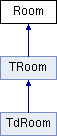
\includegraphics[height=3.000000cm]{class_room}
\end{center}
\end{figure}
\subsection*{Public Member Functions}
\begin{DoxyCompactItemize}
\item 
\hyperlink{class_room_a5fd7380ec44c3e7c4c85cde194c8c4c5}{Room} (string filename, string scriptname)
\begin{DoxyCompactList}\small\item\em D\-E\-P\-R\-E\-C\-A\-T\-E\-D\-: The constructor. \end{DoxyCompactList}\item 
\hyperlink{class_room_ac6ef93a7d9c3e1d624e025058d5f16ff}{Room} ()
\begin{DoxyCompactList}\small\item\em The simple constructor. \end{DoxyCompactList}\item 
\hyperlink{class_room_aec8c6468cfa356445e072430df3ed73b}{Room} (int w, int h)
\begin{DoxyCompactList}\small\item\em The intermediate constructor. \end{DoxyCompactList}\item 
\hyperlink{class_room_a67d5da09983cc53097807fd43ba5481a}{$\sim$\-Room} ()
\begin{DoxyCompactList}\small\item\em The destructor. \end{DoxyCompactList}\item 
void \hyperlink{class_room_ae996c7c2c5dcecd0e92b62d631978a89}{parse\-Objects} (map$<$ string, \hyperlink{class_object}{Object} $\ast$($\ast$)(float, float, \hyperlink{class_room}{Room} $\ast$)$>$ object\-Map)
\begin{DoxyCompactList}\small\item\em Creates all instances in the \hyperlink{class_room}{Room}. \end{DoxyCompactList}\item 
int \hyperlink{class_room_a297c938f6a2e911b6ae846e795d6d05e}{get\-Width} ()
\begin{DoxyCompactList}\small\item\em Get the \hyperlink{class_room}{Room}'s width. \end{DoxyCompactList}\item 
int \hyperlink{class_room_acbc864ff80ab5e2782a9bbcf78377e06}{get\-Height} ()
\begin{DoxyCompactList}\small\item\em Get the \hyperlink{class_room}{Room}'s height. \end{DoxyCompactList}\item 
void \hyperlink{class_room_aee02820d3a2a3c70d59e2f0455338cd7}{set\-Camera} (\hyperlink{class_camera}{Camera} $\ast$c)
\begin{DoxyCompactList}\small\item\em Sets the pointer to the default \hyperlink{class_camera}{Camera} instance. \end{DoxyCompactList}\item 
void \hyperlink{class_room_acf9689e04f8bc98d658d12d62b95e8bf}{add\-Object} (\hyperlink{class_object}{Object} $\ast$object)
\begin{DoxyCompactList}\small\item\em Adds an \hyperlink{class_object}{Object} to the \hyperlink{class_room}{Room}. \end{DoxyCompactList}\item 
void \hyperlink{class_room_ac9b5844f9e5e251d95ec60c3ec2bc1b6}{add\-Background} (\hyperlink{class_background}{Background} $\ast$background)
\begin{DoxyCompactList}\small\item\em Adds a \hyperlink{class_background}{Background} to the \hyperlink{class_room}{Room}. \end{DoxyCompactList}\item 
virtual void \hyperlink{class_room_a801c3de6ddff533edeb8fa68c7fcbb61}{update} ()
\begin{DoxyCompactList}\small\item\em The update method. \end{DoxyCompactList}\end{DoxyCompactItemize}
\subsection*{Public Attributes}
\begin{DoxyCompactItemize}
\item 
\hyperlink{class_camera}{Camera} $\ast$ \hyperlink{class_room_ae5dbd0283ba91cb66a53fd6f5229c4a3}{camera}
\begin{DoxyCompactList}\small\item\em The default camera. \end{DoxyCompactList}\item 
\hyperlink{class_room}{Room} $\ast$ \hyperlink{class_room_afc2baf90e55312f4a8b4967d0c7122db}{next\-Room}
\begin{DoxyCompactList}\small\item\em Next \hyperlink{class_room}{Room} pointer (when transitioning). \end{DoxyCompactList}\item 
\hyperlink{class_room}{Room} $\ast$ \hyperlink{class_room_a18aec7a7911d1d4874267f1d7dcaf1a6}{prev\-Room}
\begin{DoxyCompactList}\small\item\em Previous \hyperlink{class_room}{Room} pointer (in case you need it). \end{DoxyCompactList}\end{DoxyCompactItemize}
\subsection*{Protected Attributes}
\begin{DoxyCompactItemize}
\item 
xml\-\_\-node $\ast$ \hyperlink{class_room_a865810da64fc41a3a0858e4e7b5b5241}{map\-\_\-node}
\item 
int \hyperlink{class_room_a0c68c6762e7d93eb459ba552dadaf308}{width}
\item 
int \hyperlink{class_room_ab7d56b80d9eeefca79a2e83447ad4d66}{height}
\item 
int \hyperlink{class_room_ac2d78d3f1097249ae3a447ebe907ed9c}{wtile}
\item 
int \hyperlink{class_room_a2925415ce7fb199e496ad61b77e256cb}{htile}
\item 
int \hyperlink{class_room_aa5480a57c054045be3c677e43e358357}{wtileset}
\item 
int \hyperlink{class_room_ac6125cd56db3bf38d2f44158159b3899}{pfirstgid}
\item 
vector$<$ \hyperlink{class_object}{Object} $\ast$ $>$ \hyperlink{class_room_a6495b4a5cd0ea4979fcfbbb27c6b419e}{objects}
\item 
vector$<$ \hyperlink{class_background}{Background} $\ast$ $>$ \hyperlink{class_room_a2fc816969da445fc7f0bbb3ff7a5ca9f}{backgrounds}
\item 
vector$<$ event $>$ \hyperlink{class_room_a881d5a108a9a3aba5f44279ebbd8a4f9}{events}
\item 
vector$<$ vector$<$ vector$<$ int $>$ $>$ $>$ \hyperlink{class_room_aba520dbf1dd1907f5cdcbc8b6372ec53}{tmap}
\item 
vector$<$ vector$<$ int $>$ $>$ \hyperlink{class_room_a37b095fddfc6230033ed1de7afd9ec8d}{pmap}
\item 
S\-D\-L\-\_\-\-Texture $\ast$ \hyperlink{class_room_a5cd50f4bfda869d4ad45cb52c7e97f5b}{tileset}
\end{DoxyCompactItemize}
\subsection*{Friends}
\begin{DoxyCompactItemize}
\item 
class \hyperlink{class_room_ae5cfe0c0e0b06d536d5814bd1ff4818f}{Graphics}
\item 
class \hyperlink{class_room_a614439ccac0344926adc4c0165d64060}{Entity}
\item 
bool \hyperlink{class_room_ae842d44dccbe2dfeb3671612e0a3e377}{compare\-Objects\-By\-Depth} (\hyperlink{class_object}{Object} $\ast$obj1, \hyperlink{class_object}{Object} $\ast$obj2)
\begin{DoxyCompactList}\small\item\em A function that sorts Sprites by its depth. \end{DoxyCompactList}\item 
bool \hyperlink{class_room_aa580169e4f3c63e66b19f5216034eb54}{compare\-Backgrounds\-By\-Depth} (\hyperlink{class_background}{Background} $\ast$bg1, \hyperlink{class_background}{Background} $\ast$bg2)
\item 
void \hyperlink{class_room_aae5aa308717d7affd253c3645b9e011b}{S2\-M\-\_\-\-Room\-::\-Load\-Script} (string filename)
\item 
void \hyperlink{class_room_a85c37ccb227fe7bcf3252708caa40d56}{S2\-M\-\_\-\-Room\-::\-Load\-Script} ()
\end{DoxyCompactItemize}


\subsection{Detailed Description}
An abstraction of a certain space within a game. 

Rooms are a very abstract concept, much like objects. They represent a certain part of the game, like a level, the game menu or the rolling credits screen. 

\subsection{Constructor \& Destructor Documentation}
\hypertarget{class_room_a5fd7380ec44c3e7c4c85cde194c8c4c5}{\index{Room@{Room}!Room@{Room}}
\index{Room@{Room}!Room@{Room}}
\subsubsection[{Room}]{\setlength{\rightskip}{0pt plus 5cm}Room\-::\-Room (
\begin{DoxyParamCaption}
\item[{string}]{filename, }
\item[{string}]{scriptname}
\end{DoxyParamCaption}
)}}\label{class_room_a5fd7380ec44c3e7c4c85cde194c8c4c5}


D\-E\-P\-R\-E\-C\-A\-T\-E\-D\-: The constructor. 

Creates a \hyperlink{class_room}{Room} from a file. 
\begin{DoxyParams}{Parameters}
{\em filename} & the design file \\
\hline
{\em scriptname} & the script file \\
\hline
\end{DoxyParams}
\hypertarget{class_room_ac6ef93a7d9c3e1d624e025058d5f16ff}{\index{Room@{Room}!Room@{Room}}
\index{Room@{Room}!Room@{Room}}
\subsubsection[{Room}]{\setlength{\rightskip}{0pt plus 5cm}Room\-::\-Room (
\begin{DoxyParamCaption}
{}
\end{DoxyParamCaption}
)}}\label{class_room_ac6ef93a7d9c3e1d624e025058d5f16ff}


The simple constructor. 

Creates an empty black \hyperlink{class_room}{Room} with the game dimensions. \hypertarget{class_room_aec8c6468cfa356445e072430df3ed73b}{\index{Room@{Room}!Room@{Room}}
\index{Room@{Room}!Room@{Room}}
\subsubsection[{Room}]{\setlength{\rightskip}{0pt plus 5cm}Room\-::\-Room (
\begin{DoxyParamCaption}
\item[{int}]{w, }
\item[{int}]{h}
\end{DoxyParamCaption}
)}}\label{class_room_aec8c6468cfa356445e072430df3ed73b}


The intermediate constructor. 

Creates an empty black \hyperlink{class_room}{Room} with the specified dimensions. 
\begin{DoxyParams}{Parameters}
{\em w} & the \hyperlink{class_room}{Room}'s width \\
\hline
{\em h} & the Rooms height \\
\hline
\end{DoxyParams}
\hypertarget{class_room_a67d5da09983cc53097807fd43ba5481a}{\index{Room@{Room}!$\sim$\-Room@{$\sim$\-Room}}
\index{$\sim$\-Room@{$\sim$\-Room}!Room@{Room}}
\subsubsection[{$\sim$\-Room}]{\setlength{\rightskip}{0pt plus 5cm}Room\-::$\sim$\-Room (
\begin{DoxyParamCaption}
{}
\end{DoxyParamCaption}
)}}\label{class_room_a67d5da09983cc53097807fd43ba5481a}


The destructor. 

Destroys the \hyperlink{class_room}{Room} and all its associated tile textures. 

\subsection{Member Function Documentation}
\hypertarget{class_room_ac9b5844f9e5e251d95ec60c3ec2bc1b6}{\index{Room@{Room}!add\-Background@{add\-Background}}
\index{add\-Background@{add\-Background}!Room@{Room}}
\subsubsection[{add\-Background}]{\setlength{\rightskip}{0pt plus 5cm}void Room\-::add\-Background (
\begin{DoxyParamCaption}
\item[{{\bf Background} $\ast$}]{background}
\end{DoxyParamCaption}
)}}\label{class_room_ac9b5844f9e5e251d95ec60c3ec2bc1b6}


Adds a \hyperlink{class_background}{Background} to the \hyperlink{class_room}{Room}. 

Right after this the background vector will get sorted. 
\begin{DoxyParams}{Parameters}
{\em object} & the \hyperlink{class_background}{Background} to add. \\
\hline
\end{DoxyParams}
\begin{DoxySeeAlso}{See Also}
\hyperlink{class_room_acf9689e04f8bc98d658d12d62b95e8bf}{add\-Object()} 
\end{DoxySeeAlso}
\hypertarget{class_room_acf9689e04f8bc98d658d12d62b95e8bf}{\index{Room@{Room}!add\-Object@{add\-Object}}
\index{add\-Object@{add\-Object}!Room@{Room}}
\subsubsection[{add\-Object}]{\setlength{\rightskip}{0pt plus 5cm}void Room\-::add\-Object (
\begin{DoxyParamCaption}
\item[{{\bf Object} $\ast$}]{object}
\end{DoxyParamCaption}
)}}\label{class_room_acf9689e04f8bc98d658d12d62b95e8bf}


Adds an \hyperlink{class_object}{Object} to the \hyperlink{class_room}{Room}. 


\begin{DoxyParams}{Parameters}
{\em object} & the \hyperlink{class_object}{Object} to add. \\
\hline
\end{DoxyParams}
\begin{DoxySeeAlso}{See Also}
\hyperlink{class_room_ac9b5844f9e5e251d95ec60c3ec2bc1b6}{add\-Background()} 
\end{DoxySeeAlso}
\hypertarget{class_room_acbc864ff80ab5e2782a9bbcf78377e06}{\index{Room@{Room}!get\-Height@{get\-Height}}
\index{get\-Height@{get\-Height}!Room@{Room}}
\subsubsection[{get\-Height}]{\setlength{\rightskip}{0pt plus 5cm}int Room\-::get\-Height (
\begin{DoxyParamCaption}
{}
\end{DoxyParamCaption}
)}}\label{class_room_acbc864ff80ab5e2782a9bbcf78377e06}


Get the \hyperlink{class_room}{Room}'s height. 

\begin{DoxyReturn}{Returns}
the \hyperlink{class_room}{Room}'s height 
\end{DoxyReturn}
\begin{DoxySeeAlso}{See Also}
\hyperlink{class_room_a297c938f6a2e911b6ae846e795d6d05e}{get\-Width()} 
\end{DoxySeeAlso}
\hypertarget{class_room_a297c938f6a2e911b6ae846e795d6d05e}{\index{Room@{Room}!get\-Width@{get\-Width}}
\index{get\-Width@{get\-Width}!Room@{Room}}
\subsubsection[{get\-Width}]{\setlength{\rightskip}{0pt plus 5cm}int Room\-::get\-Width (
\begin{DoxyParamCaption}
{}
\end{DoxyParamCaption}
)}}\label{class_room_a297c938f6a2e911b6ae846e795d6d05e}


Get the \hyperlink{class_room}{Room}'s width. 

\begin{DoxyReturn}{Returns}
the \hyperlink{class_room}{Room}'s width 
\end{DoxyReturn}
\begin{DoxySeeAlso}{See Also}
\hyperlink{class_room_acbc864ff80ab5e2782a9bbcf78377e06}{get\-Height()} 
\end{DoxySeeAlso}
\hypertarget{class_room_ae996c7c2c5dcecd0e92b62d631978a89}{\index{Room@{Room}!parse\-Objects@{parse\-Objects}}
\index{parse\-Objects@{parse\-Objects}!Room@{Room}}
\subsubsection[{parse\-Objects}]{\setlength{\rightskip}{0pt plus 5cm}void Room\-::parse\-Objects (
\begin{DoxyParamCaption}
\item[{map$<$ string, {\bf Object} $\ast$($\ast$)(float, float, {\bf Room} $\ast$)$>$}]{object\-Map}
\end{DoxyParamCaption}
)}}\label{class_room_ae996c7c2c5dcecd0e92b62d631978a89}


Creates all instances in the \hyperlink{class_room}{Room}. 

\hypertarget{class_room_aee02820d3a2a3c70d59e2f0455338cd7}{\index{Room@{Room}!set\-Camera@{set\-Camera}}
\index{set\-Camera@{set\-Camera}!Room@{Room}}
\subsubsection[{set\-Camera}]{\setlength{\rightskip}{0pt plus 5cm}void Room\-::set\-Camera (
\begin{DoxyParamCaption}
\item[{{\bf Camera} $\ast$}]{c}
\end{DoxyParamCaption}
)}}\label{class_room_aee02820d3a2a3c70d59e2f0455338cd7}


Sets the pointer to the default \hyperlink{class_camera}{Camera} instance. 

The \hyperlink{class_graphics}{Graphics} instance needs a \hyperlink{class_camera}{Camera} instance pointer in order to know at any moment which part of the \hyperlink{class_room}{Room} to draw on the screen. 
\begin{DoxyParams}{Parameters}
{\em camera} & a pointer to a \hyperlink{class_camera}{Camera} instance \\
\hline
\end{DoxyParams}
\hypertarget{class_room_a801c3de6ddff533edeb8fa68c7fcbb61}{\index{Room@{Room}!update@{update}}
\index{update@{update}!Room@{Room}}
\subsubsection[{update}]{\setlength{\rightskip}{0pt plus 5cm}void Room\-::update (
\begin{DoxyParamCaption}
{}
\end{DoxyParamCaption}
)\hspace{0.3cm}{\ttfamily [virtual]}}}\label{class_room_a801c3de6ddff533edeb8fa68c7fcbb61}


The update method. 



\subsection{Friends And Related Function Documentation}
\hypertarget{class_room_aa580169e4f3c63e66b19f5216034eb54}{\index{Room@{Room}!compare\-Backgrounds\-By\-Depth@{compare\-Backgrounds\-By\-Depth}}
\index{compare\-Backgrounds\-By\-Depth@{compare\-Backgrounds\-By\-Depth}!Room@{Room}}
\subsubsection[{compare\-Backgrounds\-By\-Depth}]{\setlength{\rightskip}{0pt plus 5cm}bool compare\-Backgrounds\-By\-Depth (
\begin{DoxyParamCaption}
\item[{{\bf Background} $\ast$}]{bg1, }
\item[{{\bf Background} $\ast$}]{bg2}
\end{DoxyParamCaption}
)\hspace{0.3cm}{\ttfamily [friend]}}}\label{class_room_aa580169e4f3c63e66b19f5216034eb54}
\hypertarget{class_room_ae842d44dccbe2dfeb3671612e0a3e377}{\index{Room@{Room}!compare\-Objects\-By\-Depth@{compare\-Objects\-By\-Depth}}
\index{compare\-Objects\-By\-Depth@{compare\-Objects\-By\-Depth}!Room@{Room}}
\subsubsection[{compare\-Objects\-By\-Depth}]{\setlength{\rightskip}{0pt plus 5cm}bool compare\-Objects\-By\-Depth (
\begin{DoxyParamCaption}
\item[{{\bf Object} $\ast$}]{obj1, }
\item[{{\bf Object} $\ast$}]{obj2}
\end{DoxyParamCaption}
)\hspace{0.3cm}{\ttfamily [friend]}}}\label{class_room_ae842d44dccbe2dfeb3671612e0a3e377}


A function that sorts Sprites by its depth. 

\hypertarget{class_room_a614439ccac0344926adc4c0165d64060}{\index{Room@{Room}!Entity@{Entity}}
\index{Entity@{Entity}!Room@{Room}}
\subsubsection[{Entity}]{\setlength{\rightskip}{0pt plus 5cm}friend class {\bf Entity}\hspace{0.3cm}{\ttfamily [friend]}}}\label{class_room_a614439ccac0344926adc4c0165d64060}
\hypertarget{class_room_ae5cfe0c0e0b06d536d5814bd1ff4818f}{\index{Room@{Room}!Graphics@{Graphics}}
\index{Graphics@{Graphics}!Room@{Room}}
\subsubsection[{Graphics}]{\setlength{\rightskip}{0pt plus 5cm}friend class {\bf Graphics}\hspace{0.3cm}{\ttfamily [friend]}}}\label{class_room_ae5cfe0c0e0b06d536d5814bd1ff4818f}
\hypertarget{class_room_aae5aa308717d7affd253c3645b9e011b}{\index{Room@{Room}!S2\-M\-\_\-\-Room\-::\-Load\-Script@{S2\-M\-\_\-\-Room\-::\-Load\-Script}}
\index{S2\-M\-\_\-\-Room\-::\-Load\-Script@{S2\-M\-\_\-\-Room\-::\-Load\-Script}!Room@{Room}}
\subsubsection[{S2\-M\-\_\-\-Room\-::\-Load\-Script}]{\setlength{\rightskip}{0pt plus 5cm}void {\bf S2\-M\-\_\-\-Room\-::\-Load\-Script} (
\begin{DoxyParamCaption}
\item[{string}]{filename}
\end{DoxyParamCaption}
)\hspace{0.3cm}{\ttfamily [friend]}}}\label{class_room_aae5aa308717d7affd253c3645b9e011b}
\hypertarget{class_room_a85c37ccb227fe7bcf3252708caa40d56}{\index{Room@{Room}!S2\-M\-\_\-\-Room\-::\-Load\-Script@{S2\-M\-\_\-\-Room\-::\-Load\-Script}}
\index{S2\-M\-\_\-\-Room\-::\-Load\-Script@{S2\-M\-\_\-\-Room\-::\-Load\-Script}!Room@{Room}}
\subsubsection[{S2\-M\-\_\-\-Room\-::\-Load\-Script}]{\setlength{\rightskip}{0pt plus 5cm}void {\bf S2\-M\-\_\-\-Room\-::\-Load\-Script} (
\begin{DoxyParamCaption}
{}
\end{DoxyParamCaption}
)\hspace{0.3cm}{\ttfamily [friend]}}}\label{class_room_a85c37ccb227fe7bcf3252708caa40d56}


\subsection{Member Data Documentation}
\hypertarget{class_room_a2fc816969da445fc7f0bbb3ff7a5ca9f}{\index{Room@{Room}!backgrounds@{backgrounds}}
\index{backgrounds@{backgrounds}!Room@{Room}}
\subsubsection[{backgrounds}]{\setlength{\rightskip}{0pt plus 5cm}vector$<${\bf Background} $\ast$$>$ Room\-::backgrounds\hspace{0.3cm}{\ttfamily [protected]}}}\label{class_room_a2fc816969da445fc7f0bbb3ff7a5ca9f}
\hypertarget{class_room_ae5dbd0283ba91cb66a53fd6f5229c4a3}{\index{Room@{Room}!camera@{camera}}
\index{camera@{camera}!Room@{Room}}
\subsubsection[{camera}]{\setlength{\rightskip}{0pt plus 5cm}{\bf Camera}$\ast$ Room\-::camera}}\label{class_room_ae5dbd0283ba91cb66a53fd6f5229c4a3}


The default camera. 

\hypertarget{class_room_a881d5a108a9a3aba5f44279ebbd8a4f9}{\index{Room@{Room}!events@{events}}
\index{events@{events}!Room@{Room}}
\subsubsection[{events}]{\setlength{\rightskip}{0pt plus 5cm}vector$<$event$>$ Room\-::events\hspace{0.3cm}{\ttfamily [protected]}}}\label{class_room_a881d5a108a9a3aba5f44279ebbd8a4f9}
\hypertarget{class_room_ab7d56b80d9eeefca79a2e83447ad4d66}{\index{Room@{Room}!height@{height}}
\index{height@{height}!Room@{Room}}
\subsubsection[{height}]{\setlength{\rightskip}{0pt plus 5cm}int Room\-::height\hspace{0.3cm}{\ttfamily [protected]}}}\label{class_room_ab7d56b80d9eeefca79a2e83447ad4d66}
\hypertarget{class_room_a2925415ce7fb199e496ad61b77e256cb}{\index{Room@{Room}!htile@{htile}}
\index{htile@{htile}!Room@{Room}}
\subsubsection[{htile}]{\setlength{\rightskip}{0pt plus 5cm}int Room\-::htile\hspace{0.3cm}{\ttfamily [protected]}}}\label{class_room_a2925415ce7fb199e496ad61b77e256cb}
\hypertarget{class_room_a865810da64fc41a3a0858e4e7b5b5241}{\index{Room@{Room}!map\-\_\-node@{map\-\_\-node}}
\index{map\-\_\-node@{map\-\_\-node}!Room@{Room}}
\subsubsection[{map\-\_\-node}]{\setlength{\rightskip}{0pt plus 5cm}xml\-\_\-node$\ast$ Room\-::map\-\_\-node\hspace{0.3cm}{\ttfamily [protected]}}}\label{class_room_a865810da64fc41a3a0858e4e7b5b5241}
\hypertarget{class_room_afc2baf90e55312f4a8b4967d0c7122db}{\index{Room@{Room}!next\-Room@{next\-Room}}
\index{next\-Room@{next\-Room}!Room@{Room}}
\subsubsection[{next\-Room}]{\setlength{\rightskip}{0pt plus 5cm}{\bf Room}$\ast$ Room\-::next\-Room}}\label{class_room_afc2baf90e55312f4a8b4967d0c7122db}


Next \hyperlink{class_room}{Room} pointer (when transitioning). 

\hypertarget{class_room_a6495b4a5cd0ea4979fcfbbb27c6b419e}{\index{Room@{Room}!objects@{objects}}
\index{objects@{objects}!Room@{Room}}
\subsubsection[{objects}]{\setlength{\rightskip}{0pt plus 5cm}vector$<${\bf Object} $\ast$$>$ Room\-::objects\hspace{0.3cm}{\ttfamily [protected]}}}\label{class_room_a6495b4a5cd0ea4979fcfbbb27c6b419e}
\hypertarget{class_room_ac6125cd56db3bf38d2f44158159b3899}{\index{Room@{Room}!pfirstgid@{pfirstgid}}
\index{pfirstgid@{pfirstgid}!Room@{Room}}
\subsubsection[{pfirstgid}]{\setlength{\rightskip}{0pt plus 5cm}int Room\-::pfirstgid\hspace{0.3cm}{\ttfamily [protected]}}}\label{class_room_ac6125cd56db3bf38d2f44158159b3899}
\hypertarget{class_room_a37b095fddfc6230033ed1de7afd9ec8d}{\index{Room@{Room}!pmap@{pmap}}
\index{pmap@{pmap}!Room@{Room}}
\subsubsection[{pmap}]{\setlength{\rightskip}{0pt plus 5cm}vector$<$vector$<$int$>$ $>$ Room\-::pmap\hspace{0.3cm}{\ttfamily [protected]}}}\label{class_room_a37b095fddfc6230033ed1de7afd9ec8d}
\hypertarget{class_room_a18aec7a7911d1d4874267f1d7dcaf1a6}{\index{Room@{Room}!prev\-Room@{prev\-Room}}
\index{prev\-Room@{prev\-Room}!Room@{Room}}
\subsubsection[{prev\-Room}]{\setlength{\rightskip}{0pt plus 5cm}{\bf Room}$\ast$ Room\-::prev\-Room}}\label{class_room_a18aec7a7911d1d4874267f1d7dcaf1a6}


Previous \hyperlink{class_room}{Room} pointer (in case you need it). 

\hypertarget{class_room_a5cd50f4bfda869d4ad45cb52c7e97f5b}{\index{Room@{Room}!tileset@{tileset}}
\index{tileset@{tileset}!Room@{Room}}
\subsubsection[{tileset}]{\setlength{\rightskip}{0pt plus 5cm}S\-D\-L\-\_\-\-Texture$\ast$ Room\-::tileset\hspace{0.3cm}{\ttfamily [protected]}}}\label{class_room_a5cd50f4bfda869d4ad45cb52c7e97f5b}
\hypertarget{class_room_aba520dbf1dd1907f5cdcbc8b6372ec53}{\index{Room@{Room}!tmap@{tmap}}
\index{tmap@{tmap}!Room@{Room}}
\subsubsection[{tmap}]{\setlength{\rightskip}{0pt plus 5cm}vector$<$vector$<$vector$<$int$>$ $>$ $>$ Room\-::tmap\hspace{0.3cm}{\ttfamily [protected]}}}\label{class_room_aba520dbf1dd1907f5cdcbc8b6372ec53}
\hypertarget{class_room_a0c68c6762e7d93eb459ba552dadaf308}{\index{Room@{Room}!width@{width}}
\index{width@{width}!Room@{Room}}
\subsubsection[{width}]{\setlength{\rightskip}{0pt plus 5cm}int Room\-::width\hspace{0.3cm}{\ttfamily [protected]}}}\label{class_room_a0c68c6762e7d93eb459ba552dadaf308}
\hypertarget{class_room_ac2d78d3f1097249ae3a447ebe907ed9c}{\index{Room@{Room}!wtile@{wtile}}
\index{wtile@{wtile}!Room@{Room}}
\subsubsection[{wtile}]{\setlength{\rightskip}{0pt plus 5cm}int Room\-::wtile\hspace{0.3cm}{\ttfamily [protected]}}}\label{class_room_ac2d78d3f1097249ae3a447ebe907ed9c}
\hypertarget{class_room_aa5480a57c054045be3c677e43e358357}{\index{Room@{Room}!wtileset@{wtileset}}
\index{wtileset@{wtileset}!Room@{Room}}
\subsubsection[{wtileset}]{\setlength{\rightskip}{0pt plus 5cm}int Room\-::wtileset\hspace{0.3cm}{\ttfamily [protected]}}}\label{class_room_aa5480a57c054045be3c677e43e358357}


The documentation for this class was generated from the following files\-:\begin{DoxyCompactItemize}
\item 
src/\hyperlink{room_8h}{room.\-h}\item 
src/\hyperlink{room_8cpp}{room.\-cpp}\end{DoxyCompactItemize}

\input{class_sound}
\hypertarget{class_sprite}{\section{Sprite Class Reference}
\label{class_sprite}\index{Sprite@{Sprite}}
}


A simple abstraction of a set of images and animations.  




{\ttfamily \#include $<$graphics.\-h$>$}

\subsection*{Public Member Functions}
\begin{DoxyCompactItemize}
\item 
\hyperlink{class_sprite_ae389173729bb257ec701c29830e55c38}{Sprite} (string filename, int w, int h)
\begin{DoxyCompactList}\small\item\em The constructor. \end{DoxyCompactList}\item 
\hyperlink{class_sprite_a8accab430f9d90ae5117b57d67e32b84}{$\sim$\-Sprite} ()
\begin{DoxyCompactList}\small\item\em The destructor. \end{DoxyCompactList}\item 
int \hyperlink{class_sprite_aba3d4752461ec679fbf5de7ec4c34f61}{get\-Width} ()
\begin{DoxyCompactList}\small\item\em Returns the \hyperlink{class_sprite}{Sprite}'s width. \end{DoxyCompactList}\item 
int \hyperlink{class_sprite_a67b67082cfda90103d2d9eefea04cc4b}{get\-Height} ()
\begin{DoxyCompactList}\small\item\em Returns the \hyperlink{class_sprite}{Sprite}'s height. \end{DoxyCompactList}\item 
void \hyperlink{class_sprite_ae717a7440c08698741f7642a0ea2c28b}{set\-Center} (int xc, int yc)
\begin{DoxyCompactList}\small\item\em Sets both the horizontal and vertical coordinates of the \hyperlink{class_sprite}{Sprite}'s center. \end{DoxyCompactList}\item 
int \hyperlink{class_sprite_a2863e4b0262fc2039a9dec95659fafc2}{get\-X\-Center} ()
\item 
int \hyperlink{class_sprite_ab7f9b251c7f95b8bbf7fc7d04038d477}{get\-Y\-Center} ()
\item 
S\-D\-L\-\_\-\-Rect $\ast$ \hyperlink{class_sprite_a8da8cdca88b50b2cf61bc9cd43a6c986}{get\-Rect} (int i)
\begin{DoxyCompactList}\small\item\em Gets the given frame's S\-D\-L\-\_\-\-Rect on the \hyperlink{class_sprite}{Sprite} texture. \end{DoxyCompactList}\item 
void \hyperlink{class_sprite_a7b6f244a3fcaa271d16b9c690c486c77}{add\-Animation} (vector$<$ int $>$ animation)
\begin{DoxyCompactList}\small\item\em Adds an animation to the animations vector. \end{DoxyCompactList}\item 
vector$<$ int $>$ \hyperlink{class_sprite_a6c29474804466ae43d379ec17885044a}{ret\-Animation} (int i)
\begin{DoxyCompactList}\small\item\em Gets an animation from the animations vector. \end{DoxyCompactList}\item 
int \hyperlink{class_sprite_a6f3e4a0efcff7c0ee234655c8a0ae80e}{get\-Animations\-Size} ()
\begin{DoxyCompactList}\small\item\em Get the total number of animations. \end{DoxyCompactList}\item 
virtual void \hyperlink{class_sprite_a6d0f7e628b4ea8540697605fff906759}{update} ()
\begin{DoxyCompactList}\small\item\em An overridable update method in case you need it (?). \end{DoxyCompactList}\end{DoxyCompactItemize}
\subsection*{Protected Attributes}
\begin{DoxyCompactItemize}
\item 
S\-D\-L\-\_\-\-Texture $\ast$ \hyperlink{class_sprite_a531ed274733d916261f49e1a2cbb6ba9}{texture}
\begin{DoxyCompactList}\small\item\em The texture containing every single frame of the \hyperlink{class_sprite}{Sprite}. \end{DoxyCompactList}\item 
int \hyperlink{class_sprite_a0a3364944c5e361fc9e7ae406224d682}{width}
\begin{DoxyCompactList}\small\item\em \hyperlink{class_sprite}{Sprite}'s width. \end{DoxyCompactList}\item 
int \hyperlink{class_sprite_a1f07c8f2080c193759aec0e13503d7ab}{height}
\begin{DoxyCompactList}\small\item\em \hyperlink{class_sprite}{Sprite}'s height. \end{DoxyCompactList}\item 
int \hyperlink{class_sprite_a342df27bc7e10f79c0bc4d89689e5bfe}{wtexture}
\begin{DoxyCompactList}\small\item\em \hyperlink{class_sprite}{Sprite}'s texture width. \end{DoxyCompactList}\item 
int \hyperlink{class_sprite_afa90435f9d50265180a80399fda091d1}{htexture}
\begin{DoxyCompactList}\small\item\em \hyperlink{class_sprite}{Sprite}'s texture height. \end{DoxyCompactList}\item 
int \hyperlink{class_sprite_a4fc7935f0e4e38f0960a412293c87ab2}{xcenter} = 0
\begin{DoxyCompactList}\small\item\em Horizontal coordinate of the \hyperlink{class_sprite}{Sprite}'s center. \end{DoxyCompactList}\item 
int \hyperlink{class_sprite_a5b63544c1057e1d90ccb4fb573e6db27}{ycenter} = 0
\begin{DoxyCompactList}\small\item\em Vertical coordinate of the \hyperlink{class_sprite}{Sprite}'s center. \end{DoxyCompactList}\item 
vector$<$ vector$<$ int $>$ $>$ \hyperlink{class_sprite_a53b4aa1ae4e205df76c5145934fd7c8f}{animations}
\begin{DoxyCompactList}\small\item\em Animation vector. \end{DoxyCompactList}\item 
vector$<$ vector$<$ S\-D\-L\-\_\-\-Rect $>$ $>$ \hyperlink{class_sprite_ad18e21f70d9bc3d1e52d2d4c25645e15}{bboxes}
\begin{DoxyCompactList}\small\item\em Vector containing each frame's bounding boxes. \end{DoxyCompactList}\item 
S\-D\-L\-\_\-\-Rect \hyperlink{class_sprite_ab8ae1fcc8b8fb328583438cf1f0b6e2f}{rect}
\begin{DoxyCompactList}\small\item\em Bounding Box. \end{DoxyCompactList}\end{DoxyCompactItemize}
\subsection*{Friends}
\begin{DoxyCompactItemize}
\item 
class \hyperlink{class_sprite_ae5cfe0c0e0b06d536d5814bd1ff4818f}{Graphics}
\item 
class \hyperlink{class_sprite_a0720b5f434e636e22a3ed34f847eec57}{Object}
\item 
void \hyperlink{class_sprite_af4cff1e3ae7e299888e9790c6252dc10}{Graphics\-::update} ()
\item 
void \hyperlink{class_sprite_a9338a05480ae44ecf5fa4f5fcf713bbb}{Object\-::update} ()
\end{DoxyCompactItemize}


\subsection{Detailed Description}
A simple abstraction of a set of images and animations. 

A \hyperlink{class_sprite}{Sprite} instance must be instantiated by each object who wants to have a screen representation. 

\subsection{Constructor \& Destructor Documentation}
\hypertarget{class_sprite_ae389173729bb257ec701c29830e55c38}{\index{Sprite@{Sprite}!Sprite@{Sprite}}
\index{Sprite@{Sprite}!Sprite@{Sprite}}
\subsubsection[{Sprite}]{\setlength{\rightskip}{0pt plus 5cm}Sprite\-::\-Sprite (
\begin{DoxyParamCaption}
\item[{string}]{filename, }
\item[{int}]{w, }
\item[{int}]{h}
\end{DoxyParamCaption}
)}}\label{class_sprite_ae389173729bb257ec701c29830e55c38}


The constructor. 


\begin{DoxyParams}{Parameters}
{\em filename} & the bitmap filename where all the sprite images are to be loaded \\
\hline
{\em w} & the width of each image \\
\hline
{\em h} & the height of each image \\
\hline
\end{DoxyParams}
\hypertarget{class_sprite_a8accab430f9d90ae5117b57d67e32b84}{\index{Sprite@{Sprite}!$\sim$\-Sprite@{$\sim$\-Sprite}}
\index{$\sim$\-Sprite@{$\sim$\-Sprite}!Sprite@{Sprite}}
\subsubsection[{$\sim$\-Sprite}]{\setlength{\rightskip}{0pt plus 5cm}Sprite\-::$\sim$\-Sprite (
\begin{DoxyParamCaption}
{}
\end{DoxyParamCaption}
)}}\label{class_sprite_a8accab430f9d90ae5117b57d67e32b84}


The destructor. 

Destroys the \hyperlink{class_sprite}{Sprite} and frees its textures. 

\subsection{Member Function Documentation}
\hypertarget{class_sprite_a7b6f244a3fcaa271d16b9c690c486c77}{\index{Sprite@{Sprite}!add\-Animation@{add\-Animation}}
\index{add\-Animation@{add\-Animation}!Sprite@{Sprite}}
\subsubsection[{add\-Animation}]{\setlength{\rightskip}{0pt plus 5cm}void Sprite\-::add\-Animation (
\begin{DoxyParamCaption}
\item[{vector$<$ int $>$}]{animation}
\end{DoxyParamCaption}
)}}\label{class_sprite_a7b6f244a3fcaa271d16b9c690c486c77}


Adds an animation to the animations vector. 

Each \hyperlink{class_sprite}{Sprite} has a vector of animations, which are nothing more than image numbers arranged by order. They play in sequence and in the established order. 
\begin{DoxyParams}{Parameters}
{\em animation} & a vector of numbers that represent frames \\
\hline
\end{DoxyParams}
\hypertarget{class_sprite_a6f3e4a0efcff7c0ee234655c8a0ae80e}{\index{Sprite@{Sprite}!get\-Animations\-Size@{get\-Animations\-Size}}
\index{get\-Animations\-Size@{get\-Animations\-Size}!Sprite@{Sprite}}
\subsubsection[{get\-Animations\-Size}]{\setlength{\rightskip}{0pt plus 5cm}int Sprite\-::get\-Animations\-Size (
\begin{DoxyParamCaption}
{}
\end{DoxyParamCaption}
)}}\label{class_sprite_a6f3e4a0efcff7c0ee234655c8a0ae80e}


Get the total number of animations. 

\begin{DoxyReturn}{Returns}
The total number of animations. 
\end{DoxyReturn}
\hypertarget{class_sprite_a67b67082cfda90103d2d9eefea04cc4b}{\index{Sprite@{Sprite}!get\-Height@{get\-Height}}
\index{get\-Height@{get\-Height}!Sprite@{Sprite}}
\subsubsection[{get\-Height}]{\setlength{\rightskip}{0pt plus 5cm}int Sprite\-::get\-Height (
\begin{DoxyParamCaption}
{}
\end{DoxyParamCaption}
)}}\label{class_sprite_a67b67082cfda90103d2d9eefea04cc4b}


Returns the \hyperlink{class_sprite}{Sprite}'s height. 

/return The \hyperlink{class_sprite}{Sprite}'s height. \hypertarget{class_sprite_a8da8cdca88b50b2cf61bc9cd43a6c986}{\index{Sprite@{Sprite}!get\-Rect@{get\-Rect}}
\index{get\-Rect@{get\-Rect}!Sprite@{Sprite}}
\subsubsection[{get\-Rect}]{\setlength{\rightskip}{0pt plus 5cm}S\-D\-L\-\_\-\-Rect $\ast$ Sprite\-::get\-Rect (
\begin{DoxyParamCaption}
\item[{int}]{i}
\end{DoxyParamCaption}
)}}\label{class_sprite_a8da8cdca88b50b2cf61bc9cd43a6c986}


Gets the given frame's S\-D\-L\-\_\-\-Rect on the \hyperlink{class_sprite}{Sprite} texture. 


\begin{DoxyParams}{Parameters}
{\em i} & the frame number \\
\hline
\end{DoxyParams}
\begin{DoxyReturn}{Returns}
A pointer to an S\-D\-L\-\_\-\-Rect structure. 
\end{DoxyReturn}
\hypertarget{class_sprite_aba3d4752461ec679fbf5de7ec4c34f61}{\index{Sprite@{Sprite}!get\-Width@{get\-Width}}
\index{get\-Width@{get\-Width}!Sprite@{Sprite}}
\subsubsection[{get\-Width}]{\setlength{\rightskip}{0pt plus 5cm}int Sprite\-::get\-Width (
\begin{DoxyParamCaption}
{}
\end{DoxyParamCaption}
)}}\label{class_sprite_aba3d4752461ec679fbf5de7ec4c34f61}


Returns the \hyperlink{class_sprite}{Sprite}'s width. 

/return The \hyperlink{class_sprite}{Sprite}'s width. \hypertarget{class_sprite_a2863e4b0262fc2039a9dec95659fafc2}{\index{Sprite@{Sprite}!get\-X\-Center@{get\-X\-Center}}
\index{get\-X\-Center@{get\-X\-Center}!Sprite@{Sprite}}
\subsubsection[{get\-X\-Center}]{\setlength{\rightskip}{0pt plus 5cm}int Sprite\-::get\-X\-Center (
\begin{DoxyParamCaption}
{}
\end{DoxyParamCaption}
)}}\label{class_sprite_a2863e4b0262fc2039a9dec95659fafc2}
\hypertarget{class_sprite_ab7f9b251c7f95b8bbf7fc7d04038d477}{\index{Sprite@{Sprite}!get\-Y\-Center@{get\-Y\-Center}}
\index{get\-Y\-Center@{get\-Y\-Center}!Sprite@{Sprite}}
\subsubsection[{get\-Y\-Center}]{\setlength{\rightskip}{0pt plus 5cm}int Sprite\-::get\-Y\-Center (
\begin{DoxyParamCaption}
{}
\end{DoxyParamCaption}
)}}\label{class_sprite_ab7f9b251c7f95b8bbf7fc7d04038d477}
\hypertarget{class_sprite_a6c29474804466ae43d379ec17885044a}{\index{Sprite@{Sprite}!ret\-Animation@{ret\-Animation}}
\index{ret\-Animation@{ret\-Animation}!Sprite@{Sprite}}
\subsubsection[{ret\-Animation}]{\setlength{\rightskip}{0pt plus 5cm}vector$<$ int $>$ Sprite\-::ret\-Animation (
\begin{DoxyParamCaption}
\item[{int}]{i}
\end{DoxyParamCaption}
)}}\label{class_sprite_a6c29474804466ae43d379ec17885044a}


Gets an animation from the animations vector. 


\begin{DoxyParams}{Parameters}
{\em i} & the animation index \\
\hline
\end{DoxyParams}
\begin{DoxyReturn}{Returns}
A vector containing the animation on the given index 
\end{DoxyReturn}
\hypertarget{class_sprite_ae717a7440c08698741f7642a0ea2c28b}{\index{Sprite@{Sprite}!set\-Center@{set\-Center}}
\index{set\-Center@{set\-Center}!Sprite@{Sprite}}
\subsubsection[{set\-Center}]{\setlength{\rightskip}{0pt plus 5cm}void Sprite\-::set\-Center (
\begin{DoxyParamCaption}
\item[{int}]{xc, }
\item[{int}]{yc}
\end{DoxyParamCaption}
)}}\label{class_sprite_ae717a7440c08698741f7642a0ea2c28b}


Sets both the horizontal and vertical coordinates of the \hyperlink{class_sprite}{Sprite}'s center. 


\begin{DoxyParams}{Parameters}
{\em x} & horizontal coordinate of the \hyperlink{class_sprite}{Sprite}'s center \\
\hline
{\em y} & vertical coordinate of the \hyperlink{class_sprite}{Sprite}'s center \\
\hline
\end{DoxyParams}
\hypertarget{class_sprite_a6d0f7e628b4ea8540697605fff906759}{\index{Sprite@{Sprite}!update@{update}}
\index{update@{update}!Sprite@{Sprite}}
\subsubsection[{update}]{\setlength{\rightskip}{0pt plus 5cm}void Sprite\-::update (
\begin{DoxyParamCaption}
{}
\end{DoxyParamCaption}
)\hspace{0.3cm}{\ttfamily [virtual]}}}\label{class_sprite_a6d0f7e628b4ea8540697605fff906759}


An overridable update method in case you need it (?). 



\subsection{Friends And Related Function Documentation}
\hypertarget{class_sprite_ae5cfe0c0e0b06d536d5814bd1ff4818f}{\index{Sprite@{Sprite}!Graphics@{Graphics}}
\index{Graphics@{Graphics}!Sprite@{Sprite}}
\subsubsection[{Graphics}]{\setlength{\rightskip}{0pt plus 5cm}friend class {\bf Graphics}\hspace{0.3cm}{\ttfamily [friend]}}}\label{class_sprite_ae5cfe0c0e0b06d536d5814bd1ff4818f}
\hypertarget{class_sprite_af4cff1e3ae7e299888e9790c6252dc10}{\index{Sprite@{Sprite}!Graphics\-::update@{Graphics\-::update}}
\index{Graphics\-::update@{Graphics\-::update}!Sprite@{Sprite}}
\subsubsection[{Graphics\-::update}]{\setlength{\rightskip}{0pt plus 5cm}void {\bf Graphics\-::update} (
\begin{DoxyParamCaption}
{}
\end{DoxyParamCaption}
)\hspace{0.3cm}{\ttfamily [friend]}}}\label{class_sprite_af4cff1e3ae7e299888e9790c6252dc10}
\hypertarget{class_sprite_a0720b5f434e636e22a3ed34f847eec57}{\index{Sprite@{Sprite}!Object@{Object}}
\index{Object@{Object}!Sprite@{Sprite}}
\subsubsection[{Object}]{\setlength{\rightskip}{0pt plus 5cm}friend class {\bf Object}\hspace{0.3cm}{\ttfamily [friend]}}}\label{class_sprite_a0720b5f434e636e22a3ed34f847eec57}
\hypertarget{class_sprite_a9338a05480ae44ecf5fa4f5fcf713bbb}{\index{Sprite@{Sprite}!Object\-::update@{Object\-::update}}
\index{Object\-::update@{Object\-::update}!Sprite@{Sprite}}
\subsubsection[{Object\-::update}]{\setlength{\rightskip}{0pt plus 5cm}void {\bf Object\-::update} (
\begin{DoxyParamCaption}
{}
\end{DoxyParamCaption}
)\hspace{0.3cm}{\ttfamily [friend]}}}\label{class_sprite_a9338a05480ae44ecf5fa4f5fcf713bbb}


\subsection{Member Data Documentation}
\hypertarget{class_sprite_a53b4aa1ae4e205df76c5145934fd7c8f}{\index{Sprite@{Sprite}!animations@{animations}}
\index{animations@{animations}!Sprite@{Sprite}}
\subsubsection[{animations}]{\setlength{\rightskip}{0pt plus 5cm}vector$<$ vector$<$int$>$ $>$ Sprite\-::animations\hspace{0.3cm}{\ttfamily [protected]}}}\label{class_sprite_a53b4aa1ae4e205df76c5145934fd7c8f}


Animation vector. 

\hypertarget{class_sprite_ad18e21f70d9bc3d1e52d2d4c25645e15}{\index{Sprite@{Sprite}!bboxes@{bboxes}}
\index{bboxes@{bboxes}!Sprite@{Sprite}}
\subsubsection[{bboxes}]{\setlength{\rightskip}{0pt plus 5cm}vector$<$ vector$<$S\-D\-L\-\_\-\-Rect$>$ $>$ Sprite\-::bboxes\hspace{0.3cm}{\ttfamily [protected]}}}\label{class_sprite_ad18e21f70d9bc3d1e52d2d4c25645e15}


Vector containing each frame's bounding boxes. 

\hypertarget{class_sprite_a1f07c8f2080c193759aec0e13503d7ab}{\index{Sprite@{Sprite}!height@{height}}
\index{height@{height}!Sprite@{Sprite}}
\subsubsection[{height}]{\setlength{\rightskip}{0pt plus 5cm}int Sprite\-::height\hspace{0.3cm}{\ttfamily [protected]}}}\label{class_sprite_a1f07c8f2080c193759aec0e13503d7ab}


\hyperlink{class_sprite}{Sprite}'s height. 

\hypertarget{class_sprite_afa90435f9d50265180a80399fda091d1}{\index{Sprite@{Sprite}!htexture@{htexture}}
\index{htexture@{htexture}!Sprite@{Sprite}}
\subsubsection[{htexture}]{\setlength{\rightskip}{0pt plus 5cm}int Sprite\-::htexture\hspace{0.3cm}{\ttfamily [protected]}}}\label{class_sprite_afa90435f9d50265180a80399fda091d1}


\hyperlink{class_sprite}{Sprite}'s texture height. 

\hypertarget{class_sprite_ab8ae1fcc8b8fb328583438cf1f0b6e2f}{\index{Sprite@{Sprite}!rect@{rect}}
\index{rect@{rect}!Sprite@{Sprite}}
\subsubsection[{rect}]{\setlength{\rightskip}{0pt plus 5cm}S\-D\-L\-\_\-\-Rect Sprite\-::rect\hspace{0.3cm}{\ttfamily [protected]}}}\label{class_sprite_ab8ae1fcc8b8fb328583438cf1f0b6e2f}


Bounding Box. 

\hypertarget{class_sprite_a531ed274733d916261f49e1a2cbb6ba9}{\index{Sprite@{Sprite}!texture@{texture}}
\index{texture@{texture}!Sprite@{Sprite}}
\subsubsection[{texture}]{\setlength{\rightskip}{0pt plus 5cm}S\-D\-L\-\_\-\-Texture$\ast$ Sprite\-::texture\hspace{0.3cm}{\ttfamily [protected]}}}\label{class_sprite_a531ed274733d916261f49e1a2cbb6ba9}


The texture containing every single frame of the \hyperlink{class_sprite}{Sprite}. 

\hypertarget{class_sprite_a0a3364944c5e361fc9e7ae406224d682}{\index{Sprite@{Sprite}!width@{width}}
\index{width@{width}!Sprite@{Sprite}}
\subsubsection[{width}]{\setlength{\rightskip}{0pt plus 5cm}int Sprite\-::width\hspace{0.3cm}{\ttfamily [protected]}}}\label{class_sprite_a0a3364944c5e361fc9e7ae406224d682}


\hyperlink{class_sprite}{Sprite}'s width. 

\hypertarget{class_sprite_a342df27bc7e10f79c0bc4d89689e5bfe}{\index{Sprite@{Sprite}!wtexture@{wtexture}}
\index{wtexture@{wtexture}!Sprite@{Sprite}}
\subsubsection[{wtexture}]{\setlength{\rightskip}{0pt plus 5cm}int Sprite\-::wtexture\hspace{0.3cm}{\ttfamily [protected]}}}\label{class_sprite_a342df27bc7e10f79c0bc4d89689e5bfe}


\hyperlink{class_sprite}{Sprite}'s texture width. 

\hypertarget{class_sprite_a4fc7935f0e4e38f0960a412293c87ab2}{\index{Sprite@{Sprite}!xcenter@{xcenter}}
\index{xcenter@{xcenter}!Sprite@{Sprite}}
\subsubsection[{xcenter}]{\setlength{\rightskip}{0pt plus 5cm}int Sprite\-::xcenter = 0\hspace{0.3cm}{\ttfamily [protected]}}}\label{class_sprite_a4fc7935f0e4e38f0960a412293c87ab2}


Horizontal coordinate of the \hyperlink{class_sprite}{Sprite}'s center. 

\hypertarget{class_sprite_a5b63544c1057e1d90ccb4fb573e6db27}{\index{Sprite@{Sprite}!ycenter@{ycenter}}
\index{ycenter@{ycenter}!Sprite@{Sprite}}
\subsubsection[{ycenter}]{\setlength{\rightskip}{0pt plus 5cm}int Sprite\-::ycenter = 0\hspace{0.3cm}{\ttfamily [protected]}}}\label{class_sprite_a5b63544c1057e1d90ccb4fb573e6db27}


Vertical coordinate of the \hyperlink{class_sprite}{Sprite}'s center. 



The documentation for this class was generated from the following files\-:\begin{DoxyCompactItemize}
\item 
src/\hyperlink{graphics_8h}{graphics.\-h}\item 
src/\hyperlink{graphics_8cpp}{graphics.\-cpp}\end{DoxyCompactItemize}

\input{class_td_room}
\input{class_transition}
\input{class_t_room}
\hypertarget{class_virtual_joystick}{\section{Virtual\-Joystick Class Reference}
\label{class_virtual_joystick}\index{Virtual\-Joystick@{Virtual\-Joystick}}
}


Virtual representation of game buttons/keys.  




{\ttfamily \#include $<$joystick.\-h$>$}

Inheritance diagram for Virtual\-Joystick\-:\begin{figure}[H]
\begin{center}
\leavevmode
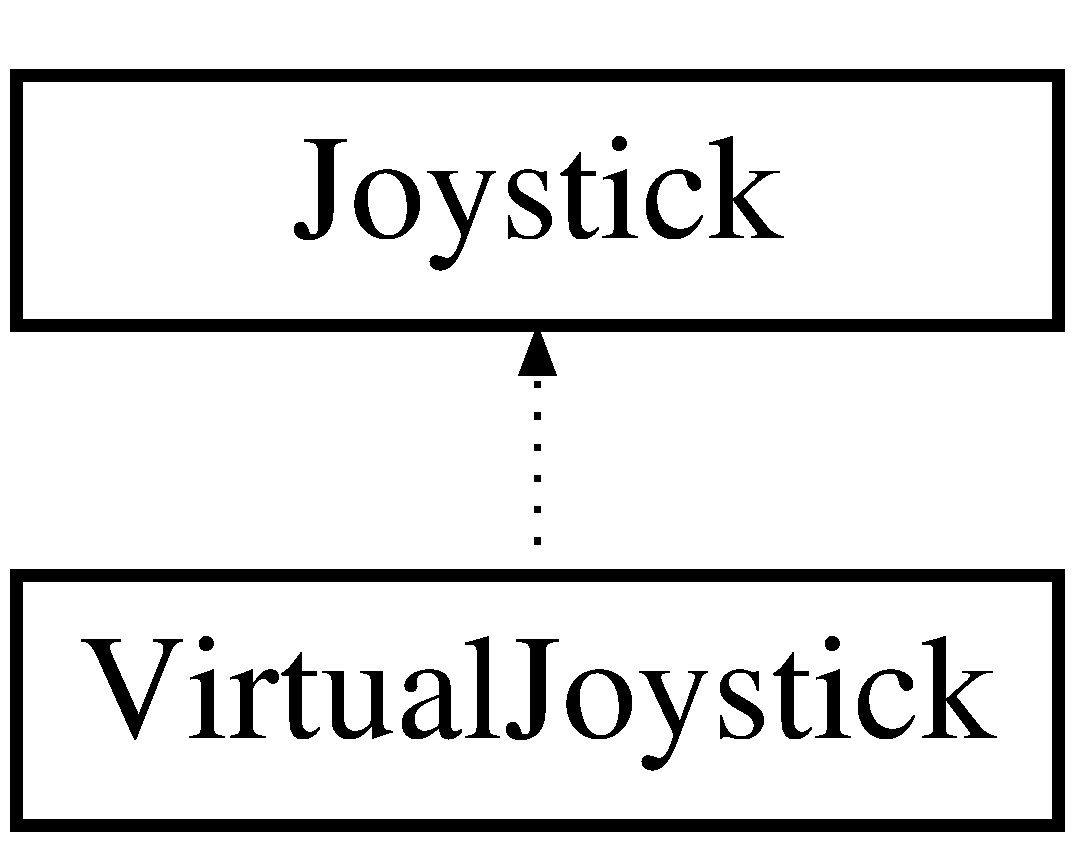
\includegraphics[height=2.000000cm]{class_virtual_joystick}
\end{center}
\end{figure}


\subsection{Detailed Description}
Virtual representation of game buttons/keys. 

Careful, because this may be confusing\-: A \hyperlink{class_virtual_joystick}{Virtual\-Joystick} is a virtual representation of the game buttons. It is useful whenever we want to make an \hyperlink{class_entity}{Entity} move, because assigning a \hyperlink{class_joystick}{Joystick} to it (if it doesn't already have one, which is probable since it is created by the constructor) we can code the \hyperlink{class_joystick}{Joystick}'s buttons pressed and, therefore, make the \hyperlink{class_entity}{Entity} move. 

The documentation for this class was generated from the following file\-:\begin{DoxyCompactItemize}
\item 
src/\hyperlink{joystick_8h}{joystick.\-h}\end{DoxyCompactItemize}

\input{class_warp}
\chapter{File Documentation}
\hypertarget{defines_8h}{\section{src/defines.h File Reference}
\label{defines_8h}\index{src/defines.\-h@{src/defines.\-h}}
}
\subsection*{Macros}
\begin{DoxyCompactItemize}
\item 
\#define \hyperlink{defines_8h_acead703c49c5468120a57db6eca24278}{S2\-M\-\_\-\-L\-E\-F\-T}~char(0)
\item 
\#define \hyperlink{defines_8h_a1a2cad18c35cac1c3a056bb7a11a1e0b}{S2\-M\-\_\-\-R\-I\-G\-H\-T}~char(1)
\item 
\#define \hyperlink{defines_8h_a6e77c78552ae0add26a634ea35a794a6}{S2\-M\-\_\-\-U\-P}~char(2)
\item 
\#define \hyperlink{defines_8h_a08344519f8478258907a7bd9a4e09bd4}{S2\-M\-\_\-\-D\-O\-W\-N}~char(3)
\item 
\#define \hyperlink{defines_8h_a7ce5bb9f8a020f64a49e36942744502c}{S2\-M\-\_\-\-B\-G\-S\-T\-Y\-L\-E\-\_\-\-N\-O\-N\-E}~char(0)
\item 
\#define \hyperlink{defines_8h_a5c1e3dc195ebfcb2f734e4774682dfe3}{S2\-M\-\_\-\-B\-G\-S\-T\-Y\-L\-E\-\_\-\-F\-I\-L\-L}~char(1)
\item 
\#define \hyperlink{defines_8h_a7cb157a7403b354337edddb4ffa20b30}{S2\-M\-\_\-\-B\-G\-S\-T\-Y\-L\-E\-\_\-\-M\-O\-S\-A\-I\-C}~char(2)
\item 
\#define \hyperlink{defines_8h_a09dfc479e6b054d085c1303654b93a84}{S2\-M\-\_\-\-B\-G\-S\-T\-Y\-L\-E\-\_\-\-C\-E\-N\-T\-E\-R}~char(3)
\item 
\#define \hyperlink{defines_8h_a3e6a48bede3d8a38eeaec6ec016a9ff7}{S2\-M\-\_\-\-B\-G\-S\-T\-Y\-L\-E\-\_\-\-P\-A\-R\-A\-L\-L\-A\-X}~char(4)
\item 
\#define \hyperlink{defines_8h_a5be8a76166160dd062e6c4ff0c91c78d}{S2\-M\-\_\-\-B\-G\-S\-T\-Y\-L\-E\-\_\-\-M\-O\-S\-A\-I\-C\-\_\-\-P\-A\-R\-A\-L\-L\-A\-X}~char(5)
\item 
\#define \hyperlink{defines_8h_ab768d67ac54a00129d29ff6daa21fd96}{S2\-M\-\_\-\-B\-G\-S\-T\-Y\-L\-E\-\_\-\-S\-T\-A\-T\-I\-C}~char(6)
\item 
\#define \hyperlink{defines_8h_a52539f7db8a677584914fe40a4af7e90}{S2\-M\-\_\-\-C\-A\-M\-E\-R\-A\-\_\-\-A\-U\-T\-O\-M\-A\-T\-I\-C}~true
\item 
\#define \hyperlink{defines_8h_aa71faeea45247480533ac7993d9741b4}{S2\-M\-\_\-\-C\-A\-M\-E\-R\-A\-\_\-\-M\-A\-N\-U\-A\-L}~false
\item 
\#define \hyperlink{defines_8h_adeb026040479816936da78e6487fad5f}{S2\-M\-\_\-\-T\-R\-A\-N\-S\-I\-T\-I\-O\-N\-\_\-\-E\-X\-P\-O\-C\-O\-V\-E\-R}~char(0)
\item 
\#define \hyperlink{defines_8h_aa3c236a8d06683601b6b0dfdaa9d7900}{S2\-M\-\_\-\-T\-R\-A\-N\-S\-I\-T\-I\-O\-N\-\_\-\-O\-P\-E\-N}~true
\item 
\#define \hyperlink{defines_8h_a8c9d76bbaa869398cf5b351b48ce7ca5}{S2\-M\-\_\-\-T\-R\-A\-N\-S\-I\-T\-I\-O\-N\-\_\-\-C\-L\-O\-S\-E}~false
\end{DoxyCompactItemize}


\subsection{Macro Definition Documentation}
\hypertarget{defines_8h_a09dfc479e6b054d085c1303654b93a84}{\index{defines.\-h@{defines.\-h}!S2\-M\-\_\-\-B\-G\-S\-T\-Y\-L\-E\-\_\-\-C\-E\-N\-T\-E\-R@{S2\-M\-\_\-\-B\-G\-S\-T\-Y\-L\-E\-\_\-\-C\-E\-N\-T\-E\-R}}
\index{S2\-M\-\_\-\-B\-G\-S\-T\-Y\-L\-E\-\_\-\-C\-E\-N\-T\-E\-R@{S2\-M\-\_\-\-B\-G\-S\-T\-Y\-L\-E\-\_\-\-C\-E\-N\-T\-E\-R}!defines.h@{defines.\-h}}
\subsubsection[{S2\-M\-\_\-\-B\-G\-S\-T\-Y\-L\-E\-\_\-\-C\-E\-N\-T\-E\-R}]{\setlength{\rightskip}{0pt plus 5cm}\#define S2\-M\-\_\-\-B\-G\-S\-T\-Y\-L\-E\-\_\-\-C\-E\-N\-T\-E\-R~char(3)}}\label{defines_8h_a09dfc479e6b054d085c1303654b93a84}
\hypertarget{defines_8h_a5c1e3dc195ebfcb2f734e4774682dfe3}{\index{defines.\-h@{defines.\-h}!S2\-M\-\_\-\-B\-G\-S\-T\-Y\-L\-E\-\_\-\-F\-I\-L\-L@{S2\-M\-\_\-\-B\-G\-S\-T\-Y\-L\-E\-\_\-\-F\-I\-L\-L}}
\index{S2\-M\-\_\-\-B\-G\-S\-T\-Y\-L\-E\-\_\-\-F\-I\-L\-L@{S2\-M\-\_\-\-B\-G\-S\-T\-Y\-L\-E\-\_\-\-F\-I\-L\-L}!defines.h@{defines.\-h}}
\subsubsection[{S2\-M\-\_\-\-B\-G\-S\-T\-Y\-L\-E\-\_\-\-F\-I\-L\-L}]{\setlength{\rightskip}{0pt plus 5cm}\#define S2\-M\-\_\-\-B\-G\-S\-T\-Y\-L\-E\-\_\-\-F\-I\-L\-L~char(1)}}\label{defines_8h_a5c1e3dc195ebfcb2f734e4774682dfe3}
\hypertarget{defines_8h_a7cb157a7403b354337edddb4ffa20b30}{\index{defines.\-h@{defines.\-h}!S2\-M\-\_\-\-B\-G\-S\-T\-Y\-L\-E\-\_\-\-M\-O\-S\-A\-I\-C@{S2\-M\-\_\-\-B\-G\-S\-T\-Y\-L\-E\-\_\-\-M\-O\-S\-A\-I\-C}}
\index{S2\-M\-\_\-\-B\-G\-S\-T\-Y\-L\-E\-\_\-\-M\-O\-S\-A\-I\-C@{S2\-M\-\_\-\-B\-G\-S\-T\-Y\-L\-E\-\_\-\-M\-O\-S\-A\-I\-C}!defines.h@{defines.\-h}}
\subsubsection[{S2\-M\-\_\-\-B\-G\-S\-T\-Y\-L\-E\-\_\-\-M\-O\-S\-A\-I\-C}]{\setlength{\rightskip}{0pt plus 5cm}\#define S2\-M\-\_\-\-B\-G\-S\-T\-Y\-L\-E\-\_\-\-M\-O\-S\-A\-I\-C~char(2)}}\label{defines_8h_a7cb157a7403b354337edddb4ffa20b30}
\hypertarget{defines_8h_a5be8a76166160dd062e6c4ff0c91c78d}{\index{defines.\-h@{defines.\-h}!S2\-M\-\_\-\-B\-G\-S\-T\-Y\-L\-E\-\_\-\-M\-O\-S\-A\-I\-C\-\_\-\-P\-A\-R\-A\-L\-L\-A\-X@{S2\-M\-\_\-\-B\-G\-S\-T\-Y\-L\-E\-\_\-\-M\-O\-S\-A\-I\-C\-\_\-\-P\-A\-R\-A\-L\-L\-A\-X}}
\index{S2\-M\-\_\-\-B\-G\-S\-T\-Y\-L\-E\-\_\-\-M\-O\-S\-A\-I\-C\-\_\-\-P\-A\-R\-A\-L\-L\-A\-X@{S2\-M\-\_\-\-B\-G\-S\-T\-Y\-L\-E\-\_\-\-M\-O\-S\-A\-I\-C\-\_\-\-P\-A\-R\-A\-L\-L\-A\-X}!defines.h@{defines.\-h}}
\subsubsection[{S2\-M\-\_\-\-B\-G\-S\-T\-Y\-L\-E\-\_\-\-M\-O\-S\-A\-I\-C\-\_\-\-P\-A\-R\-A\-L\-L\-A\-X}]{\setlength{\rightskip}{0pt plus 5cm}\#define S2\-M\-\_\-\-B\-G\-S\-T\-Y\-L\-E\-\_\-\-M\-O\-S\-A\-I\-C\-\_\-\-P\-A\-R\-A\-L\-L\-A\-X~char(5)}}\label{defines_8h_a5be8a76166160dd062e6c4ff0c91c78d}
\hypertarget{defines_8h_a7ce5bb9f8a020f64a49e36942744502c}{\index{defines.\-h@{defines.\-h}!S2\-M\-\_\-\-B\-G\-S\-T\-Y\-L\-E\-\_\-\-N\-O\-N\-E@{S2\-M\-\_\-\-B\-G\-S\-T\-Y\-L\-E\-\_\-\-N\-O\-N\-E}}
\index{S2\-M\-\_\-\-B\-G\-S\-T\-Y\-L\-E\-\_\-\-N\-O\-N\-E@{S2\-M\-\_\-\-B\-G\-S\-T\-Y\-L\-E\-\_\-\-N\-O\-N\-E}!defines.h@{defines.\-h}}
\subsubsection[{S2\-M\-\_\-\-B\-G\-S\-T\-Y\-L\-E\-\_\-\-N\-O\-N\-E}]{\setlength{\rightskip}{0pt plus 5cm}\#define S2\-M\-\_\-\-B\-G\-S\-T\-Y\-L\-E\-\_\-\-N\-O\-N\-E~char(0)}}\label{defines_8h_a7ce5bb9f8a020f64a49e36942744502c}
\hypertarget{defines_8h_a3e6a48bede3d8a38eeaec6ec016a9ff7}{\index{defines.\-h@{defines.\-h}!S2\-M\-\_\-\-B\-G\-S\-T\-Y\-L\-E\-\_\-\-P\-A\-R\-A\-L\-L\-A\-X@{S2\-M\-\_\-\-B\-G\-S\-T\-Y\-L\-E\-\_\-\-P\-A\-R\-A\-L\-L\-A\-X}}
\index{S2\-M\-\_\-\-B\-G\-S\-T\-Y\-L\-E\-\_\-\-P\-A\-R\-A\-L\-L\-A\-X@{S2\-M\-\_\-\-B\-G\-S\-T\-Y\-L\-E\-\_\-\-P\-A\-R\-A\-L\-L\-A\-X}!defines.h@{defines.\-h}}
\subsubsection[{S2\-M\-\_\-\-B\-G\-S\-T\-Y\-L\-E\-\_\-\-P\-A\-R\-A\-L\-L\-A\-X}]{\setlength{\rightskip}{0pt plus 5cm}\#define S2\-M\-\_\-\-B\-G\-S\-T\-Y\-L\-E\-\_\-\-P\-A\-R\-A\-L\-L\-A\-X~char(4)}}\label{defines_8h_a3e6a48bede3d8a38eeaec6ec016a9ff7}
\hypertarget{defines_8h_ab768d67ac54a00129d29ff6daa21fd96}{\index{defines.\-h@{defines.\-h}!S2\-M\-\_\-\-B\-G\-S\-T\-Y\-L\-E\-\_\-\-S\-T\-A\-T\-I\-C@{S2\-M\-\_\-\-B\-G\-S\-T\-Y\-L\-E\-\_\-\-S\-T\-A\-T\-I\-C}}
\index{S2\-M\-\_\-\-B\-G\-S\-T\-Y\-L\-E\-\_\-\-S\-T\-A\-T\-I\-C@{S2\-M\-\_\-\-B\-G\-S\-T\-Y\-L\-E\-\_\-\-S\-T\-A\-T\-I\-C}!defines.h@{defines.\-h}}
\subsubsection[{S2\-M\-\_\-\-B\-G\-S\-T\-Y\-L\-E\-\_\-\-S\-T\-A\-T\-I\-C}]{\setlength{\rightskip}{0pt plus 5cm}\#define S2\-M\-\_\-\-B\-G\-S\-T\-Y\-L\-E\-\_\-\-S\-T\-A\-T\-I\-C~char(6)}}\label{defines_8h_ab768d67ac54a00129d29ff6daa21fd96}
\hypertarget{defines_8h_a52539f7db8a677584914fe40a4af7e90}{\index{defines.\-h@{defines.\-h}!S2\-M\-\_\-\-C\-A\-M\-E\-R\-A\-\_\-\-A\-U\-T\-O\-M\-A\-T\-I\-C@{S2\-M\-\_\-\-C\-A\-M\-E\-R\-A\-\_\-\-A\-U\-T\-O\-M\-A\-T\-I\-C}}
\index{S2\-M\-\_\-\-C\-A\-M\-E\-R\-A\-\_\-\-A\-U\-T\-O\-M\-A\-T\-I\-C@{S2\-M\-\_\-\-C\-A\-M\-E\-R\-A\-\_\-\-A\-U\-T\-O\-M\-A\-T\-I\-C}!defines.h@{defines.\-h}}
\subsubsection[{S2\-M\-\_\-\-C\-A\-M\-E\-R\-A\-\_\-\-A\-U\-T\-O\-M\-A\-T\-I\-C}]{\setlength{\rightskip}{0pt plus 5cm}\#define S2\-M\-\_\-\-C\-A\-M\-E\-R\-A\-\_\-\-A\-U\-T\-O\-M\-A\-T\-I\-C~true}}\label{defines_8h_a52539f7db8a677584914fe40a4af7e90}
\hypertarget{defines_8h_aa71faeea45247480533ac7993d9741b4}{\index{defines.\-h@{defines.\-h}!S2\-M\-\_\-\-C\-A\-M\-E\-R\-A\-\_\-\-M\-A\-N\-U\-A\-L@{S2\-M\-\_\-\-C\-A\-M\-E\-R\-A\-\_\-\-M\-A\-N\-U\-A\-L}}
\index{S2\-M\-\_\-\-C\-A\-M\-E\-R\-A\-\_\-\-M\-A\-N\-U\-A\-L@{S2\-M\-\_\-\-C\-A\-M\-E\-R\-A\-\_\-\-M\-A\-N\-U\-A\-L}!defines.h@{defines.\-h}}
\subsubsection[{S2\-M\-\_\-\-C\-A\-M\-E\-R\-A\-\_\-\-M\-A\-N\-U\-A\-L}]{\setlength{\rightskip}{0pt plus 5cm}\#define S2\-M\-\_\-\-C\-A\-M\-E\-R\-A\-\_\-\-M\-A\-N\-U\-A\-L~false}}\label{defines_8h_aa71faeea45247480533ac7993d9741b4}
\hypertarget{defines_8h_a08344519f8478258907a7bd9a4e09bd4}{\index{defines.\-h@{defines.\-h}!S2\-M\-\_\-\-D\-O\-W\-N@{S2\-M\-\_\-\-D\-O\-W\-N}}
\index{S2\-M\-\_\-\-D\-O\-W\-N@{S2\-M\-\_\-\-D\-O\-W\-N}!defines.h@{defines.\-h}}
\subsubsection[{S2\-M\-\_\-\-D\-O\-W\-N}]{\setlength{\rightskip}{0pt plus 5cm}\#define S2\-M\-\_\-\-D\-O\-W\-N~char(3)}}\label{defines_8h_a08344519f8478258907a7bd9a4e09bd4}
\hypertarget{defines_8h_acead703c49c5468120a57db6eca24278}{\index{defines.\-h@{defines.\-h}!S2\-M\-\_\-\-L\-E\-F\-T@{S2\-M\-\_\-\-L\-E\-F\-T}}
\index{S2\-M\-\_\-\-L\-E\-F\-T@{S2\-M\-\_\-\-L\-E\-F\-T}!defines.h@{defines.\-h}}
\subsubsection[{S2\-M\-\_\-\-L\-E\-F\-T}]{\setlength{\rightskip}{0pt plus 5cm}\#define S2\-M\-\_\-\-L\-E\-F\-T~char(0)}}\label{defines_8h_acead703c49c5468120a57db6eca24278}
\hypertarget{defines_8h_a1a2cad18c35cac1c3a056bb7a11a1e0b}{\index{defines.\-h@{defines.\-h}!S2\-M\-\_\-\-R\-I\-G\-H\-T@{S2\-M\-\_\-\-R\-I\-G\-H\-T}}
\index{S2\-M\-\_\-\-R\-I\-G\-H\-T@{S2\-M\-\_\-\-R\-I\-G\-H\-T}!defines.h@{defines.\-h}}
\subsubsection[{S2\-M\-\_\-\-R\-I\-G\-H\-T}]{\setlength{\rightskip}{0pt plus 5cm}\#define S2\-M\-\_\-\-R\-I\-G\-H\-T~char(1)}}\label{defines_8h_a1a2cad18c35cac1c3a056bb7a11a1e0b}
\hypertarget{defines_8h_a8c9d76bbaa869398cf5b351b48ce7ca5}{\index{defines.\-h@{defines.\-h}!S2\-M\-\_\-\-T\-R\-A\-N\-S\-I\-T\-I\-O\-N\-\_\-\-C\-L\-O\-S\-E@{S2\-M\-\_\-\-T\-R\-A\-N\-S\-I\-T\-I\-O\-N\-\_\-\-C\-L\-O\-S\-E}}
\index{S2\-M\-\_\-\-T\-R\-A\-N\-S\-I\-T\-I\-O\-N\-\_\-\-C\-L\-O\-S\-E@{S2\-M\-\_\-\-T\-R\-A\-N\-S\-I\-T\-I\-O\-N\-\_\-\-C\-L\-O\-S\-E}!defines.h@{defines.\-h}}
\subsubsection[{S2\-M\-\_\-\-T\-R\-A\-N\-S\-I\-T\-I\-O\-N\-\_\-\-C\-L\-O\-S\-E}]{\setlength{\rightskip}{0pt plus 5cm}\#define S2\-M\-\_\-\-T\-R\-A\-N\-S\-I\-T\-I\-O\-N\-\_\-\-C\-L\-O\-S\-E~false}}\label{defines_8h_a8c9d76bbaa869398cf5b351b48ce7ca5}
\hypertarget{defines_8h_adeb026040479816936da78e6487fad5f}{\index{defines.\-h@{defines.\-h}!S2\-M\-\_\-\-T\-R\-A\-N\-S\-I\-T\-I\-O\-N\-\_\-\-E\-X\-P\-O\-C\-O\-V\-E\-R@{S2\-M\-\_\-\-T\-R\-A\-N\-S\-I\-T\-I\-O\-N\-\_\-\-E\-X\-P\-O\-C\-O\-V\-E\-R}}
\index{S2\-M\-\_\-\-T\-R\-A\-N\-S\-I\-T\-I\-O\-N\-\_\-\-E\-X\-P\-O\-C\-O\-V\-E\-R@{S2\-M\-\_\-\-T\-R\-A\-N\-S\-I\-T\-I\-O\-N\-\_\-\-E\-X\-P\-O\-C\-O\-V\-E\-R}!defines.h@{defines.\-h}}
\subsubsection[{S2\-M\-\_\-\-T\-R\-A\-N\-S\-I\-T\-I\-O\-N\-\_\-\-E\-X\-P\-O\-C\-O\-V\-E\-R}]{\setlength{\rightskip}{0pt plus 5cm}\#define S2\-M\-\_\-\-T\-R\-A\-N\-S\-I\-T\-I\-O\-N\-\_\-\-E\-X\-P\-O\-C\-O\-V\-E\-R~char(0)}}\label{defines_8h_adeb026040479816936da78e6487fad5f}
\hypertarget{defines_8h_aa3c236a8d06683601b6b0dfdaa9d7900}{\index{defines.\-h@{defines.\-h}!S2\-M\-\_\-\-T\-R\-A\-N\-S\-I\-T\-I\-O\-N\-\_\-\-O\-P\-E\-N@{S2\-M\-\_\-\-T\-R\-A\-N\-S\-I\-T\-I\-O\-N\-\_\-\-O\-P\-E\-N}}
\index{S2\-M\-\_\-\-T\-R\-A\-N\-S\-I\-T\-I\-O\-N\-\_\-\-O\-P\-E\-N@{S2\-M\-\_\-\-T\-R\-A\-N\-S\-I\-T\-I\-O\-N\-\_\-\-O\-P\-E\-N}!defines.h@{defines.\-h}}
\subsubsection[{S2\-M\-\_\-\-T\-R\-A\-N\-S\-I\-T\-I\-O\-N\-\_\-\-O\-P\-E\-N}]{\setlength{\rightskip}{0pt plus 5cm}\#define S2\-M\-\_\-\-T\-R\-A\-N\-S\-I\-T\-I\-O\-N\-\_\-\-O\-P\-E\-N~true}}\label{defines_8h_aa3c236a8d06683601b6b0dfdaa9d7900}
\hypertarget{defines_8h_a6e77c78552ae0add26a634ea35a794a6}{\index{defines.\-h@{defines.\-h}!S2\-M\-\_\-\-U\-P@{S2\-M\-\_\-\-U\-P}}
\index{S2\-M\-\_\-\-U\-P@{S2\-M\-\_\-\-U\-P}!defines.h@{defines.\-h}}
\subsubsection[{S2\-M\-\_\-\-U\-P}]{\setlength{\rightskip}{0pt plus 5cm}\#define S2\-M\-\_\-\-U\-P~char(2)}}\label{defines_8h_a6e77c78552ae0add26a634ea35a794a6}

\hypertarget{graphics_8cpp}{\section{src/graphics.cpp File Reference}
\label{graphics_8cpp}\index{src/graphics.\-cpp@{src/graphics.\-cpp}}
}
{\ttfamily \#include \char`\"{}graphics.\-h\char`\"{}}\\*
\subsection*{Functions}
\begin{DoxyCompactItemize}
\item 
\hyperlink{class_graphics}{Graphics} $\ast$ \hyperlink{graphics_8cpp_af54edc6139c22267ec016afc79d9b15f}{S2\-M\-\_\-\-Create\-Graphics} ()
\begin{DoxyCompactList}\small\item\em Creates the global \hyperlink{class_graphics}{Graphics} instance. \end{DoxyCompactList}\item 
void \hyperlink{graphics_8cpp_a01ce708f97ddc15c1845c68a6709a6d3}{S2\-M\-\_\-\-Update\-Graphics} ()
\begin{DoxyCompactList}\small\item\em Updates the game's graphics. \end{DoxyCompactList}\item 
\hyperlink{class_sprite}{Sprite} $\ast$ \hyperlink{graphics_8cpp_a82e2b9920588f7b66312451f1ee79480}{S2\-M\-\_\-\-Create\-Sprite} (string filename, int w, int h)
\begin{DoxyCompactList}\small\item\em Creates a \hyperlink{class_sprite}{Sprite} and registers it on the \hyperlink{class_graphics}{Graphics} sprite vector. \end{DoxyCompactList}\end{DoxyCompactItemize}
\subsection*{Variables}
\begin{DoxyCompactItemize}
\item 
\hyperlink{class_graphics}{Graphics} $\ast$ \hyperlink{graphics_8cpp_a39566e00b94311ad006855b930cd8a94}{g\-Graphics}
\begin{DoxyCompactList}\small\item\em Global instance of \hyperlink{class_graphics}{Graphics}. \end{DoxyCompactList}\item 
\hyperlink{class_options}{Options} $\ast$ \hyperlink{graphics_8cpp_a44f850d0bdace291630066f31737978d}{g\-Options}
\end{DoxyCompactItemize}


\subsection{Function Documentation}
\hypertarget{graphics_8cpp_af54edc6139c22267ec016afc79d9b15f}{\index{graphics.\-cpp@{graphics.\-cpp}!S2\-M\-\_\-\-Create\-Graphics@{S2\-M\-\_\-\-Create\-Graphics}}
\index{S2\-M\-\_\-\-Create\-Graphics@{S2\-M\-\_\-\-Create\-Graphics}!graphics.cpp@{graphics.\-cpp}}
\subsubsection[{S2\-M\-\_\-\-Create\-Graphics}]{\setlength{\rightskip}{0pt plus 5cm}{\bf Graphics}$\ast$ S2\-M\-\_\-\-Create\-Graphics (
\begin{DoxyParamCaption}
{}
\end{DoxyParamCaption}
)}}\label{graphics_8cpp_af54edc6139c22267ec016afc79d9b15f}


Creates the global \hyperlink{class_graphics}{Graphics} instance. 

\begin{DoxyReturn}{Returns}
A pointer to the global \hyperlink{class_graphics}{Graphics} instance. 
\end{DoxyReturn}
\hypertarget{graphics_8cpp_a82e2b9920588f7b66312451f1ee79480}{\index{graphics.\-cpp@{graphics.\-cpp}!S2\-M\-\_\-\-Create\-Sprite@{S2\-M\-\_\-\-Create\-Sprite}}
\index{S2\-M\-\_\-\-Create\-Sprite@{S2\-M\-\_\-\-Create\-Sprite}!graphics.cpp@{graphics.\-cpp}}
\subsubsection[{S2\-M\-\_\-\-Create\-Sprite}]{\setlength{\rightskip}{0pt plus 5cm}{\bf Sprite}$\ast$ S2\-M\-\_\-\-Create\-Sprite (
\begin{DoxyParamCaption}
\item[{string}]{filename, }
\item[{int}]{w, }
\item[{int}]{h}
\end{DoxyParamCaption}
)}}\label{graphics_8cpp_a82e2b9920588f7b66312451f1ee79480}


Creates a \hyperlink{class_sprite}{Sprite} and registers it on the \hyperlink{class_graphics}{Graphics} sprite vector. 


\begin{DoxyParams}{Parameters}
{\em filename} & the bitmap filename where all the sprite images are to be loaded \\
\hline
{\em w} & the width of each image \\
\hline
{\em h} & the height of each image \\
\hline
\end{DoxyParams}
\begin{DoxyReturn}{Returns}
A pointer to the recently created \hyperlink{class_sprite}{Sprite}. 
\end{DoxyReturn}
\hypertarget{graphics_8cpp_a01ce708f97ddc15c1845c68a6709a6d3}{\index{graphics.\-cpp@{graphics.\-cpp}!S2\-M\-\_\-\-Update\-Graphics@{S2\-M\-\_\-\-Update\-Graphics}}
\index{S2\-M\-\_\-\-Update\-Graphics@{S2\-M\-\_\-\-Update\-Graphics}!graphics.cpp@{graphics.\-cpp}}
\subsubsection[{S2\-M\-\_\-\-Update\-Graphics}]{\setlength{\rightskip}{0pt plus 5cm}void S2\-M\-\_\-\-Update\-Graphics (
\begin{DoxyParamCaption}
{}
\end{DoxyParamCaption}
)}}\label{graphics_8cpp_a01ce708f97ddc15c1845c68a6709a6d3}


Updates the game's graphics. 



\subsection{Variable Documentation}
\hypertarget{graphics_8cpp_a39566e00b94311ad006855b930cd8a94}{\index{graphics.\-cpp@{graphics.\-cpp}!g\-Graphics@{g\-Graphics}}
\index{g\-Graphics@{g\-Graphics}!graphics.cpp@{graphics.\-cpp}}
\subsubsection[{g\-Graphics}]{\setlength{\rightskip}{0pt plus 5cm}{\bf Graphics}$\ast$ g\-Graphics}}\label{graphics_8cpp_a39566e00b94311ad006855b930cd8a94}


Global instance of \hyperlink{class_graphics}{Graphics}. 

Yeah, yeah, I know it's bad to have globals, but whatever, I'm just a C++ noob. \hypertarget{graphics_8cpp_a44f850d0bdace291630066f31737978d}{\index{graphics.\-cpp@{graphics.\-cpp}!g\-Options@{g\-Options}}
\index{g\-Options@{g\-Options}!graphics.cpp@{graphics.\-cpp}}
\subsubsection[{g\-Options}]{\setlength{\rightskip}{0pt plus 5cm}{\bf Options}$\ast$ g\-Options}}\label{graphics_8cpp_a44f850d0bdace291630066f31737978d}

\hypertarget{graphics_8h}{\section{src/graphics.h File Reference}
\label{graphics_8h}\index{src/graphics.\-h@{src/graphics.\-h}}
}
{\ttfamily \#include $<$string$>$}\\*
{\ttfamily \#include $<$vector$>$}\\*
{\ttfamily \#include $<$algorithm$>$}\\*
{\ttfamily \#include $<$iostream$>$}\\*
{\ttfamily \#include $<$cmath$>$}\\*
{\ttfamily \#include $<$S\-D\-L2/\-S\-D\-L.\-h$>$}\\*
{\ttfamily \#include $<$S\-D\-L2/\-S\-D\-L\-\_\-image.\-h$>$}\\*
{\ttfamily \#include \char`\"{}options.\-h\char`\"{}}\\*
{\ttfamily \#include \char`\"{}object.\-h\char`\"{}}\\*
{\ttfamily \#include \char`\"{}gui.\-h\char`\"{}}\\*
\subsection*{Classes}
\begin{DoxyCompactItemize}
\item 
class \hyperlink{class_graphics}{Graphics}
\begin{DoxyCompactList}\small\item\em Controlls everything graphics-\/related. \end{DoxyCompactList}\item 
class \hyperlink{class_sprite}{Sprite}
\begin{DoxyCompactList}\small\item\em A simple abstraction of a set of images and animations. \end{DoxyCompactList}\item 
class \hyperlink{class_transition}{Transition}
\begin{DoxyCompactList}\small\item\em Takes care of transitioning towards another \hyperlink{class_room}{Room}. \end{DoxyCompactList}\end{DoxyCompactItemize}
\subsection*{Functions}
\begin{DoxyCompactItemize}
\item 
\hyperlink{class_graphics}{Graphics} $\ast$ \hyperlink{graphics_8h_af54edc6139c22267ec016afc79d9b15f}{S2\-M\-\_\-\-Create\-Graphics} ()
\begin{DoxyCompactList}\small\item\em Creates the global \hyperlink{class_graphics}{Graphics} instance. \end{DoxyCompactList}\item 
void \hyperlink{graphics_8h_a01ce708f97ddc15c1845c68a6709a6d3}{S2\-M\-\_\-\-Update\-Graphics} ()
\begin{DoxyCompactList}\small\item\em Updates the game's graphics. \end{DoxyCompactList}\item 
\hyperlink{class_sprite}{Sprite} $\ast$ \hyperlink{graphics_8h_a82e2b9920588f7b66312451f1ee79480}{S2\-M\-\_\-\-Create\-Sprite} (string filename, int w, int h)
\begin{DoxyCompactList}\small\item\em Creates a \hyperlink{class_sprite}{Sprite} and registers it on the \hyperlink{class_graphics}{Graphics} sprite vector. \end{DoxyCompactList}\end{DoxyCompactItemize}
\subsection*{Variables}
\begin{DoxyCompactItemize}
\item 
\hyperlink{class_graphics}{Graphics} $\ast$ \hyperlink{graphics_8h_a39566e00b94311ad006855b930cd8a94}{g\-Graphics}
\begin{DoxyCompactList}\small\item\em Global instance of \hyperlink{class_graphics}{Graphics}. \end{DoxyCompactList}\item 
\hyperlink{class_options}{Options} $\ast$ \hyperlink{graphics_8h_a44f850d0bdace291630066f31737978d}{g\-Options}
\end{DoxyCompactItemize}


\subsection{Function Documentation}
\hypertarget{graphics_8h_af54edc6139c22267ec016afc79d9b15f}{\index{graphics.\-h@{graphics.\-h}!S2\-M\-\_\-\-Create\-Graphics@{S2\-M\-\_\-\-Create\-Graphics}}
\index{S2\-M\-\_\-\-Create\-Graphics@{S2\-M\-\_\-\-Create\-Graphics}!graphics.h@{graphics.\-h}}
\subsubsection[{S2\-M\-\_\-\-Create\-Graphics}]{\setlength{\rightskip}{0pt plus 5cm}{\bf Graphics}$\ast$ S2\-M\-\_\-\-Create\-Graphics (
\begin{DoxyParamCaption}
{}
\end{DoxyParamCaption}
)}}\label{graphics_8h_af54edc6139c22267ec016afc79d9b15f}


Creates the global \hyperlink{class_graphics}{Graphics} instance. 

\begin{DoxyReturn}{Returns}
A pointer to the global \hyperlink{class_graphics}{Graphics} instance. 
\end{DoxyReturn}
\hypertarget{graphics_8h_a82e2b9920588f7b66312451f1ee79480}{\index{graphics.\-h@{graphics.\-h}!S2\-M\-\_\-\-Create\-Sprite@{S2\-M\-\_\-\-Create\-Sprite}}
\index{S2\-M\-\_\-\-Create\-Sprite@{S2\-M\-\_\-\-Create\-Sprite}!graphics.h@{graphics.\-h}}
\subsubsection[{S2\-M\-\_\-\-Create\-Sprite}]{\setlength{\rightskip}{0pt plus 5cm}{\bf Sprite}$\ast$ S2\-M\-\_\-\-Create\-Sprite (
\begin{DoxyParamCaption}
\item[{string}]{filename, }
\item[{int}]{w, }
\item[{int}]{h}
\end{DoxyParamCaption}
)}}\label{graphics_8h_a82e2b9920588f7b66312451f1ee79480}


Creates a \hyperlink{class_sprite}{Sprite} and registers it on the \hyperlink{class_graphics}{Graphics} sprite vector. 


\begin{DoxyParams}{Parameters}
{\em filename} & the bitmap filename where all the sprite images are to be loaded \\
\hline
{\em w} & the width of each image \\
\hline
{\em h} & the height of each image \\
\hline
\end{DoxyParams}
\begin{DoxyReturn}{Returns}
A pointer to the recently created \hyperlink{class_sprite}{Sprite}. 
\end{DoxyReturn}
\hypertarget{graphics_8h_a01ce708f97ddc15c1845c68a6709a6d3}{\index{graphics.\-h@{graphics.\-h}!S2\-M\-\_\-\-Update\-Graphics@{S2\-M\-\_\-\-Update\-Graphics}}
\index{S2\-M\-\_\-\-Update\-Graphics@{S2\-M\-\_\-\-Update\-Graphics}!graphics.h@{graphics.\-h}}
\subsubsection[{S2\-M\-\_\-\-Update\-Graphics}]{\setlength{\rightskip}{0pt plus 5cm}void S2\-M\-\_\-\-Update\-Graphics (
\begin{DoxyParamCaption}
{}
\end{DoxyParamCaption}
)}}\label{graphics_8h_a01ce708f97ddc15c1845c68a6709a6d3}


Updates the game's graphics. 



\subsection{Variable Documentation}
\hypertarget{graphics_8h_a39566e00b94311ad006855b930cd8a94}{\index{graphics.\-h@{graphics.\-h}!g\-Graphics@{g\-Graphics}}
\index{g\-Graphics@{g\-Graphics}!graphics.h@{graphics.\-h}}
\subsubsection[{g\-Graphics}]{\setlength{\rightskip}{0pt plus 5cm}{\bf Graphics}$\ast$ g\-Graphics}}\label{graphics_8h_a39566e00b94311ad006855b930cd8a94}


Global instance of \hyperlink{class_graphics}{Graphics}. 

Yeah, yeah, I know it's bad to have globals, but whatever, I'm just a C++ noob. \hypertarget{graphics_8h_a44f850d0bdace291630066f31737978d}{\index{graphics.\-h@{graphics.\-h}!g\-Options@{g\-Options}}
\index{g\-Options@{g\-Options}!graphics.h@{graphics.\-h}}
\subsubsection[{g\-Options}]{\setlength{\rightskip}{0pt plus 5cm}{\bf Options}$\ast$ g\-Options}}\label{graphics_8h_a44f850d0bdace291630066f31737978d}

\hypertarget{gui_8cpp}{\section{src/gui.cpp File Reference}
\label{gui_8cpp}\index{src/gui.\-cpp@{src/gui.\-cpp}}
}
{\ttfamily \#include \char`\"{}gui.\-h\char`\"{}}\\*

\hypertarget{gui_8h}{\section{src/gui.h File Reference}
\label{gui_8h}\index{src/gui.\-h@{src/gui.\-h}}
}
{\ttfamily \#include \char`\"{}graphics.\-h\char`\"{}}\\*
\subsection*{Classes}
\begin{DoxyCompactItemize}
\item 
class \hyperlink{class_g_u_i_element}{G\-U\-I\-Element}
\begin{DoxyCompactList}\small\item\em A separate element of the G\-U\-I that stays on top of the game. \end{DoxyCompactList}\end{DoxyCompactItemize}

\hypertarget{joystick_8cpp}{\section{src/joystick.cpp File Reference}
\label{joystick_8cpp}\index{src/joystick.\-cpp@{src/joystick.\-cpp}}
}
{\ttfamily \#include \char`\"{}joystick.\-h\char`\"{}}\\*
\subsection*{Functions}
\begin{DoxyCompactItemize}
\item 
void \hyperlink{joystick_8cpp_a3813e3fef676781d7e98fbe3bdc321ed}{S2\-M\-\_\-\-Update\-Joystick} ()
\end{DoxyCompactItemize}
\subsection*{Variables}
\begin{DoxyCompactItemize}
\item 
\hyperlink{class_joystick}{Joystick} $\ast$ \hyperlink{joystick_8cpp_af086526cf25607f16a7940bc163126b1}{g\-Joystick} = new \hyperlink{class_joystick}{Joystick}()
\begin{DoxyCompactList}\small\item\em Global \hyperlink{class_joystick}{Joystick} pointer. \end{DoxyCompactList}\end{DoxyCompactItemize}


\subsection{Function Documentation}
\hypertarget{joystick_8cpp_a3813e3fef676781d7e98fbe3bdc321ed}{\index{joystick.\-cpp@{joystick.\-cpp}!S2\-M\-\_\-\-Update\-Joystick@{S2\-M\-\_\-\-Update\-Joystick}}
\index{S2\-M\-\_\-\-Update\-Joystick@{S2\-M\-\_\-\-Update\-Joystick}!joystick.cpp@{joystick.\-cpp}}
\subsubsection[{S2\-M\-\_\-\-Update\-Joystick}]{\setlength{\rightskip}{0pt plus 5cm}void S2\-M\-\_\-\-Update\-Joystick (
\begin{DoxyParamCaption}
{}
\end{DoxyParamCaption}
)}}\label{joystick_8cpp_a3813e3fef676781d7e98fbe3bdc321ed}


\subsection{Variable Documentation}
\hypertarget{joystick_8cpp_af086526cf25607f16a7940bc163126b1}{\index{joystick.\-cpp@{joystick.\-cpp}!g\-Joystick@{g\-Joystick}}
\index{g\-Joystick@{g\-Joystick}!joystick.cpp@{joystick.\-cpp}}
\subsubsection[{g\-Joystick}]{\setlength{\rightskip}{0pt plus 5cm}{\bf Joystick}$\ast$ g\-Joystick = new {\bf Joystick}()}}\label{joystick_8cpp_af086526cf25607f16a7940bc163126b1}


Global \hyperlink{class_joystick}{Joystick} pointer. 


\hypertarget{joystick_8h}{\section{src/joystick.h File Reference}
\label{joystick_8h}\index{src/joystick.\-h@{src/joystick.\-h}}
}
{\ttfamily \#include $<$S\-D\-L2/\-S\-D\-L.\-h$>$}\\*
\subsection*{Classes}
\begin{DoxyCompactItemize}
\item 
class \hyperlink{class_joystick}{Joystick}
\begin{DoxyCompactList}\small\item\em Representation of game buttons/keys. \end{DoxyCompactList}\item 
class \hyperlink{class_virtual_joystick}{Virtual\-Joystick}
\begin{DoxyCompactList}\small\item\em Virtual representation of game buttons/keys. \end{DoxyCompactList}\end{DoxyCompactItemize}
\subsection*{Functions}
\begin{DoxyCompactItemize}
\item 
void \hyperlink{joystick_8h_a3813e3fef676781d7e98fbe3bdc321ed}{S2\-M\-\_\-\-Update\-Joystick} ()
\end{DoxyCompactItemize}
\subsection*{Variables}
\begin{DoxyCompactItemize}
\item 
\hyperlink{class_joystick}{Joystick} $\ast$ \hyperlink{joystick_8h_af086526cf25607f16a7940bc163126b1}{g\-Joystick}
\begin{DoxyCompactList}\small\item\em Global \hyperlink{class_joystick}{Joystick} pointer. \end{DoxyCompactList}\end{DoxyCompactItemize}


\subsection{Function Documentation}
\hypertarget{joystick_8h_a3813e3fef676781d7e98fbe3bdc321ed}{\index{joystick.\-h@{joystick.\-h}!S2\-M\-\_\-\-Update\-Joystick@{S2\-M\-\_\-\-Update\-Joystick}}
\index{S2\-M\-\_\-\-Update\-Joystick@{S2\-M\-\_\-\-Update\-Joystick}!joystick.h@{joystick.\-h}}
\subsubsection[{S2\-M\-\_\-\-Update\-Joystick}]{\setlength{\rightskip}{0pt plus 5cm}void S2\-M\-\_\-\-Update\-Joystick (
\begin{DoxyParamCaption}
{}
\end{DoxyParamCaption}
)}}\label{joystick_8h_a3813e3fef676781d7e98fbe3bdc321ed}


\subsection{Variable Documentation}
\hypertarget{joystick_8h_af086526cf25607f16a7940bc163126b1}{\index{joystick.\-h@{joystick.\-h}!g\-Joystick@{g\-Joystick}}
\index{g\-Joystick@{g\-Joystick}!joystick.h@{joystick.\-h}}
\subsubsection[{g\-Joystick}]{\setlength{\rightskip}{0pt plus 5cm}{\bf Joystick}$\ast$ g\-Joystick}}\label{joystick_8h_af086526cf25607f16a7940bc163126b1}


Global \hyperlink{class_joystick}{Joystick} pointer. 


\hypertarget{object_8cpp}{\section{src/object.cpp File Reference}
\label{object_8cpp}\index{src/object.\-cpp@{src/object.\-cpp}}
}
{\ttfamily \#include \char`\"{}object.\-h\char`\"{}}\\*
{\ttfamily \#include \char`\"{}graphics.\-h\char`\"{}}\\*
\subsection*{Functions}
\begin{DoxyCompactItemize}
\item 
float \hyperlink{object_8cpp_a8d7690b26812330a713c356326c2c7ce}{get\-Next\-X} ()
\item 
float \hyperlink{object_8cpp_acd90bd71d0b0fc27d3a7bf3d0e683c03}{get\-Next\-Y} ()
\end{DoxyCompactItemize}


\subsection{Function Documentation}
\hypertarget{object_8cpp_a8d7690b26812330a713c356326c2c7ce}{\index{object.\-cpp@{object.\-cpp}!get\-Next\-X@{get\-Next\-X}}
\index{get\-Next\-X@{get\-Next\-X}!object.cpp@{object.\-cpp}}
\subsubsection[{get\-Next\-X}]{\setlength{\rightskip}{0pt plus 5cm}float get\-Next\-X (
\begin{DoxyParamCaption}
{}
\end{DoxyParamCaption}
)}}\label{object_8cpp_a8d7690b26812330a713c356326c2c7ce}
\hypertarget{object_8cpp_acd90bd71d0b0fc27d3a7bf3d0e683c03}{\index{object.\-cpp@{object.\-cpp}!get\-Next\-Y@{get\-Next\-Y}}
\index{get\-Next\-Y@{get\-Next\-Y}!object.cpp@{object.\-cpp}}
\subsubsection[{get\-Next\-Y}]{\setlength{\rightskip}{0pt plus 5cm}float get\-Next\-Y (
\begin{DoxyParamCaption}
{}
\end{DoxyParamCaption}
)}}\label{object_8cpp_acd90bd71d0b0fc27d3a7bf3d0e683c03}

\hypertarget{object_8h}{\section{src/object.h File Reference}
\label{object_8h}\index{src/object.\-h@{src/object.\-h}}
}
{\ttfamily \#include $<$cmath$>$}\\*
{\ttfamily \#include $<$S\-D\-L2/\-S\-D\-L.\-h$>$}\\*
{\ttfamily \#include \char`\"{}room.\-h\char`\"{}}\\*
\subsection*{Classes}
\begin{DoxyCompactItemize}
\item 
class \hyperlink{class_object}{Object}
\begin{DoxyCompactList}\small\item\em Anything that can be positioned within a \hyperlink{class_room}{Room}. \end{DoxyCompactList}\end{DoxyCompactItemize}
\subsection*{Functions}
\begin{DoxyCompactItemize}
\item 
bool \hyperlink{object_8h_ae842d44dccbe2dfeb3671612e0a3e377}{compare\-Objects\-By\-Depth} (\hyperlink{class_object}{Object} $\ast$obj1, \hyperlink{class_object}{Object} $\ast$obj2)
\end{DoxyCompactItemize}


\subsection{Function Documentation}
\hypertarget{object_8h_ae842d44dccbe2dfeb3671612e0a3e377}{\index{object.\-h@{object.\-h}!compare\-Objects\-By\-Depth@{compare\-Objects\-By\-Depth}}
\index{compare\-Objects\-By\-Depth@{compare\-Objects\-By\-Depth}!object.h@{object.\-h}}
\subsubsection[{compare\-Objects\-By\-Depth}]{\setlength{\rightskip}{0pt plus 5cm}bool compare\-Objects\-By\-Depth (
\begin{DoxyParamCaption}
\item[{{\bf Object} $\ast$}]{obj1, }
\item[{{\bf Object} $\ast$}]{obj2}
\end{DoxyParamCaption}
)}}\label{object_8h_ae842d44dccbe2dfeb3671612e0a3e377}

\hypertarget{options_8cpp}{\section{src/options.cpp File Reference}
\label{options_8cpp}\index{src/options.\-cpp@{src/options.\-cpp}}
}
{\ttfamily \#include \char`\"{}options.\-h\char`\"{}}\\*

\hypertarget{options_8h}{\section{src/options.h File Reference}
\label{options_8h}\index{src/options.\-h@{src/options.\-h}}
}
{\ttfamily \#include $<$string$>$}\\*
\subsection*{Classes}
\begin{DoxyCompactItemize}
\item 
class \hyperlink{class_options}{Options}
\begin{DoxyCompactList}\small\item\em Serves as a deposit for all the game parameters. \end{DoxyCompactList}\end{DoxyCompactItemize}

\hypertarget{pause_8cpp}{\section{src/pause.cpp File Reference}
\label{pause_8cpp}\index{src/pause.\-cpp@{src/pause.\-cpp}}
}
{\ttfamily \#include \char`\"{}pause.\-h\char`\"{}}\\*
\subsection*{Functions}
\begin{DoxyCompactItemize}
\item 
void \hyperlink{pause_8cpp_ac5723291e2ae2b1b3eb5fe36062f2ee8}{S2\-M\-\_\-\-Pause\-Game} ()
\item 
void \hyperlink{pause_8cpp_aae670eb848b41f172da3104d48edfe58}{S2\-M\-\_\-\-Unpause\-Game} ()
\end{DoxyCompactItemize}
\subsection*{Variables}
\begin{DoxyCompactItemize}
\item 
bool \hyperlink{pause_8cpp_a0a047052d6d405ed221cfe9058e1abfa}{game\-In\-Pause} = false
\item 
bool \hyperlink{pause_8cpp_a4817064b158eb99ee519ae2d50801562}{game\-In\-Transition} = false
\end{DoxyCompactItemize}


\subsection{Function Documentation}
\hypertarget{pause_8cpp_ac5723291e2ae2b1b3eb5fe36062f2ee8}{\index{pause.\-cpp@{pause.\-cpp}!S2\-M\-\_\-\-Pause\-Game@{S2\-M\-\_\-\-Pause\-Game}}
\index{S2\-M\-\_\-\-Pause\-Game@{S2\-M\-\_\-\-Pause\-Game}!pause.cpp@{pause.\-cpp}}
\subsubsection[{S2\-M\-\_\-\-Pause\-Game}]{\setlength{\rightskip}{0pt plus 5cm}void S2\-M\-\_\-\-Pause\-Game (
\begin{DoxyParamCaption}
{}
\end{DoxyParamCaption}
)}}\label{pause_8cpp_ac5723291e2ae2b1b3eb5fe36062f2ee8}
\hypertarget{pause_8cpp_aae670eb848b41f172da3104d48edfe58}{\index{pause.\-cpp@{pause.\-cpp}!S2\-M\-\_\-\-Unpause\-Game@{S2\-M\-\_\-\-Unpause\-Game}}
\index{S2\-M\-\_\-\-Unpause\-Game@{S2\-M\-\_\-\-Unpause\-Game}!pause.cpp@{pause.\-cpp}}
\subsubsection[{S2\-M\-\_\-\-Unpause\-Game}]{\setlength{\rightskip}{0pt plus 5cm}void S2\-M\-\_\-\-Unpause\-Game (
\begin{DoxyParamCaption}
{}
\end{DoxyParamCaption}
)}}\label{pause_8cpp_aae670eb848b41f172da3104d48edfe58}


\subsection{Variable Documentation}
\hypertarget{pause_8cpp_a0a047052d6d405ed221cfe9058e1abfa}{\index{pause.\-cpp@{pause.\-cpp}!game\-In\-Pause@{game\-In\-Pause}}
\index{game\-In\-Pause@{game\-In\-Pause}!pause.cpp@{pause.\-cpp}}
\subsubsection[{game\-In\-Pause}]{\setlength{\rightskip}{0pt plus 5cm}bool game\-In\-Pause = false}}\label{pause_8cpp_a0a047052d6d405ed221cfe9058e1abfa}
\hypertarget{pause_8cpp_a4817064b158eb99ee519ae2d50801562}{\index{pause.\-cpp@{pause.\-cpp}!game\-In\-Transition@{game\-In\-Transition}}
\index{game\-In\-Transition@{game\-In\-Transition}!pause.cpp@{pause.\-cpp}}
\subsubsection[{game\-In\-Transition}]{\setlength{\rightskip}{0pt plus 5cm}bool game\-In\-Transition = false}}\label{pause_8cpp_a4817064b158eb99ee519ae2d50801562}

\hypertarget{pause_8h}{\section{src/pause.h File Reference}
\label{pause_8h}\index{src/pause.\-h@{src/pause.\-h}}
}
\subsection*{Functions}
\begin{DoxyCompactItemize}
\item 
void \hyperlink{pause_8h_ac5723291e2ae2b1b3eb5fe36062f2ee8}{S2\-M\-\_\-\-Pause\-Game} ()
\item 
void \hyperlink{pause_8h_aae670eb848b41f172da3104d48edfe58}{S2\-M\-\_\-\-Unpause\-Game} ()
\end{DoxyCompactItemize}
\subsection*{Variables}
\begin{DoxyCompactItemize}
\item 
bool \hyperlink{pause_8h_a0a047052d6d405ed221cfe9058e1abfa}{game\-In\-Pause}
\end{DoxyCompactItemize}


\subsection{Function Documentation}
\hypertarget{pause_8h_ac5723291e2ae2b1b3eb5fe36062f2ee8}{\index{pause.\-h@{pause.\-h}!S2\-M\-\_\-\-Pause\-Game@{S2\-M\-\_\-\-Pause\-Game}}
\index{S2\-M\-\_\-\-Pause\-Game@{S2\-M\-\_\-\-Pause\-Game}!pause.h@{pause.\-h}}
\subsubsection[{S2\-M\-\_\-\-Pause\-Game}]{\setlength{\rightskip}{0pt plus 5cm}void S2\-M\-\_\-\-Pause\-Game (
\begin{DoxyParamCaption}
{}
\end{DoxyParamCaption}
)}}\label{pause_8h_ac5723291e2ae2b1b3eb5fe36062f2ee8}
\hypertarget{pause_8h_aae670eb848b41f172da3104d48edfe58}{\index{pause.\-h@{pause.\-h}!S2\-M\-\_\-\-Unpause\-Game@{S2\-M\-\_\-\-Unpause\-Game}}
\index{S2\-M\-\_\-\-Unpause\-Game@{S2\-M\-\_\-\-Unpause\-Game}!pause.h@{pause.\-h}}
\subsubsection[{S2\-M\-\_\-\-Unpause\-Game}]{\setlength{\rightskip}{0pt plus 5cm}void S2\-M\-\_\-\-Unpause\-Game (
\begin{DoxyParamCaption}
{}
\end{DoxyParamCaption}
)}}\label{pause_8h_aae670eb848b41f172da3104d48edfe58}


\subsection{Variable Documentation}
\hypertarget{pause_8h_a0a047052d6d405ed221cfe9058e1abfa}{\index{pause.\-h@{pause.\-h}!game\-In\-Pause@{game\-In\-Pause}}
\index{game\-In\-Pause@{game\-In\-Pause}!pause.h@{pause.\-h}}
\subsubsection[{game\-In\-Pause}]{\setlength{\rightskip}{0pt plus 5cm}bool game\-In\-Pause}}\label{pause_8h_a0a047052d6d405ed221cfe9058e1abfa}

\hypertarget{entity_8cpp}{\section{src/platformer/entity.cpp File Reference}
\label{entity_8cpp}\index{src/platformer/entity.\-cpp@{src/platformer/entity.\-cpp}}
}
{\ttfamily \#include \char`\"{}entity.\-h\char`\"{}}\\*
{\ttfamily \#include \char`\"{}../room.\-h\char`\"{}}\\*
{\ttfamily \#include \char`\"{}../graphics.\-h\char`\"{}}\\*
{\ttfamily \#include $<$iostream$>$}\\*
{\ttfamily \#include $<$algorithm$>$}\\*
\subsection*{Functions}
\begin{DoxyCompactItemize}
\item 
bool \hyperlink{entity_8cpp_a5865e339b495ea1c4695384f4897c618}{tile\-Add} (int r)
\item 
\hyperlink{class_entity}{Entity} $\ast$ \hyperlink{entity_8cpp_a55474c51e56cf65a1b3a639d608120ab}{S2\-M\-\_\-\-Create\-Entity} (\hyperlink{class_sprite}{Sprite} $\ast$sprite, float x, float y, char d)
\end{DoxyCompactItemize}


\subsection{Function Documentation}
\hypertarget{entity_8cpp_a55474c51e56cf65a1b3a639d608120ab}{\index{entity.\-cpp@{entity.\-cpp}!S2\-M\-\_\-\-Create\-Entity@{S2\-M\-\_\-\-Create\-Entity}}
\index{S2\-M\-\_\-\-Create\-Entity@{S2\-M\-\_\-\-Create\-Entity}!entity.cpp@{entity.\-cpp}}
\subsubsection[{S2\-M\-\_\-\-Create\-Entity}]{\setlength{\rightskip}{0pt plus 5cm}{\bf Entity}$\ast$ S2\-M\-\_\-\-Create\-Entity (
\begin{DoxyParamCaption}
\item[{{\bf Sprite} $\ast$}]{sprite, }
\item[{float}]{x, }
\item[{float}]{y, }
\item[{char}]{d}
\end{DoxyParamCaption}
)}}\label{entity_8cpp_a55474c51e56cf65a1b3a639d608120ab}
\hypertarget{entity_8cpp_a5865e339b495ea1c4695384f4897c618}{\index{entity.\-cpp@{entity.\-cpp}!tile\-Add@{tile\-Add}}
\index{tile\-Add@{tile\-Add}!entity.cpp@{entity.\-cpp}}
\subsubsection[{tile\-Add}]{\setlength{\rightskip}{0pt plus 5cm}bool tile\-Add (
\begin{DoxyParamCaption}
\item[{int}]{r}
\end{DoxyParamCaption}
)}}\label{entity_8cpp_a5865e339b495ea1c4695384f4897c618}

\hypertarget{entity_8h}{\section{src/platformer/entity.h File Reference}
\label{entity_8h}\index{src/platformer/entity.\-h@{src/platformer/entity.\-h}}
}
{\ttfamily \#include \char`\"{}../object.\-h\char`\"{}}\\*
{\ttfamily \#include \char`\"{}../joystick.\-h\char`\"{}}\\*
{\ttfamily \#include \char`\"{}../defines.\-h\char`\"{}}\\*
\subsection*{Classes}
\begin{DoxyCompactItemize}
\item 
class \hyperlink{class_entity}{Entity}
\begin{DoxyCompactList}\small\item\em Any \hyperlink{class_object}{Object} that is affected by gravity or capable of random motion. \end{DoxyCompactList}\item 
class \hyperlink{class_hero}{Hero}
\begin{DoxyCompactList}\small\item\em An \hyperlink{class_entity}{Entity} that can be controlled directly with user input. \end{DoxyCompactList}\item 
class \hyperlink{class_n_p_c}{N\-P\-C}
\begin{DoxyCompactList}\small\item\em An \hyperlink{class_entity}{Entity} that can't be directly controlled with user input. \end{DoxyCompactList}\end{DoxyCompactItemize}
\subsection*{Functions}
\begin{DoxyCompactItemize}
\item 
\hyperlink{class_entity}{Entity} $\ast$ \hyperlink{entity_8h_a55474c51e56cf65a1b3a639d608120ab}{S2\-M\-\_\-\-Create\-Entity} (\hyperlink{class_sprite}{Sprite} $\ast$sprite, float x, float y, char d)
\end{DoxyCompactItemize}


\subsection{Function Documentation}
\hypertarget{entity_8h_a55474c51e56cf65a1b3a639d608120ab}{\index{entity.\-h@{entity.\-h}!S2\-M\-\_\-\-Create\-Entity@{S2\-M\-\_\-\-Create\-Entity}}
\index{S2\-M\-\_\-\-Create\-Entity@{S2\-M\-\_\-\-Create\-Entity}!entity.h@{entity.\-h}}
\subsubsection[{S2\-M\-\_\-\-Create\-Entity}]{\setlength{\rightskip}{0pt plus 5cm}{\bf Entity}$\ast$ S2\-M\-\_\-\-Create\-Entity (
\begin{DoxyParamCaption}
\item[{{\bf Sprite} $\ast$}]{sprite, }
\item[{float}]{x, }
\item[{float}]{y, }
\item[{char}]{d}
\end{DoxyParamCaption}
)}}\label{entity_8h_a55474c51e56cf65a1b3a639d608120ab}

\hypertarget{hero_8h}{\section{src/platformer/hero.h File Reference}
\label{hero_8h}\index{src/platformer/hero.\-h@{src/platformer/hero.\-h}}
}

\hypertarget{room_8cpp}{\section{src/room.cpp File Reference}
\label{room_8cpp}\index{src/room.\-cpp@{src/room.\-cpp}}
}
{\ttfamily \#include \char`\"{}room.\-h\char`\"{}}\\*
{\ttfamily \#include \char`\"{}object.\-h\char`\"{}}\\*
{\ttfamily \#include \char`\"{}graphics.\-h\char`\"{}}\\*
{\ttfamily \#include \char`\"{}pause.\-h\char`\"{}}\\*
{\ttfamily \#include \char`\"{}script.\-h\char`\"{}}\\*
{\ttfamily \#include $<$stdlib.\-h$>$}\\*
\subsection*{Functions}
\begin{DoxyCompactItemize}
\item 
\hyperlink{class_room}{Room} $\ast$ \hyperlink{room_8cpp_a940ca8eb90a41375769a376fd37c4339}{S2\-M\-\_\-\-Create\-Room} ()
\begin{DoxyCompactList}\small\item\em Create an empty \hyperlink{class_room}{Room}. \end{DoxyCompactList}\item 
\hyperlink{class_room}{Room} $\ast$ \hyperlink{room_8cpp_a48e2a3bd8d5e6004dba1e944b8d0c3ee}{S2\-M\-\_\-\-Create\-Room} (int w, int h)
\item 
\hyperlink{class_room}{Room} $\ast$ \hyperlink{room_8cpp_a977c1d0847fbcfb14c5aadbaa4173e6c}{S2\-M\-\_\-\-Create\-Room} (string filename, string scriptname)
\item 
void \hyperlink{room_8cpp_a0b0b65cda0765660bfe6a03badd6017d}{S2\-M\-\_\-\-Set\-Room} (\hyperlink{class_room}{Room} $\ast$room)
\item 
void \hyperlink{room_8cpp_a7e17b634091c660ba4b52f5a0940d7e4}{S2\-M\-\_\-\-Update\-Room} ()
\item 
bool \hyperlink{room_8cpp_ae842d44dccbe2dfeb3671612e0a3e377}{compare\-Objects\-By\-Depth} (\hyperlink{class_object}{Object} $\ast$obj1, \hyperlink{class_object}{Object} $\ast$obj2)
\item 
bool \hyperlink{room_8cpp_aa580169e4f3c63e66b19f5216034eb54}{compare\-Backgrounds\-By\-Depth} (\hyperlink{class_background}{Background} $\ast$bg1, \hyperlink{class_background}{Background} $\ast$bg2)
\end{DoxyCompactItemize}
\subsection*{Variables}
\begin{DoxyCompactItemize}
\item 
\hyperlink{class_room}{Room} $\ast$ \hyperlink{room_8cpp_aa12cc6463bbb49abba1aa725d5a24d90}{g\-Room}
\end{DoxyCompactItemize}


\subsection{Function Documentation}
\hypertarget{room_8cpp_aa580169e4f3c63e66b19f5216034eb54}{\index{room.\-cpp@{room.\-cpp}!compare\-Backgrounds\-By\-Depth@{compare\-Backgrounds\-By\-Depth}}
\index{compare\-Backgrounds\-By\-Depth@{compare\-Backgrounds\-By\-Depth}!room.cpp@{room.\-cpp}}
\subsubsection[{compare\-Backgrounds\-By\-Depth}]{\setlength{\rightskip}{0pt plus 5cm}bool compare\-Backgrounds\-By\-Depth (
\begin{DoxyParamCaption}
\item[{{\bf Background} $\ast$}]{bg1, }
\item[{{\bf Background} $\ast$}]{bg2}
\end{DoxyParamCaption}
)}}\label{room_8cpp_aa580169e4f3c63e66b19f5216034eb54}
\hypertarget{room_8cpp_ae842d44dccbe2dfeb3671612e0a3e377}{\index{room.\-cpp@{room.\-cpp}!compare\-Objects\-By\-Depth@{compare\-Objects\-By\-Depth}}
\index{compare\-Objects\-By\-Depth@{compare\-Objects\-By\-Depth}!room.cpp@{room.\-cpp}}
\subsubsection[{compare\-Objects\-By\-Depth}]{\setlength{\rightskip}{0pt plus 5cm}bool compare\-Objects\-By\-Depth (
\begin{DoxyParamCaption}
\item[{{\bf Object} $\ast$}]{obj1, }
\item[{{\bf Object} $\ast$}]{obj2}
\end{DoxyParamCaption}
)}}\label{room_8cpp_ae842d44dccbe2dfeb3671612e0a3e377}
\hypertarget{room_8cpp_a940ca8eb90a41375769a376fd37c4339}{\index{room.\-cpp@{room.\-cpp}!S2\-M\-\_\-\-Create\-Room@{S2\-M\-\_\-\-Create\-Room}}
\index{S2\-M\-\_\-\-Create\-Room@{S2\-M\-\_\-\-Create\-Room}!room.cpp@{room.\-cpp}}
\subsubsection[{S2\-M\-\_\-\-Create\-Room}]{\setlength{\rightskip}{0pt plus 5cm}{\bf Room}$\ast$ S2\-M\-\_\-\-Create\-Room (
\begin{DoxyParamCaption}
{}
\end{DoxyParamCaption}
)}}\label{room_8cpp_a940ca8eb90a41375769a376fd37c4339}


Create an empty \hyperlink{class_room}{Room}. 

\hypertarget{room_8cpp_a48e2a3bd8d5e6004dba1e944b8d0c3ee}{\index{room.\-cpp@{room.\-cpp}!S2\-M\-\_\-\-Create\-Room@{S2\-M\-\_\-\-Create\-Room}}
\index{S2\-M\-\_\-\-Create\-Room@{S2\-M\-\_\-\-Create\-Room}!room.cpp@{room.\-cpp}}
\subsubsection[{S2\-M\-\_\-\-Create\-Room}]{\setlength{\rightskip}{0pt plus 5cm}{\bf Room}$\ast$ S2\-M\-\_\-\-Create\-Room (
\begin{DoxyParamCaption}
\item[{int}]{w, }
\item[{int}]{h}
\end{DoxyParamCaption}
)}}\label{room_8cpp_a48e2a3bd8d5e6004dba1e944b8d0c3ee}
\hypertarget{room_8cpp_a977c1d0847fbcfb14c5aadbaa4173e6c}{\index{room.\-cpp@{room.\-cpp}!S2\-M\-\_\-\-Create\-Room@{S2\-M\-\_\-\-Create\-Room}}
\index{S2\-M\-\_\-\-Create\-Room@{S2\-M\-\_\-\-Create\-Room}!room.cpp@{room.\-cpp}}
\subsubsection[{S2\-M\-\_\-\-Create\-Room}]{\setlength{\rightskip}{0pt plus 5cm}{\bf Room}$\ast$ S2\-M\-\_\-\-Create\-Room (
\begin{DoxyParamCaption}
\item[{string}]{filename, }
\item[{string}]{scriptname}
\end{DoxyParamCaption}
)}}\label{room_8cpp_a977c1d0847fbcfb14c5aadbaa4173e6c}
\hypertarget{room_8cpp_a0b0b65cda0765660bfe6a03badd6017d}{\index{room.\-cpp@{room.\-cpp}!S2\-M\-\_\-\-Set\-Room@{S2\-M\-\_\-\-Set\-Room}}
\index{S2\-M\-\_\-\-Set\-Room@{S2\-M\-\_\-\-Set\-Room}!room.cpp@{room.\-cpp}}
\subsubsection[{S2\-M\-\_\-\-Set\-Room}]{\setlength{\rightskip}{0pt plus 5cm}void S2\-M\-\_\-\-Set\-Room (
\begin{DoxyParamCaption}
\item[{{\bf Room} $\ast$}]{room}
\end{DoxyParamCaption}
)}}\label{room_8cpp_a0b0b65cda0765660bfe6a03badd6017d}
\hypertarget{room_8cpp_a7e17b634091c660ba4b52f5a0940d7e4}{\index{room.\-cpp@{room.\-cpp}!S2\-M\-\_\-\-Update\-Room@{S2\-M\-\_\-\-Update\-Room}}
\index{S2\-M\-\_\-\-Update\-Room@{S2\-M\-\_\-\-Update\-Room}!room.cpp@{room.\-cpp}}
\subsubsection[{S2\-M\-\_\-\-Update\-Room}]{\setlength{\rightskip}{0pt plus 5cm}void S2\-M\-\_\-\-Update\-Room (
\begin{DoxyParamCaption}
{}
\end{DoxyParamCaption}
)}}\label{room_8cpp_a7e17b634091c660ba4b52f5a0940d7e4}


\subsection{Variable Documentation}
\hypertarget{room_8cpp_aa12cc6463bbb49abba1aa725d5a24d90}{\index{room.\-cpp@{room.\-cpp}!g\-Room@{g\-Room}}
\index{g\-Room@{g\-Room}!room.cpp@{room.\-cpp}}
\subsubsection[{g\-Room}]{\setlength{\rightskip}{0pt plus 5cm}{\bf Room}$\ast$ g\-Room}}\label{room_8cpp_aa12cc6463bbb49abba1aa725d5a24d90}

\hypertarget{room_8h}{\section{src/room.h File Reference}
\label{room_8h}\index{src/room.\-h@{src/room.\-h}}
}
{\ttfamily \#include $<$iostream$>$}\\*
{\ttfamily \#include $<$map$>$}\\*
{\ttfamily \#include $<$string$>$}\\*
{\ttfamily \#include $<$sstream$>$}\\*
{\ttfamily \#include $<$fstream$>$}\\*
{\ttfamily \#include $<$vector$>$}\\*
{\ttfamily \#include $<$algorithm$>$}\\*
{\ttfamily \#include $<$cmath$>$}\\*
{\ttfamily \#include $<$S\-D\-L2/\-S\-D\-L.\-h$>$}\\*
{\ttfamily \#include $<$string.\-h$>$}\\*
{\ttfamily \#include $<$stdio.\-h$>$}\\*
{\ttfamily \#include \char`\"{}Rapid\-X\-M\-L/rapidxml.\-hpp\char`\"{}}\\*
{\ttfamily \#include \char`\"{}defines.\-h\char`\"{}}\\*
\subsection*{Classes}
\begin{DoxyCompactItemize}
\item 
class \hyperlink{class_room}{Room}
\begin{DoxyCompactList}\small\item\em An abstraction of a certain space within a game. \end{DoxyCompactList}\item 
class \hyperlink{class_t_room}{T\-Room}
\begin{DoxyCompactList}\small\item\em Stands for Tile\-Room. It's a \hyperlink{class_room}{Room} that is populated by tiles. \end{DoxyCompactList}\item 
class \hyperlink{class_td_room}{Td\-Room}
\item 
class \hyperlink{class_background}{Background}
\begin{DoxyCompactList}\small\item\em Create an empty \hyperlink{class_room}{Room}. \end{DoxyCompactList}\item 
class \hyperlink{class_camera}{Camera}
\begin{DoxyCompactList}\small\item\em Manages the Screen's viewport on a \hyperlink{class_room}{Room}. \end{DoxyCompactList}\end{DoxyCompactItemize}
\subsection*{Namespaces}
\begin{DoxyCompactItemize}
\item 
\hyperlink{namespace_s2_m___room}{S2\-M\-\_\-\-Room}
\begin{DoxyCompactList}\small\item\em Every \hyperlink{class_room}{Room} operation is included here. \end{DoxyCompactList}\end{DoxyCompactItemize}
\subsection*{Functions}
\begin{DoxyCompactItemize}
\item 
bool \hyperlink{room_8h_ae842d44dccbe2dfeb3671612e0a3e377}{compare\-Objects\-By\-Depth} (\hyperlink{class_object}{Object} $\ast$obj1, \hyperlink{class_object}{Object} $\ast$obj2)
\item 
bool \hyperlink{room_8h_aa580169e4f3c63e66b19f5216034eb54}{compare\-Backgrounds\-By\-Depth} (\hyperlink{class_background}{Background} $\ast$bg1, \hyperlink{class_background}{Background} $\ast$bg2)
\item 
void \hyperlink{namespace_s2_m___room_a5b5e317e2a0d106c7697d8aa670f6877}{S2\-M\-\_\-\-Room\-::\-Add\-Background} (\hyperlink{class_background}{Background} $\ast$background)
\begin{DoxyCompactList}\small\item\em Adds a \hyperlink{class_background}{Background} to the current \hyperlink{class_room}{Room}'s background vector. \end{DoxyCompactList}\item 
void \hyperlink{namespace_s2_m___room_a3b936fba8d98180f0c9fef406e251492}{S2\-M\-\_\-\-Room\-::\-Load\-Script} (string filename)
\begin{DoxyCompactList}\small\item\em Loads a script from a file and to the current \hyperlink{class_room}{Room}. \end{DoxyCompactList}\item 
void \hyperlink{namespace_s2_m___room_a3c79e699afea76fc1140b197ca90688c}{S2\-M\-\_\-\-Room\-::\-Load\-Script} ()
\begin{DoxyCompactList}\small\item\em Loads the default script of the current \hyperlink{class_room}{Room}. \end{DoxyCompactList}\end{DoxyCompactItemize}
\subsection*{Variables}
\begin{DoxyCompactItemize}
\item 
\hyperlink{class_room}{Room} $\ast$ \hyperlink{room_8h_aa12cc6463bbb49abba1aa725d5a24d90}{g\-Room}
\end{DoxyCompactItemize}


\subsection{Function Documentation}
\hypertarget{room_8h_aa580169e4f3c63e66b19f5216034eb54}{\index{room.\-h@{room.\-h}!compare\-Backgrounds\-By\-Depth@{compare\-Backgrounds\-By\-Depth}}
\index{compare\-Backgrounds\-By\-Depth@{compare\-Backgrounds\-By\-Depth}!room.h@{room.\-h}}
\subsubsection[{compare\-Backgrounds\-By\-Depth}]{\setlength{\rightskip}{0pt plus 5cm}bool compare\-Backgrounds\-By\-Depth (
\begin{DoxyParamCaption}
\item[{{\bf Background} $\ast$}]{bg1, }
\item[{{\bf Background} $\ast$}]{bg2}
\end{DoxyParamCaption}
)}}\label{room_8h_aa580169e4f3c63e66b19f5216034eb54}
\hypertarget{room_8h_ae842d44dccbe2dfeb3671612e0a3e377}{\index{room.\-h@{room.\-h}!compare\-Objects\-By\-Depth@{compare\-Objects\-By\-Depth}}
\index{compare\-Objects\-By\-Depth@{compare\-Objects\-By\-Depth}!room.h@{room.\-h}}
\subsubsection[{compare\-Objects\-By\-Depth}]{\setlength{\rightskip}{0pt plus 5cm}bool compare\-Objects\-By\-Depth (
\begin{DoxyParamCaption}
\item[{{\bf Object} $\ast$}]{obj1, }
\item[{{\bf Object} $\ast$}]{obj2}
\end{DoxyParamCaption}
)}}\label{room_8h_ae842d44dccbe2dfeb3671612e0a3e377}


\subsection{Variable Documentation}
\hypertarget{room_8h_aa12cc6463bbb49abba1aa725d5a24d90}{\index{room.\-h@{room.\-h}!g\-Room@{g\-Room}}
\index{g\-Room@{g\-Room}!room.h@{room.\-h}}
\subsubsection[{g\-Room}]{\setlength{\rightskip}{0pt plus 5cm}{\bf Room}$\ast$ g\-Room}}\label{room_8h_aa12cc6463bbb49abba1aa725d5a24d90}

\hypertarget{_s2_m_8h}{\section{src/\-S2\-M.h File Reference}
\label{_s2_m_8h}\index{src/\-S2\-M.\-h@{src/\-S2\-M.\-h}}
}
{\ttfamily \#include $<$S\-D\-L2/\-S\-D\-L.\-h$>$}\\*
{\ttfamily \#include $<$S\-D\-L2/\-S\-D\-L\-\_\-image.\-h$>$}\\*
{\ttfamily \#include \char`\"{}graphics.\-h\char`\"{}}\\*
{\ttfamily \#include \char`\"{}options.\-h\char`\"{}}\\*
{\ttfamily \#include \char`\"{}object.\-h\char`\"{}}\\*
{\ttfamily \#include \char`\"{}room.\-h\char`\"{}}\\*
{\ttfamily \#include \char`\"{}pause.\-h\char`\"{}}\\*
{\ttfamily \#include \char`\"{}script.\-h\char`\"{}}\\*
{\ttfamily \#include \char`\"{}joystick.\-h\char`\"{}}\\*
{\ttfamily \#include \char`\"{}gui.\-h\char`\"{}}\\*
{\ttfamily \#include \char`\"{}defines.\-h\char`\"{}}\\*
\subsection*{Functions}
\begin{DoxyCompactItemize}
\item 
void \hyperlink{_s2_m_8h_a990ec96bb3df48a467dc3ac08a2d8fb5}{S2\-M\-\_\-\-Update} ()
\end{DoxyCompactItemize}


\subsection{Function Documentation}
\hypertarget{_s2_m_8h_a990ec96bb3df48a467dc3ac08a2d8fb5}{\index{S2\-M.\-h@{S2\-M.\-h}!S2\-M\-\_\-\-Update@{S2\-M\-\_\-\-Update}}
\index{S2\-M\-\_\-\-Update@{S2\-M\-\_\-\-Update}!S2M.h@{S2\-M.\-h}}
\subsubsection[{S2\-M\-\_\-\-Update}]{\setlength{\rightskip}{0pt plus 5cm}void S2\-M\-\_\-\-Update (
\begin{DoxyParamCaption}
{}
\end{DoxyParamCaption}
)}}\label{_s2_m_8h_a990ec96bb3df48a467dc3ac08a2d8fb5}

\hypertarget{_s2_m___platformer_8h}{\section{src/\-S2\-M\-\_\-\-Platformer.h File Reference}
\label{_s2_m___platformer_8h}\index{src/\-S2\-M\-\_\-\-Platformer.\-h@{src/\-S2\-M\-\_\-\-Platformer.\-h}}
}
{\ttfamily \#include \char`\"{}platformer/entity.\-h\char`\"{}}\\*

\hypertarget{script_8cpp}{\section{src/script.cpp File Reference}
\label{script_8cpp}\index{src/script.\-cpp@{src/script.\-cpp}}
}
{\ttfamily \#include $<$iostream$>$}\\*
{\ttfamily \#include $<$fstream$>$}\\*
{\ttfamily \#include $<$sstream$>$}\\*
{\ttfamily \#include $<$iomanip$>$}\\*
{\ttfamily \#include $<$stdlib.\-h$>$}\\*
{\ttfamily \#include \char`\"{}script.\-h\char`\"{}}\\*
\subsection*{Namespaces}
\begin{DoxyCompactItemize}
\item 
\hyperlink{namespace_s2_m___script}{S2\-M\-\_\-\-Script}
\begin{DoxyCompactList}\small\item\em Scripting operations are included here. \end{DoxyCompactList}\end{DoxyCompactItemize}
\subsection*{Functions}
\begin{DoxyCompactItemize}
\item 
vector$<$ string $>$ \& \hyperlink{namespace_s2_m___script_a82cb25f8c733c45f409944f43b33395c}{S2\-M\-\_\-\-Script\-::\-Split\-String} (const string \&s, char delim, vector$<$ string $>$ \&elems)
\item 
vector$<$ string $>$ \hyperlink{namespace_s2_m___script_acad41aa1929d33e361136857b5fcea9d}{S2\-M\-\_\-\-Script\-::\-Split\-String} (const string \&s, char delim)
\item 
string \hyperlink{namespace_s2_m___script_afb8beccf6c1911fa009e53d6d17a1169}{S2\-M\-\_\-\-Script\-::\-Read\-File} (const char $\ast$filename)
\item 
vector$<$ string $>$ \hyperlink{namespace_s2_m___script_a84cd920d794f9507e7a3dedc10f74824}{S2\-M\-\_\-\-Script\-::\-Find\-All\-Strings} (string line)
\item 
command \hyperlink{namespace_s2_m___script_abb271a3779c39ef9f640075753bbe9a1}{S2\-M\-\_\-\-Script\-::\-Parse\-Command} (string line)
\item 
vector$<$ event $>$ \hyperlink{namespace_s2_m___script_a38a3fadde1e0a2adc53f13e29324aaf9}{S2\-M\-\_\-\-Script\-::\-Parse\-File} (string filename)
\end{DoxyCompactItemize}
\subsection*{Variables}
\begin{DoxyCompactItemize}
\item 
map$<$ string, unsigned char $>$ \hyperlink{script_8cpp_a9693ca47d95b75a7fd7da49131c87a35}{itn\-Map}
\end{DoxyCompactItemize}


\subsection{Variable Documentation}
\hypertarget{script_8cpp_a9693ca47d95b75a7fd7da49131c87a35}{\index{script.\-cpp@{script.\-cpp}!itn\-Map@{itn\-Map}}
\index{itn\-Map@{itn\-Map}!script.cpp@{script.\-cpp}}
\subsubsection[{itn\-Map}]{\setlength{\rightskip}{0pt plus 5cm}map$<$string, unsigned char$>$ itn\-Map}}\label{script_8cpp_a9693ca47d95b75a7fd7da49131c87a35}
{\bfseries Initial value\-:}
\begin{DoxyCode}
\{
    \{\textcolor{stringliteral}{"lock"}, 0\},
    \{\textcolor{stringliteral}{"faceplayer"}, 1\}, 
    \{\textcolor{stringliteral}{"message"}, 2\},
    \{\textcolor{stringliteral}{"nod"}, 3\},
    \{\textcolor{stringliteral}{"transport"}, 4\}
\}
\end{DoxyCode}

\hypertarget{script_8h}{\section{src/script.h File Reference}
\label{script_8h}\index{src/script.\-h@{src/script.\-h}}
}
{\ttfamily \#include $<$string$>$}\\*
{\ttfamily \#include $<$map$>$}\\*
{\ttfamily \#include $<$vector$>$}\\*
\subsection*{Namespaces}
\begin{DoxyCompactItemize}
\item 
\hyperlink{namespace_s2_m___script}{S2\-M\-\_\-\-Script}
\begin{DoxyCompactList}\small\item\em Scripting operations are included here. \end{DoxyCompactList}\end{DoxyCompactItemize}
\subsection*{Functions}
\begin{DoxyCompactItemize}
\item 
vector$<$ string $>$ \& \hyperlink{namespace_s2_m___script_a82cb25f8c733c45f409944f43b33395c}{S2\-M\-\_\-\-Script\-::\-Split\-String} (const string \&s, char delim, vector$<$ string $>$ \&elems)
\item 
vector$<$ string $>$ \hyperlink{namespace_s2_m___script_acad41aa1929d33e361136857b5fcea9d}{S2\-M\-\_\-\-Script\-::\-Split\-String} (const string \&s, char delim)
\item 
string \hyperlink{namespace_s2_m___script_afb8beccf6c1911fa009e53d6d17a1169}{S2\-M\-\_\-\-Script\-::\-Read\-File} (const char $\ast$filename)
\item 
vector$<$ string $>$ \hyperlink{namespace_s2_m___script_a84cd920d794f9507e7a3dedc10f74824}{S2\-M\-\_\-\-Script\-::\-Find\-All\-Strings} (string line)
\item 
command \hyperlink{namespace_s2_m___script_abb271a3779c39ef9f640075753bbe9a1}{S2\-M\-\_\-\-Script\-::\-Parse\-Command} (string line)
\item 
vector$<$ event $>$ \hyperlink{namespace_s2_m___script_a38a3fadde1e0a2adc53f13e29324aaf9}{S2\-M\-\_\-\-Script\-::\-Parse\-File} (string filename)
\end{DoxyCompactItemize}
\subsection*{Variables}
\begin{DoxyCompactItemize}
\item 
map$<$ string, unsigned char $>$ \hyperlink{script_8h_a9693ca47d95b75a7fd7da49131c87a35}{itn\-Map}
\end{DoxyCompactItemize}


\subsection{Variable Documentation}
\hypertarget{script_8h_a9693ca47d95b75a7fd7da49131c87a35}{\index{script.\-h@{script.\-h}!itn\-Map@{itn\-Map}}
\index{itn\-Map@{itn\-Map}!script.h@{script.\-h}}
\subsubsection[{itn\-Map}]{\setlength{\rightskip}{0pt plus 5cm}map$<$string, unsigned char$>$ itn\-Map}}\label{script_8h_a9693ca47d95b75a7fd7da49131c87a35}

\input{sound_8h}
%--- End generated contents ---

% Index
\newpage
\phantomsection
\addcontentsline{toc}{part}{Index}
\printindex

\end{document}
